\documentclass[6pt,twocolumn,Portrait]{article}
\usepackage[]{mathpazo}
\usepackage{setspace}
\setstretch{0.1}
\usepackage{amssymb,amsmath}
\usepackage{ifxetex,ifluatex}
\usepackage{fixltx2e} % provides \textsubscript
\ifnum 0\ifxetex 1\fi\ifluatex 1\fi=0 % if pdftex
  \usepackage[T1]{fontenc}
  \usepackage[utf8]{inputenc}
\else % if luatex or xelatex
  \ifxetex
    \usepackage{mathspec}
  \else
    \usepackage{fontspec}
  \fi
  \defaultfontfeatures{Ligatures=TeX,Scale=MatchLowercase}
\fi
% use upquote if available, for straight quotes in verbatim environments
\IfFileExists{upquote.sty}{\usepackage{upquote}}{}
% use microtype if available
\IfFileExists{microtype.sty}{%
\usepackage{microtype}
\UseMicrotypeSet[protrusion]{basicmath} % disable protrusion for tt fonts
}{}
\usepackage[margin=0mm]{geometry}
\usepackage{hyperref}
\hypersetup{unicode=true,
            pdfborder={0 0 0},
            breaklinks=true}
\urlstyle{same}  % don't use monospace font for urls
\usepackage{graphicx,grffile}
\makeatletter
\def\maxwidth{\ifdim\Gin@nat@width>\linewidth\linewidth\else\Gin@nat@width\fi}
\def\maxheight{\ifdim\Gin@nat@height>\textheight\textheight\else\Gin@nat@height\fi}
\makeatother
% Scale images if necessary, so that they will not overflow the page
% margins by default, and it is still possible to overwrite the defaults
% using explicit options in \includegraphics[width, height, ...]{}
\setkeys{Gin}{width=\maxwidth,height=\maxheight,keepaspectratio}
\IfFileExists{parskip.sty}{%
\usepackage{parskip}
}{% else
\setlength{\parindent}{0pt}
\setlength{\parskip}{6pt plus 2pt minus 1pt}
}
\setlength{\emergencystretch}{3em}  % prevent overfull lines
\providecommand{\tightlist}{%
  \setlength{\itemsep}{0pt}\setlength{\parskip}{0pt}}
\setcounter{secnumdepth}{0}
% Redefines (sub)paragraphs to behave more like sections
\ifx\paragraph\undefined\else
\let\oldparagraph\paragraph
\renewcommand{\paragraph}[1]{\oldparagraph{#1}\mbox{}}
\fi
\ifx\subparagraph\undefined\else
\let\oldsubparagraph\subparagraph
\renewcommand{\subparagraph}[1]{\oldsubparagraph{#1}\mbox{}}
\fi

%%% Use protect on footnotes to avoid problems with footnotes in titles
\let\rmarkdownfootnote\footnote%
\def\footnote{\protect\rmarkdownfootnote}

%%% Change title format to be more compact
\usepackage{titling}

% Create subtitle command for use in maketitle
\providecommand{\subtitle}[1]{
  \posttitle{
    \begin{center}\large#1\end{center}
    }
}

\setlength{\droptitle}{-2em}

  \title{}
    \pretitle{\vspace{\droptitle}}
  \posttitle{}
    \author{}
    \preauthor{}\postauthor{}
    \date{}
    \predate{}\postdate{}
  
\usepackage{multicol}

\begin{document}

\hypertarget{section}{%
\section{}\label{section}}

\hypertarget{f}{%
\subsection{2000F}\label{f}}

\hypertarget{f1}{%
\subsubsection{2000F1}\label{f1}}

Suppose \(X\sim Poisson(\lambda)\).

\begin{enumerate}
\def\labelenumi{\Alph{enumi})}
\item
  Find \(E[X]\)
\item
  Find \(E[X(X-1)]\)
\item
  Find \(E[X(X-1)(X-2)]\)
\end{enumerate}

\hypertarget{f2}{%
\subsubsection{2000F2}\label{f2}}

Suppose X1 and X2 are independent random variables with
\(X_1\sim Poisson(\lambda_1),X_2\sim Poisson(\lambda_2)\). Prove that
\(X_1+X_2\sim Poisson(\lambda_1+\lambda_2)\).

\hypertarget{f3}{%
\subsubsection{2000F3}\label{f3}}

\protect\hyperlink{f6-1}{2003F6}

Suppose \(X\sim Binomial(n,p)\).

\begin{enumerate}
\def\labelenumi{\Alph{enumi})}
\item
  Find \(E[X]\).
\item
  Find \(E[X(X-1)]\).
\item
  Find \(E[X(n-X)]\).
\end{enumerate}

\hypertarget{f4}{%
\subsubsection{2000F4}\label{f4}}

{[}@Bino{]} {[}@unbias{]} {[}@CRLB{]} {[}@MVUE{]} {[}@suff{]}

Suppose \(X\sim Binomial(n,p)\)

\begin{enumerate}
\def\labelenumi{\Alph{enumi})}
\item
  Find an unbiased estimator of \(p^2\) and an unbiased estimator of
  \(pq\) where \(q=1-p\). (Hint:Use 3.)
\item
  Determine the Cramer-Rao lower bound of the variance of all unbiased
  estimators \(T\) of \(p^2\).
\item
  Find a MVUE (minimum variance unbiased estimator) of \(p^2\). Is it
  unique wp1? Why or why not? State the name(s) of the theorem(s) you
  are using.
\item
  Is the estimator you found in part (c) an efficient estimator? Why or
  why not?
\end{enumerate}

\hypertarget{f5}{%
\subsubsection{2000F5}\label{f5}}

{[}@SNorm{]} {[}@Norm{]} {[}@MGF{]}

\begin{enumerate}
\def\labelenumi{\Alph{enumi})}
\item
  Let \(Z\sim N(0, 1)\). Find \(E[Z^k]\) for \(k=0,1,2,3,4\).
\item
  Let \(X\sim N(\mu,\sigma^2)\). Find \(E[X^k]\) for \(k=0,1,2,3\).
\end{enumerate}

\hypertarget{f6}{%
\subsubsection{2000F6}\label{f6}}

\begin{enumerate}
\def\labelenumi{\Alph{enumi})}
\item
  What is the numerical value of \(\sum_{k=0}^6\binom{6}{k}\)?
\item
  What is the numerical value of \(\sum_{k=0}^6(-1)^k\binom{6}{k}\)?
\end{enumerate}

\hypertarget{f7}{%
\subsubsection{2000F7}\label{f7}}

{[}@Bino{]} {[}@UMP{]}

In genetic applications the truncated Binomial distribution has been
used for a model. We say X has a truncated binomial distribution if:
\(P(X=x)=\frac{\binom{n}{x}\theta^x(1-\theta)^{n-x}}{1-(1-\theta)^n}\)
for \(x=1,2,3,..,n\).

\begin{enumerate}
\def\labelenumi{\Alph{enumi})}
\item
  Construct in detail the most powerful critical region for testing
  \(H_0:\theta=\theta_0\) against \(H_1:\theta=\theta_1\), with
  \(\theta_0<\theta_1\).
\item
  Will this test be UMP (uniformly most powerful) for testing
  \(H_0:\theta\le\theta_0\) against \(H_1:\theta>\theta_0\)?
\end{enumerate}

\hypertarget{f8}{%
\subsubsection{2000F8}\label{f8}}

{[}@MLE{]} {[}@suff{]} {[}@MVUE{]}

Suppose \(X_1,X_2,..,X_n\) is a random sample from a distribution with
density \(f(x,\alpha,\beta)=\frac1{\beta}e^{-\frac{x-\alpha}\beta}\),
where \(x\ge\alpha;\alpha\in\mathbb R;\beta>0\). Define
\(\hat\alpha=\min(X_i)\), and \(\beta=\bar X-\min(X_i)\).

\begin{enumerate}
\def\labelenumi{\Alph{enumi})}
\item
  Show that \(\hat\alpha,\hat\beta\) are MLE's for \(\alpha,\beta\).
\item
  Show that \(\hat\alpha,\hat\beta\) are sufficient for
  \(\alpha,\beta\).
\item
  Using the fact that the above estimators are complete, find the MVUE's
  of \(\alpha,\beta\).
\end{enumerate}

\hypertarget{f9}{%
\subsubsection{2000F9}\label{f9}}

{[}@BayesE{]}

Let \(X_1,X_2,..,X_n\) be a random sample from
\(f(x|\theta)=\theta(1-\theta)^x\), with \(x=0,1,2,..\) Let
\(g(\theta)=1\) when \(0<\theta<1\) be a uniform prior distribution for
\(\Theta\).

\begin{enumerate}
\def\labelenumi{\Alph{enumi})}
\item
  Find the posterior distribution of \(\theta\).
\item
  Find the Bayes estimator of \(\theta\) (assuming squared error loss).
\end{enumerate}

\hypertarget{s}{%
\subsection{2003S}\label{s}}

\hypertarget{s1}{%
\subsubsection{2003S1}\label{s1}}

\protect\hyperlink{s1a}{2008S1A}

An urn contains 6 red and 3 blue balls. One ball is selected at random
and replaced by a ball of the other color. A second ball is then chosen.
What is the probability that the first ball selected is red given that
the second was red?

\hypertarget{s2}{%
\subsubsection{2003S2}\label{s2}}

Let \(X\) be a continuous random variable with PDF \(f(x)=1-|x|\), with
\(-1<x<1\). Let \(Y=X^2\). Find the PDF of \(Y\).

\hypertarget{s3}{%
\subsubsection{2003S3}\label{s3}}

\protect\hyperlink{f11}{2004F11} \protect\hyperlink{f3a}{2007F3A}
\protect\hyperlink{s2a}{2008S2A} \protect\hyperlink{fa2}{2009FA2}
\protect\hyperlink{sa4-1}{2010SA4} \protect\hyperlink{s1ab}{2015S1Ab}
\protect\hyperlink{s5-4}{2016S5} \protect\hyperlink{f8-4}{2016F8}
\protect\hyperlink{fa1-4}{2018FA1} {[}@joint{]} {[}@marg{]}

Let \(X\) and \(Y\) be continuous random variables with joint PDF
\(f(x,y)=8xy\), with \(0\le x\le y\le1\), and zero elsewhere. Let
\(W=XY\). Find the PDF of \(W\).

\hypertarget{s4}{%
\subsubsection{2003S4}\label{s4}}

The time X for an appliance dealer to travel between Cityville and
Ruralville is a normally distributed random variable with mean 30
minutes and standard deviation 10 minutes. The time Y it takes to
install an appliance is also a normally distributed random variable with
mean 20 minutes and standard deviation 5 minutes. If \(X\) and \(Y\) are
independent, what is:

\begin{enumerate}
\def\labelenumi{\Alph{enumi})}
\item
  The mean and variance of the total time to drive from Cityville to
  Ruralville, install an appliance, and return?
\item
  The probability that the total time required in (a) is over 95
  minutes? Set up only.
\end{enumerate}

\hypertarget{s5}{%
\subsubsection{2003S5}\label{s5}}

{[}@Pois{]} {[}@Bino{]} {[}@indep{]}

Suppose that \(X\sim Poisson(\theta)\) and
\((Y|X=x)\sim Binomial(x,p)\).

\begin{enumerate}
\def\labelenumi{\Alph{enumi})}
\item
  Find the distribution of \(Y\).
\item
  Show that \(Y\) and \(X-Y\) are independent.
\end{enumerate}

\hypertarget{s6}{%
\subsubsection{2003S6}\label{s6}}

{[}@MGF{]} {[}@LimD{]} {[}@mean{]} {[}@Var{]}

The MGF of a random variable \(X\) is of the form:
\(M(t)=\frac{e^t+e^{-t}}2\).

\begin{enumerate}
\def\labelenumi{\Alph{enumi})}
\item
  Find the mean and variance of the sample mean \(\bar X\) based upon a
  random sample of size n taken from the random variable \(\bar X\).
\item
  Find the MGF of the sample mean \(\bar X\).
\item
  What is the limiting distribution of \(\sqrt{n}\bar X\)? Why?
\end{enumerate}

\hypertarget{s7}{%
\subsubsection{2003S7}\label{s7}}

\protect\hyperlink{f5-3}{2008F5} \protect\hyperlink{sb1}{2009SB1}
\protect\hyperlink{fb4}{2009FB4} \protect\hyperlink{s4-4}{2016S4}
\protect\hyperlink{f7-5}{2016F7} \protect\hyperlink{fb4-3}{2017FB4}
\protect\hyperlink{fb2-4}{2018FB2} \protect\hyperlink{sb4-2}{2019SB4}
{[}@MOM{]} {[}@MLE{]} {[}@effi{]} {[}@CRLB{]}

Let X be a random variable with PDF
\(f(x)=\frac1\theta x^{-\frac1\theta-1}\),where \(x>1\)(and 0
elsewhere),\(\theta>0\) Based on a sample of size n,

\begin{enumerate}
\def\labelenumi{\Alph{enumi})}
\item
  Find the method of moments estimator of \(\theta\).
\item
  Find the maximum likelihood estimator of \(\theta\).
\item
  Find the Cramer-Rao lower bound for the variance of an unbiased
  estimator of \(\theta\).
\item
  Find the efficiency of the maximum likelihood estimator of \(\theta\).
\end{enumerate}

\hypertarget{s8}{%
\subsubsection{2003S8}\label{s8}}

2010SB3 2010FB3{[}@Norm{]} {[}@MVUE{]}

Let \(X_1,X_2,..,X_n\) denote a random sample from a distribution that
is \(N(0,\theta)\). Find the unbiased minimum variance estimator of
\(\theta^2\).

\hypertarget{s9}{%
\subsubsection{2003S9}\label{s9}}

\protect\hyperlink{s9}{2003S9} \protect\hyperlink{f5b}{2007F5B}
\protect\hyperlink{s4b-1}{2015S4B} \protect\hyperlink{s3b-2}{2018S3B}
\protect\hyperlink{sb3-3}{2019SB3} {[}@SPower{]} {[}@power{]} {[}@UMP{]}

Let \(X_1,X_2,..,X_n\) be a random sample from a distribution with PDF
\(f(x)=\theta x^{\theta-1}, x>1\) (and 0 elsewhere). Find the best
critical region for testing \(H_0:\theta=1\) against \(H_1:\theta=2\).

\hypertarget{s10}{%
\subsubsection{2003S10}\label{s10}}

\protect\hyperlink{f6-3}{2008F6} \protect\hyperlink{f5-6}{2016F5}
{[}@Norm{]} {[}@indep{]} {[}@Basu{]}

Let \(Y_n\) be the \(n{th}\) order stat of a random sample of size n
from the normal distribution \(N(\theta,\sigma^2)\). Prove that
\(Y_n-\bar Y\) and \(\bar Y\) are independent.

\hypertarget{f-1}{%
\subsection{2003F}\label{f-1}}

\hypertarget{f1-1}{%
\subsubsection{2003F1}\label{f1-1}}

Let random variables X and Y have joint PDF \(f(x,y)=e^{-x-y}\) for
\(x>0, y>0\), and zero otherwise. Let \(Z=X+Y\).

\begin{enumerate}
\def\labelenumi{\Alph{enumi})}
\item
  Find the joint PDF of \(X\) and \(Z\).
\item
  Find the PDF of \(Z\).
\item
  Find the PDF of \(Z\), given \(X=x\).
\item
  Find the PDF of \(X\), given \(Z=z\).
\end{enumerate}

\hypertarget{f2-1}{%
\subsubsection{2003F2}\label{f2-1}}

{[}@Var{]} {[}@Cov{]} {[}@Cor{]}

Suppose \(X_1\) has variance \(\sigma^2=4\), \(X_2\) has variance
\(\sigma^2=3\), and \(Cov(X_1,X_2)=-2\). If \(U=X_1+2X_2\) and
\(V= 3X_1+4X_2\),

a Find \(Var[U]\) and \(Var[V]\). b Find \(Cov(U,V)\). c Find
\(Corr(U,V)\).

\hypertarget{f3-1}{%
\subsubsection{2003F3}\label{f3-1}}

{[}@Var{]} {[}@Unif{]} {[}@mean{]}

Let \(X\sim uniform(0,1)\) and \(Y=-\log(X)\).

a Find the CDF and PDF of \(Y\). b Find \(E[Y]\) and \(Var[Y]\).

\hypertarget{f4-1}{%
\subsubsection{2003F4}\label{f4-1}}

{[}@Pois{]} {[}@MLE{]} {[}@CRLB{]} {[}@suff{]}

Suppose \(X_1,X_2,..,X_n\) iid \(Poisson(\theta)\) random variables with
common marginal PDF \(f(x)=\frac{\theta^xe^{-\theta}}{x!},x=0,1,2,..\)

a Find the maximum likelihood estimator of \(\theta\).

b Find a sufficient statistic for \(\theta\).

c Find the Cramer-Rao lower bound for the variance of unbiased
estimators of \(\theta\).

d Does the MLE achieve the CRLB?

\hypertarget{f5-1}{%
\subsubsection{2003F5}\label{f5-1}}

{[}@Bino{]} {[}@Norm{]} {[}@Pois{]} {[}@comp{]}

a Show that the \(Binomial(n,p)\), \(0\le p\le1\) family of PDFs is
complete. \(f(x)=\frac{n!}{x!(n-x)!}p^x(1-p)^{n-x}\)

b Show that the \(Normal(0,\sigma^2)\), \(0<\sigma^2<1\) family of PDFs
is not complete. \(f(x)=\frac1{\sqrt{2\pi}}e^{\frac{-x^2}{2\sigma^2}}\).
But shouldn't there be a \(\sigma\) in the denominator of the constant?

c Show that the \(Poisson(\theta)\), \(0<\theta<1\) family of PDFs is
complete. \(f(x)=\frac{\theta^xe^{-\theta}}{x!}\)

\hypertarget{f6-1}{%
\subsubsection{2003F6}\label{f6-1}}

\protect\hyperlink{f3}{2000F3}

Let \(X\sim Binomial(n,p)\) be a random variable.

\begin{enumerate}
\def\labelenumi{\Alph{enumi})}
\item
  Prove that \(E[X]=np\).
\item
  Find \(E[X(X-1)(X-2)]\).
\item
  Find \(E[X(n-X)]\).
\end{enumerate}

\hypertarget{f7-1}{%
\subsubsection{2003F7}\label{f7-1}}

Let X be a single random variable having PDF
\(f(x)=\frac1{\theta}e^{-\frac{x}{\theta}},x>0\), zero elsewhere.
Consider testing the null hypothesis \(H_0:\theta=2\) versus the
alternative \(H_1:\theta=4\) using the critical region \(x\ge4\).

\begin{enumerate}
\def\labelenumi{\Alph{enumi})}
\item
  Find \(\alpha\), the probability of a Type-I error.
\item
  Find \(\beta\), the probability of a Type-II error.
\end{enumerate}

\hypertarget{f8-1}{%
\subsubsection{2003F8}\label{f8-1}}

\protect\hyperlink{sa2-2}{2014SA2} \protect\hyperlink{f2-5}{2015F2}
\protect\hyperlink{fa3-3}{2017FA3} {[}@Expo{]} {[}@Basu{]} {[}@indep{]}

Let random variables X and Y have joint PDF \(f(x,y)=e^{-x-y}\) for
\(x>0,y>0\), and zero otherwise. Define \(U=\frac{X}{X+Y}\) and
\(V =X+Y\).

\begin{enumerate}
\def\labelenumi{\Alph{enumi})}
\item
  Find the joint PDF of \(U\) and \(V\).
\item
  Show that \(U\) and \(V\) are independent.
\item
  Find the PDF of \(U\).
\end{enumerate}

\hypertarget{f9-1}{%
\subsubsection{2003F9}\label{f9-1}}

\protect\hyperlink{f6-4}{2011F6} \protect\hyperlink{s6-4}{2017S6}
{[}@Pois{]} {[}@UMP{]}

Suppose \(X_1,X_2,..,X_n\) are iid \(Poisson(\theta)\) random variables
with common marginal PDF \(f(x)=\frac{\theta^xe^{-\theta}}{x!}\) for
\(x = 0,1,2,..\)

Find the form of a uniformly most powerful (UMP) test of
\(H_0:\theta=\theta_0\) versus \(H_1:\theta>\theta_0\). Explain why your
test is a UMP.

\hypertarget{f-2}{%
\subsection{2004F}\label{f-2}}

\hypertarget{f1-2}{%
\subsubsection{2004F1}\label{f1-2}}

Let \(X_1,X_2,..,X_n\) be iid \(uniform[0,1]\) random variables. Define
\(Y_1=\min(X_1,X_2,..,X_n)\) and \(Y_n=\max(X_1,X_2,..,X_n)\) Prove

\begin{enumerate}
\def\labelenumi{(\alph{enumi})}
\item
  \(E(Y_1) =1/(n-1)\)
\item
  \(E(Y_n) =n/(n-1)\)
\end{enumerate}

\hypertarget{f2-2}{%
\subsubsection{2004F2}\label{f2-2}}

Let \(X_1,X_2,..,X_n\) be iid \(uniform[\theta_1,\theta_2]\) random
variables, where \(-\infty<\theta_1<\theta_2<\infty\). Define
\(Y_1=\min(X_1,X_2,..,X_n)\) and \(Y_n=\max(X_1,X_2,..,X_n)\). Find the
joint sufficient statistics for \(\theta_1\) and \(\theta_2\).

\hypertarget{f3-2}{%
\subsubsection{2004F3}\label{f3-2}}

Let \(Y=e^X\), where \(X\sim N(\mu,\sigma^2)\). Find

\begin{enumerate}
\def\labelenumi{(\alph{enumi})}
\item
  the mean of \(Y\), and
\item
  the variance of \(Y\).
\end{enumerate}

\hypertarget{f4-2}{%
\subsubsection{2004F4}\label{f4-2}}

Let \(T\) be a positive random variable with cdf \(F(t)\). Define the
function \(H(t)\) as \(H(t)=-\log(1-F(t))\). Show that
\(H (T)\sim\exp(\lambda=1)\). Note: The pdf of an exponential is
\(f(x|\lambda)=\lambda\exp(\lambda x)\), for \(0<x<\infty\) and
\(\lambda>0\). It equals 0 elsewhere.

\hypertarget{f5-2}{%
\subsubsection{2004F5}\label{f5-2}}

\protect\hyperlink{sb2}{2009SB2} {[}@Norm{]} {[}@indep{]}

Let \(X_1,X_2,..,X_n\) be a random sample of size \(n=5\) from a normal
distribution \(N(0,\theta)\).

\begin{enumerate}
\def\labelenumi{(\alph{enumi})}
\item
  Argue that the ratio and its denominator are independent.
  \(R=(X_1^2+ X_2^2)/(X_1^2+ X_2^2+X_3^2+ X_4^2+X_5^2)\)
\item
  Does \(5R/2\) have an F-distribution with 2 and 5 degrees of freedom?
  Explain.
\end{enumerate}

\hypertarget{f6-2}{%
\subsubsection{2004F6}\label{f6-2}}

{[}@Bino{]} {[}@Var{]} {[}@unbias{]}

Let Y be \(binomial(n,p)\).

\begin{enumerate}
\def\labelenumi{(\alph{enumi})}
\item
  Find an unbiased estimator \(a(Y)\) of \(p\).
\item
  Find an unbiased estimator \(b(Y)\) of \(pq\), where \(q=1-p\).
\item
  Determine a lower bound for the variance of the estimator \(b(Y)\) in
  part (b).
\end{enumerate}

\hypertarget{f7-2}{%
\subsubsection{2004F7}\label{f7-2}}

{[}@Pois{]}

Let \(X_1,X_2,..,X_n\) be lid \(Poisson(\lambda)\).

Let\(\bar X=\frac{\sum_{i=1}^{n}X_{i}}{n}\) and
\(S^2=\frac{\sum_{i=1}^{n}(X_{i}-\bar X)^2}{n-1}\).

Determine \(E(S^2|\bar X)\). State your argument clearly.

\hypertarget{f8-2}{%
\subsubsection{2004F8}\label{f8-2}}

\protect\hyperlink{f4b}{2007F4B} \protect\hyperlink{fb4-2}{2013FB4}
\protect\hyperlink{s3b-1}{2015S3B} \protect\hyperlink{s1b-2}{2018S1B}
\protect\hyperlink{sb2-3}{2019SB2} {[}@Laplace{]} {[}@MLE{]}

Suppose the \(X_1,X_2,..,X_n\) form a random sample from a population
with density function
\(f(x,\theta) =\frac12e^{-|x-\theta|}, -\infty<x<\infty, -\infty<\theta<\infty\)
Find the M.L.E. of \(\theta\).

\hypertarget{f9-2}{%
\subsubsection{2004F9}\label{f9-2}}

\protect\hyperlink{s9}{2003S9} \protect\hyperlink{f5b}{2007F5B}
\protect\hyperlink{s4b-1}{2015S4B} \protect\hyperlink{s3b-2}{2018S3B}
\protect\hyperlink{sb3-3}{2019SB3} {[}@SPower{]} {[}@power{]} {[}@UMP{]}

Suppose \(Y\) is a random variable of size 1 from a population with
density function
\(f(y|\theta)=\begin{cases}\theta y^{\theta-1}& 0\le y\le1\\0& o.w.\end{cases}\),
where \(\theta>0\)

\begin{enumerate}
\def\labelenumi{(\alph{enumi})}
\item
  Sketch the power function of the test of the rejection: \(Y>0.5\).
\item
  Based on the single observation \(Y\) , find the uniformly most
  powerful test of size \(\alpha\) for testing \(H_0:\theta=1\) against
  \(H_A :\theta>1\).
\end{enumerate}

\hypertarget{f10}{%
\subsubsection{2004F10}\label{f10}}

\protect\hyperlink{f5a-1}{2014F5A}

Let \(Z_1,Z_2,..\) be a sequence of random variables random variables;
and suppose that, for \(n=1,2,..\), the distribution of \(Z_n\) is
follows: \(P(Z_n=n^2)=1/n\) and \(P(Z_n=0)=1-1/n\). Show that

\begin{enumerate}
\def\labelenumi{(\alph{enumi})}
\item
  \(\lim_{n\to\infty}E(Z_n)=\infty\) and
\item
  \(Z_n\overset{p}\to0\) as \(n\to\infty\)
\end{enumerate}

\hypertarget{f11}{%
\subsubsection{2004F11}\label{f11}}

\protect\hyperlink{s3}{2003S3} \protect\hyperlink{f3a}{2007F3A}
\protect\hyperlink{s2a}{2008S2A} \protect\hyperlink{sa4-1}{2010SA4}
\protect\hyperlink{s1ab}{2015S1Ab} \protect\hyperlink{s5-4}{2016S5}
\protect\hyperlink{f8-4}{2016F8} \protect\hyperlink{fa1-4}{2018FA1}
\protect\hyperlink{sa1-3}{2019SA1} {[}@joint{]} {[}@marg{]}

Suppose a box contains a large number of tacks, and the probability
\(X\) that a particular tack will land with its point up when it is
tossed varies from tack to tack in accordance with the following pdf:

\(f(x)=\begin{cases}2(1-x)&0<x<1\\0& o.w.\end{cases}\)

Suppose a tack is selected at random from this box and this tack is then
tossed three times independently. Determine the probability the tack
will land with its point up on all three tosses.

\hypertarget{f12}{%
\subsubsection{2004F12}\label{f12}}

\protect\hyperlink{sb4}{2010SB4} \protect\hyperlink{fb4-1}{2010FB4}
\protect\hyperlink{s6-2}{2011S6} \protect\hyperlink{f5-5}{2015F5}
\protect\hyperlink{s4b-2}{2018S4B} {[}@Expo{]} {[}@LRT{]} {[}@HypoT{]}

Let \(T_1,T_2,..,T_n\) be a random sample with density function
\(f(t|\theta)=\frac1\theta\exp(-t/\theta)\) for \(0<t<\infty\) and
\(0<\theta<\infty\), \(f(t|\theta)=0\) elsewhere.

\begin{enumerate}
\def\labelenumi{(\alph{enumi})}
\item
  Show that the likelihood ratio test (LRT) to test
  \(H_0:\theta=\theta_0\) against \(H_A:\theta\neq\theta_0\) is
  equivalent to the two-sided test based on the test statistic
  \(T^*=\frac{2}{\theta_0}\sum^n_{i=1}T_i\)
\item
  Under \(H_0:\theta=\theta_0\), what is the distribution of \(T*\)?
\end{enumerate}

\hypertarget{s-1}{%
\subsection{2005S}\label{s-1}}

Kochar

\hypertarget{s1-1}{%
\subsubsection{2005S1}\label{s1-1}}

{[}@joint{]}

Let \(F(x,y)=1\) if \(x+y\ge1\), and zero otherwise. Show that
\(F(x,y)\) cannot be a joint cdf of two random variables \(X\) and
\(Y\).

\hypertarget{s2-1}{%
\subsubsection{2005S2}\label{s2-1}}

Let \(X_1,X_2,..,X_n\) be iid rv's from a distribution which has pdf
\(f(x)=e^{-x},0\le x<\infty\), and zero gtherwise. Let
\(0\le Y_1<Y_2<..<Y_n\) denote the order statistics of the sample.
Define \(W_i= Y_i-Y_{i-1}\) for \(i = 1,2,..,n\), with \(Y_0=0\).

\begin{enumerate}
\def\labelenumi{(\alph{enumi})}
\item
  \begin{enumerate}
  \def\labelenumii{(\arabic{enumii})}
  \setcounter{enumii}{5}
  \tightlist
  \item
    Show that the \(W_i\)'s are independent random variables.
  \end{enumerate}
\item
  \begin{enumerate}
  \def\labelenumii{(\arabic{enumii})}
  \setcounter{enumii}{2}
  \tightlist
  \item
    Find \(E(W_i)\) for \(i = 1,2,..,n\).
  \end{enumerate}
\item
  \begin{enumerate}
  \def\labelenumii{(\arabic{enumii})}
  \setcounter{enumii}{2}
  \tightlist
  \item
    Find \(E(Y_i)\) for \(i = 1,2,..,n\).
  \end{enumerate}
\end{enumerate}

\hypertarget{s3-1}{%
\subsubsection{2005S3}\label{s3-1}}

\protect\hyperlink{s1aa}{2015S1Aa}

Let X be a rv with finite mean \(\mu\), finite variance \(\sigma^2\),
and assume \(E(X^8)<\infty\). Prove or disprove:

\begin{enumerate}
\def\labelenumi{(\alph{enumi})}
\item
  \(E[(\frac{X-\mu}{\sigma})^2]\ge1\).
\item
  \(E[(\frac{X-\mu}{\sigma})^4]\ge1\).
\end{enumerate}

\hypertarget{s4-1}{%
\subsubsection{2005S4}\label{s4-1}}

{[}@MGF{]} {[}@Cor{]} {[}@joint{]}

Let X andY have joint mgf
\(M(t_1,t_2)=E(e^{t_1X + t_2Y})=e^{t_1^2+t_1t_2+2t_@^2}\)
\(-\infty<t_1,t_2<\infty\)

\begin{enumerate}
\def\labelenumi{(\alph{enumi})}
\item
  \begin{enumerate}
  \def\labelenumii{(\arabic{enumii})}
  \setcounter{enumii}{9}
  \tightlist
  \item
    State the formal name and the defining parameter values for this
    joint distribution.
  \end{enumerate}
\item
  \begin{enumerate}
  \def\labelenumii{(\arabic{enumii})}
  \setcounter{enumii}{4}
  \tightlist
  \item
    Find the correlation between \(X\) and \(Y\); that is,
    \(\rho(X, Y)\).
  \end{enumerate}
\end{enumerate}

\hypertarget{s5-1}{%
\subsubsection{2005S5}\label{s5-1}}

{[}@suff{]}

Let the rv's \(X_1,X_2,..,X_n\) form a random sample from a distribution
with pdf denoted by \(f(x|\theta)\). The unknown value of \(\theta\)
belongs to some parameter space \(\Omega\); that is,
\(\theta\in\Omega\subset\mathbb R\). Define what we mean when we say
\(T=T(X_1,X_2,..,X_n)\) is a sufficient statistic for the parameter
\(\theta\). That is, state the definition of a sufficient statistic for
\(\theta\).

\hypertarget{s6-1}{%
\subsubsection{2005S6}\label{s6-1}}

Let \(X_1,X_2,..,X_n\) form a random sample from \(N(\theta,\sigma^2)\),
\(-\infty<\theta<\infty\),\(0<\sigma^2<\infty\). Argue that statistic
\(Z\) defined as
\(Z=\frac{\sum_{i=1}^{n-1}(X_{i+1}-X_{i})^2}{\sum_{i=1}^{n}(X_{i}-\bar X)^2}\)
is independent from the sample mean \(\bar X\) and the sample variance
\(S^2\)

\hypertarget{s7-1}{%
\subsubsection{2005S7}\label{s7-1}}

Let X have pdf of the form \(f(x|\theta)=1/\theta, 0<x<\theta\), zero
elsewhere. Let \(Y_1<Y_2,<Y_3<Y_4\) denote the order statistics of a
random sample of size 4 from this distribution. Let the observed value
of \(Y_4\) be \(y_4\)· We reject \(H_0:\theta=1\) and accept
\(H_1:\theta\neq1\) if either \(y_4\le1/2\)or \(y_4\ge1\).

\begin{enumerate}
\def\labelenumi{(\alph{enumi})}
\item
  \begin{enumerate}
  \def\labelenumii{(\arabic{enumii})}
  \setcounter{enumii}{5}
  \tightlist
  \item
    Find the power function \(K(\theta), 0<\theta\), of the test.
  \end{enumerate}
\item
  \begin{enumerate}
  \def\labelenumii{(\arabic{enumii})}
  \setcounter{enumii}{3}
  \tightlist
  \item
    What is the signficance level (size) of the test?
  \end{enumerate}
\end{enumerate}

\hypertarget{s8-1}{%
\subsubsection{2005S8}\label{s8-1}}

\protect\hyperlink{sa3-2}{2014SA3} \protect\hyperlink{sa5-1}{2014SA5}
\protect\hyperlink{s3a-1}{2015S3A} \protect\hyperlink{s3-4}{2016S3}
{[}@SNorm{]} {[}@mean{]}

First,let \(\Phi(.)\) and \(\phi(.)\) denote the standard normal cdf and
pdf respectively. Then, let \(X_1,..,X_n\) denotes a random sample from
a normal distribution with means \(\theta\) and variance \(\sigma^2\),
and let \(F(.)\) and \(f(.)\) denote the common cdf and pdf of the r.s.
respectively. Assume the sample size \(n\) is odd; that is, \(n=2k-1\);
\(k=1,2,3,..\) In this situation, the sample median is the \(k^{th}\)
order statistic, denoted by \(Y_k\).

\begin{enumerate}
\def\labelenumi{(\alph{enumi})}
\item
  \begin{enumerate}
  \def\labelenumii{(\arabic{enumii})}
  \setcounter{enumii}{4}
  \tightlist
  \item
    Let \(g(y)\) denote the pdf of the sample median \(Y_k\). Derive
    \(g(y)\). You may use the symbols \(F(.)\) and \(f(.)\).
  \end{enumerate}
\item
  \begin{enumerate}
  \def\labelenumii{(\arabic{enumii})}
  \setcounter{enumii}{2}
  \tightlist
  \item
    Show that the pdf \(g(y)\) is symmetric about \(\theta\).
  \end{enumerate}
\item
  \begin{enumerate}
  \def\labelenumii{(\arabic{enumii})}
  \setcounter{enumii}{1}
  \tightlist
  \item
    Find \(E(Y_k)\)·
  \end{enumerate}
\item
  \begin{enumerate}
  \def\labelenumii{(\arabic{enumii})}
  \setcounter{enumii}{4}
  \tightlist
  \item
    Determine the \(E(Y_k|\bar X)\), where \(\bar X\) is the sample mean
    of the above random sample. Justify your answer.
  \end{enumerate}
\end{enumerate}

\hypertarget{s9-1}{%
\subsubsection{2005S9}\label{s9-1}}

\protect\hyperlink{fb5}{2013FB5} \protect\hyperlink{fb4-4}{2018FB4}
{[}@Unif{]} {[}@MLE{]} {[}@suff{]}

Suppose \(X_1,X_2,..,X_n\) form a random sample from a uniform
distribution over the interval \((\theta,\theta+1)\), where the value of
the parameter \(\theta\) is unknown \(-\infty<theta<\infty\). The joint
pdf \(f_n(\underline{x}|\theta)\) of the random sample is expressed as
follows:
\(f_n(\underline{x}|\theta)=\begin{cases}1&\theta\le x_i\le\theta+1\\0& o.w.\end{cases}\)

\begin{enumerate}
\def\labelenumi{(\alph{enumi})}
\item
  Express the joint pdf in terms of the \(\min(x_i)\) and \(\max(x_i)\).
\item
  Show that the statistics \(\min(X_i)\) and \(\max(X_i)\) are jointly
  sufficient statistics for \(\theta\).
\item
  If the MLE of \(\theta\) exists, find it. Is it unique?
\end{enumerate}

\hypertarget{f-3}{%
\subsection{2007F}\label{f-3}}

\hypertarget{f1a}{%
\subsubsection{2007F1A}\label{f1a}}

\protect\hyperlink{s4a}{2008S4A} \protect\hyperlink{fb1-2}{2013FB1}
{[}@Norm{]} {[}@MLE{]} {[}@suff{]} {[}@consi{]} {[}@unbias{]}

Let \(Y_1,Y_2,..,Y_{n}\) be a random sample from \(N(\mu,\sigma^2)\)
distribution and let \(X_1,X_2,..,X_{m}\) be an independent random
sample from \(N(2\mu,\sigma^2)\) distribution.

\begin{enumerate}
\def\labelenumi{(\alph{enumi})}
\item
  Find minimal sufficient statistics for \((\mu,\sigma^2)\)
\item
  Find maximum likelihood estimators of \(\mu\) and \(\sigma^2\)
\item
  Show that
  \(\hat\sigma^2=\frac{\sum_{i=1}^m(X_i-\bar X)^2+\sum_{j=1}^n(Y_j-\bar Y)^2}{m+n-2}\)
  is unbiased and consistent for estimating \(\sigma^2\)
\end{enumerate}

\hypertarget{f2a}{%
\subsubsection{2007F2A}\label{f2a}}

\protect\hyperlink{s5a}{2008S5A} \protect\hyperlink{fa1}{2009FA1}
\protect\hyperlink{f4a-1}{2014F4A} \protect\hyperlink{s2a-1}{2015S2A}
\protect\hyperlink{sa2-3}{2019SA2}

Suppose \(Y_1\) and \(Y_2\) are i.i.d. random variables and the p.d.f.
of each of them is as follows:

\(f(x)=\begin{cases}10e^{-10x}& x>0\\0& o.w.\end{cases}\)

Find the p.d.f. of \(X=Y_1-Y_2\).

\hypertarget{f3a}{%
\subsubsection{2007F3A}\label{f3a}}

\protect\hyperlink{s3}{2003S3} \protect\hyperlink{f11}{2004F11}
\protect\hyperlink{s2a}{2008S2A} \protect\hyperlink{sa4-1}{2010SA4}
\protect\hyperlink{s1ab}{2015S1Ab} \protect\hyperlink{s5-4}{2016S5}
\protect\hyperlink{f8-4}{2016F8} \protect\hyperlink{fa1-4}{2018FA1}
\protect\hyperlink{sa1-3}{2019SA1} {[}@joint{]} {[}@marg{]}

Suppose \(Y_1\) and \(Y_2\) have the joint pdf
\(f(y_1,y_2)=\begin{cases}2&0\le y1\le y2\le 1\\0& o.w.\end{cases}\)

\begin{enumerate}
\def\labelenumi{(\alph{enumi})}
\item
  Find the marginal density functions of \(Y_1\) and \(Y_2\) and check
  whether they are independent.
\item
  Find \(E[Y_1+Y_2]\)
\item
  Find \(P(Y_1\le3/4|Y_2>1/3)\)
\end{enumerate}

\hypertarget{f4a}{%
\subsubsection{2007F4A}\label{f4a}}

\protect\hyperlink{s4a-1}{2015S4A} {[}@CDF{]}

\begin{enumerate}
\def\labelenumi{(\alph{enumi})}
\item
  Let \(X\) be a continuous type random variable with cumulative
  distribution function \(F(x)\). Find the distribution of the random
  variable \(Y=\ln(1-F(X))\):
\item
  Prove that for any \(y\ge c\), the function
  \(G_c(y)=P[X\le y|X\ge c]\) has the properties of a distribution
  function.
\end{enumerate}

\hypertarget{f5a}{%
\subsubsection{2007F5A}\label{f5a}}

\protect\hyperlink{fb2-2}{2013FB2} \protect\hyperlink{f1b-1}{2014F1B}
\protect\hyperlink{s1b-1}{2015S1B} {[}@CDF{]} {[}@MLE{]}

Let \(X_1,X_2,..,X_n\) be a random sample from a distribution with
cumulative distribution function

\(F(x)=\begin{cases}0&x<0\\(\frac{x}\theta)^2& 0\le x<\theta\\1& x\ge\theta\end{cases}\)

\begin{enumerate}
\def\labelenumi{(\alph{enumi})}
\item
  Find \(\hat\theta\), the mle of \(\theta\).
\item
  Find \(E[\hat\theta]\).
\item
  Prove that \(\hat\theta\) is consistent for \(\theta\).
\end{enumerate}

\hypertarget{f1b}{%
\subsubsection{2007F1B}\label{f1b}}

\protect\hyperlink{sb3-1}{2010SB3} \protect\hyperlink{fb3-1}{2010FB3}
{[}@Norm{]} {[}@MLE{]} {[}@UMVUE{]}

Let \(X_1,X_2,..,X_n\) be a random sample of size \(m\) from
\(N(\theta,1)\) distribution. Find MLE and UMVUE of \(\theta^2\).

\hypertarget{f2b}{%
\subsubsection{2007F2B}\label{f2b}}

\protect\hyperlink{f5b-1}{2014F5B} \protect\hyperlink{fb2-3}{2017FB2}
{[}@Unif{]} {[}@HypoT{]} {[}@power{]}

Let \(Y_1,Y_2,..,Y_{10}\) be a random sample from uniform distribution
over \((0,\theta)\). For testing \(H_0:\theta=0\) against the
alternative \(H_a:\theta>1\), a reasonable test is to reject \(H_0\) if
\(X_{(n)}=\max\{X_1,X_2,..,X_{10}\}\ge C\). Find \(C\) so that type I
error probability is .05. Also find the power of the above test at
\(\theta=1.5\).

\hypertarget{f3b}{%
\subsubsection{2007F3B}\label{f3b}}

\protect\hyperlink{sb1-1}{2010SB1} \protect\hyperlink{fb1-1}{2010FB1}
\protect\hyperlink{s5-2}{2011S5} \protect\hyperlink{fb3-2}{2013FB3}
\protect\hyperlink{s2b-1}{2015S2B} \protect\hyperlink{s2b-2}{2018S2B}
{[}@Expo{]} {[}@FishI{]} {[}@CRLB{]}

Let \(X_1,X_2,..,X_n\) be a random sample from exponential distribution
with p.d.f.

\(f(x,\theta)=\begin{cases}\theta e^{-\theta x}& x\ge0\\0& o.w.\end{cases}\)

for which the parameter \(\theta>0\) is unknown.

\begin{enumerate}
\def\labelenumi{(\alph{enumi})}
\item
  Find the Fisher information \(I(\theta)\) about \(\theta\) in the
  sample.
\item
  Find the 90th percentile of this distribution as a function of
  \(\theta\) and call it \(g(\theta)\).
\item
  Find the Cramer-Rao lower bound on the variance of any unbiased
  estimator of \(g(\theta)\).
\end{enumerate}

\hypertarget{f4b}{%
\subsubsection{2007F4B}\label{f4b}}

\protect\hyperlink{f8-2}{2004F8} \protect\hyperlink{fb4-2}{2013FB4}
\protect\hyperlink{s3b-1}{2015S3B} \protect\hyperlink{s1b-2}{2018S1B}
\protect\hyperlink{sb2-3}{2019SB2} {[}@Laplace{]} {[}@MLE{]}

Let \(X_1,X_2,..,X_9\) be a random sample of size 9 from a distribution
with pdf \(f(x,\theta) =\frac12e^{-|x-\theta|}, -\infty<x<\infty\);

where \(-\infty<\theta<\infty\) is unknown.

Find the m.l.e. of \(\theta\) and find its bias.

\hypertarget{f5b}{%
\subsubsection{2007F5B}\label{f5b}}

\protect\hyperlink{s9}{2003S9} \protect\hyperlink{f9-2}{2004F9}
\protect\hyperlink{s4b-1}{2015S4B} \protect\hyperlink{s3b-2}{2018S3B}
\protect\hyperlink{sb3-3}{2019SB3} {[}@SPower{]} {[}@power{]} {[}@UMP{]}

Suppose \(X_1,X_2,..,X_n\) is a random sample from a distribution with
pdf

\(f(x,\theta)=\begin{cases}\theta x^{\theta-1}& 0<x<1\\0& o.w.\end{cases}\)

Suppose that the value of \(\theta\) is unknown and it is desired to
test the following hypotheses :

\(H_0:\theta=1\quad H_1 :\theta>1\)

Derive the UMP test of size \(\alpha\) and obtain the null distribution
of your test statistic.

\hypertarget{s-2}{%
\subsection{2008S}\label{s-2}}

\hypertarget{s1a}{%
\subsubsection{2008S1A}\label{s1a}}

\protect\hyperlink{s1}{2003S1}

A box contains 2 red balls, 2 white balls, and 3 blue balls. If 5 balls
are selected at random without replacement, what is the probability that
only one color is missing from the selection?

\hypertarget{s2a}{%
\subsubsection{2008S2A}\label{s2a}}

\protect\hyperlink{s3}{2003S3} \protect\hyperlink{f11}{2004F11}
\protect\hyperlink{f3a}{2007F3A} \protect\hyperlink{fa2}{2009FA2}
\protect\hyperlink{sa4-1}{2010SA4} \protect\hyperlink{s1ab}{2015S1Ab}
\protect\hyperlink{s5-4}{2016S5} \protect\hyperlink{f8-4}{2016F8}
\protect\hyperlink{fa1-4}{2018FA1} \protect\hyperlink{sa1-3}{2019SA1}
{[}@joint{]} {[}@marg{]}

Let \((Y_1,Y_2)\) have the joint pdf
\(f(y_1,y_2)=\begin{cases}c(1-y_2)&0\le y_1\le y_2\le 1\\0& o.w.\end{cases}\)

\begin{enumerate}
\def\labelenumi{(\alph{enumi})}
\item
  Find the value of c.
\item
  Find the marginal density functions of \(Y_1\) and \(Y_2\).
\item
  Find \(P(Y_2\le1/2|Y_1\le3/4)\)
\end{enumerate}

\hypertarget{s3a}{%
\subsubsection{2008S3A}\label{s3a}}

\protect\hyperlink{f1-3}{2008F1} \protect\hyperlink{f4-6}{2016F4}
{[}@Unif{]} {[}@CDF{]} {[}@PDF{]}

Let \((Y_1,Y_2)\) denote a random sample of size \(n=2\) from the
uniform distribution on the interval \((0, 1)\). Find the probability
density and cumulative distribution functions of \(U=Y_1+Y_2\)..

\hypertarget{s4a}{%
\subsubsection{2008S4A}\label{s4a}}

\protect\hyperlink{f1a}{2007F1A} \protect\hyperlink{fb1-2}{2013FB1}
{[}@Norm{]} {[}@unbias{]} {[}@consi{]}

Let \(Y_1,Y_2,..,Y_{n}\) be a random sample of size \(n\) from a normal
population with mean \(\mu\) and variance \(\sigma^2\). Assuming
\(n=2k\) for some integer \(k\), one possible estimator for \(\sigma^2\)
is given by: \(\hat\sigma^2=\frac1{2k}\sum_{i=1}^k(Y_{2i}-Y_{2i-1})^2\)

\begin{enumerate}
\def\labelenumi{(\alph{enumi})}
\item
  Show that \(\hat\sigma^2\) is an unbiased estimator for \(\sigma^2\)
\item
  Show that \(\hat\sigma^2\) is a consistent estimator for \(\sigma^2\)
\end{enumerate}

\hypertarget{s5a}{%
\subsubsection{2008S5A}\label{s5a}}

\protect\hyperlink{f2a}{2007F2A} \protect\hyperlink{fa1}{2009FA1}
\protect\hyperlink{f4a-1}{2014F4A} \protect\hyperlink{s2a-1}{2015S2A}
\protect\hyperlink{sa2-3}{2019SA2}

The lifetime (in hours) Y of an electronic component is a random
variable with density function
\(f(y)=\begin{cases}\frac1{300}e^{-\frac1{300}y}& y>0\\0& o.w.\end{cases}\)

\begin{enumerate}
\def\labelenumi{(\alph{enumi})}
\item
  What is the probability that a randomly selected component will
  operate for at least 300 hours?
\item
  Five of these components operate independently in a piece of
  equipment. The equipment fails if at least three of the components
  fail.
\end{enumerate}

Find the probability that the equipment will operate for at least 300
hours without failure?

\hypertarget{s1b}{%
\subsubsection{2008S1B}\label{s1b}}

\protect\hyperlink{fa4}{2009FA4} \protect\hyperlink{f1-5}{2015F1}
{[}@Unif{]} {[}@mean{]} {[}@Var{]} {[}@suff{]} {[}@UMVUE{]}

Let \(X_1,X_2,..,X_{n}\) be a random sample of size \(n\) from a uniform
distribution over the interval \([-\theta/2,\theta/2], \theta>0\) being
unknown.

\begin{enumerate}
\def\labelenumi{(\alph{enumi})}
\item
  Prove tbat \(T=\max_{1\le i\le n}|X_{i}|\) is complete and sufficient
  for \(\theta\).
\item
  Find the UMVU estimator of \(\theta\).
\end{enumerate}

\hypertarget{s2b}{%
\subsubsection{2008S2B}\label{s2b}}

\protect\hyperlink{f2b-1}{2014F2B} {[}@Pois{]} {[}@FishI{]}

Let \(X_1,X_2,..,X_{n}\) be a random sample from Poisson distribution
with parameter \(\lambda(>0)\).

\begin{enumerate}
\def\labelenumi{(\alph{enumi})}
\item
  Find the Fisher's information in the sample about the parameter
  \(\lambda\).
\item
  Suppose we want to estimate \(P[X_1=0]=e^{-\lambda}\). Find a lower
  bound on the variance of any unbiased estimator of this parametric
  function.
\end{enumerate}

\hypertarget{s3b}{%
\subsubsection{2008S3B}\label{s3b}}

{[}@consi{]}

Let \(X_1,X_2,..,X_{n}\) be a random sample from a distribution with
probability density function
\(f_{\theta_1}(x)=\begin{cases}\frac1{\theta_1} e^{-\frac{x}{\theta_1}}& x>0\\0& o.w.\end{cases}\)
and \(Y_1,Y_2,..,Y_{n}\) an independent random sample from
\(f_{\theta_2}(x)=\begin{cases}\frac1{\theta_2} e^{-\frac{x}{\theta_2}}& x>0\\0& o.w.\end{cases}\)

\begin{enumerate}
\def\labelenumi{(\alph{enumi})}
\item
  Find \(p_{\theta_1,\theta_2}= P[X_1\le Y_1]\).
\item
  Find the MLE, \(\hat p_n\), of
  \(p_{\theta_1,\theta_2}= P[X_1\le Y_1]\).
\item
  Show that \(\hat p_n\) is a consistent estimator of
  \(p_{\theta_1,\theta_2}\).
\end{enumerate}

\hypertarget{s4b}{%
\subsubsection{2008S4B}\label{s4b}}

\protect\hyperlink{sb2-2}{2014SB2} {[}@Unif{]}

Let \(X_1,X_2,..,X_{10}\) be independent random variables such that
\(X\), has \(U(0,i\theta)\) distribution for \(i= 1,2,..,10\). Based on
these 10 observations, find the maximum likelihood estimator of
\(\theta\) and find its bias.

\hypertarget{s5b}{%
\subsubsection{2008S5B}\label{s5b}}

\protect\hyperlink{fb3-3}{2017FB3} {[}@Norm{]} {[}@MLR{]} {[}@UMP{]}
{[}@power{]} {[}@HypoT{]}

Let \(X_1,X_2,..,X_m\) be a random sample of size m from \(N(\theta,1)\)
distribution and let \(Y_1,..,Y_m\) be an independent random sample of
size \(m\) from \(N(3\theta,1)\).

\begin{enumerate}
\def\labelenumi{(\alph{enumi})}
\item
  Show that the joint distribution of X's and Y's has @MLR (monotone
  likelihood ratio) property.
\item
  Find the UMP test of size \(\alpha\) for testing \(H_0:\theta\le0\) vs
  \(H_1:\theta>0\).
\item
  Find an expression of the power function of the UMP test.
\end{enumerate}

\hypertarget{f-4}{%
\subsection{2008F}\label{f-4}}

Fountain

\hypertarget{f1-3}{%
\subsubsection{2008F1}\label{f1-3}}

\protect\hyperlink{s3a}{2008S3A} \protect\hyperlink{f4-6}{2016F4}
{[}@Unif{]} {[}@CDF{]} {[}@PDF{]}

Let \(Y_1\) and \(Y_2\) be a random sample of size 2 from
\(Uniform(0,1)\). Find the cumulative distribution and probability
density functions of \(U=Y_1+Y_2\).

\hypertarget{f2-3}{%
\subsubsection{2008F2}\label{f2-3}}

\protect\hyperlink{sa1-1}{2010SA1} \protect\hyperlink{f2a-1}{2014F2A}

Only 5 in 1000 adults are afflicted with a rare disease for which a
diagnostic test has been developed. The test is such that when an
individual actually has the disease, a positive result will occur 99\%
of the time, whereas an individual without the disease will show a
positive result only 2\% of the time. If a randomly selected individual
is tested and the result is positive, what is the probability that the
individual has the disease? A man committed a suicide in a week after
learning from his doctor that he has a terminal cancer. What do you
think of his reaction based on your answer to this problem?

\hypertarget{f3-3}{%
\subsubsection{2008F3}\label{f3-3}}

\protect\hyperlink{f3-6}{2016F3} {[}@Cheb{]}

If X is a random variable such that \(E[X]=3\) and \(E[X^2]=13\),
determine a lower bound for the probability \(P(-2<X<8)\). (Hint: Use a
famous inequality.)

\hypertarget{f4-3}{%
\subsubsection{2008F4}\label{f4-3}}

{[}@LimD{]}

Let \(Y_1\) be the minimum of a random sample of size n from a
distribution that has p.d.f. \(f(x)=e^{-(x-\theta)},\theta<x<\infty\),
zero elsewhere. Let \(Z_n= n(Y_1-\theta)\). Determine the limiting
distribution of \(Z_n\). (Hint: Determine the p.d.f. of Y, and then
apply the change of variable technique.)

\hypertarget{f5-3}{%
\subsubsection{2008F5}\label{f5-3}}

\protect\hyperlink{s7}{2003S7} \protect\hyperlink{sb1}{2009SB1}
\protect\hyperlink{fb4}{2009FB4} \protect\hyperlink{s4-4}{2016S4}
\protect\hyperlink{f7-5}{2016F7} \protect\hyperlink{fb4-3}{2017FB4}
\protect\hyperlink{fb2-4}{2018FB2} \protect\hyperlink{sb4-2}{2019SB4}
{[}@MOM{]} {[}@MLE{]} {[}@MSE{]} {[}@CRLB{]}

Let
\(X_1,X_2,..,X_n\)\(\sim\)i.i.d.\(f(x;\theta)=\theta(x+1)^{-\theta-1},\ x>0,\theta>2\)

\begin{enumerate}
\def\labelenumi{\alph{enumi}.}
\item
  Find \(\hat\theta_{MOM}\), the method of moments estimator of
  \(\theta\).
\item
  Find \(\hat\theta_{MLE}\), the maximum likelihood estimator of
  \(\theta\).
\item
  Find the MSE (mean squared error) of \(\hat\theta_{MLE}\).
\item
  Using \(\hat\theta_{MLE}\), create an unbiased estimator
  \(\hat\theta_{U}\).
\item
  Find the efficiency of \(\hat\theta_{U}\).
\item
  Construct the most powerful test of \(H_0:\theta=3\) vs.
  \(H_1:\theta=4\).
\end{enumerate}

\hypertarget{f6-3}{%
\subsubsection{2008F6}\label{f6-3}}

\protect\hyperlink{s10}{2003S10} \protect\hyperlink{f5-6}{2016F5}
{[}@Norm{]} {[}@indep{]} {[}@Basu{]}

Let \(Y_n\) be the \(n^{th}\) order statistic of a random sample of size
n from the normal distribution \(N(\theta,\sigma^2)\). Prove that
\(Y_n-\bar Y\) and \(\bar Y\) are independent.

562-2

\hypertarget{f7-3}{%
\subsubsection{2008F7}\label{f7-3}}

\protect\hyperlink{f6-5}{2016F6} {[}@Expo{]} {[}@BayesE{]}

Suppose that \(X_1,X_2,..,X_n\) i.i.d. \(Exponential(\theta)\), i.e.
\(f(x;\theta)=\theta e^{-\theta x},x>0\). Also assume that the prior
distribution of \(\theta\) is
\(h(\theta)=\lambda e^{-\lambda\theta},\theta>0\). Find the Bayes
estimator of \(\theta\), assuming squared error loss.

\hypertarget{s-3}{%
\subsection{2009S}\label{s-3}}

unkown, Fountain

\hypertarget{sa1}{%
\subsubsection{2009SA1}\label{sa1}}

{[}@joint{]} {[}@marg{]}

Suppose random variables X and Y have a joint probability mass function
\(p(x,y)=\begin{cases}\frac{x+y+1}{30}& x,y=0,1,2,..,x+y\le3\\0& o.w.\end{cases}\)
Determine the marginal probability mass function of Y.

\hypertarget{sa2}{%
\subsubsection{2009SA2}\label{sa2}}

{[}@Pois{]}

Suppose a random variable \(X\) has a probability mass function
\(p(x)=\frac{e^{-\mu}\mu^x}{x!},x=0,1,2,..\),zero, elsewhere. Find the
values of \(\mu\), so that \(x=1\) is the unique mode.

\hypertarget{sa3}{%
\subsubsection{2009SA3}\label{sa3}}

{[}@Pois{]}

Let \(X_1,X_2,..,X_n\) be the independent \(Poisson(m_i)\) random
variables. Show that \(Y=\sum_{i=1}^n X_i\) has
\(Poisson(\sum_{i=1}^n m_i)\).

\hypertarget{sa4}{%
\subsubsection{2009SA4}\label{sa4}}

{[}@Cor{]} {[}@Cheb{]}

Let \(\sigma_1^2=\sigma_2^2=\sigma^2\) be the common variance, \(\rho\)
the correlation coefficient, \(\mu_1\) and \(\mu_2\) the means of
\(X_1\) and \(X_2\) , respectively. Show that

\(P[|(X_1-\mu_1)+(X_2-\mu_2)|\ge k\sigma]\le\frac{2(1+p)}{k^2}\)

\hypertarget{sa5}{%
\subsubsection{2009SA5}\label{sa5}}

{[}@Expo{]}

Let Xn have a probability density function
\(f(x;n)=\begin{cases}ne^{-nx}& 0<x<\infty\\0& o.w.\end{cases}\) Find
the limiting distribution of \(Y_n=X_n/n\).

\hypertarget{sb1}{%
\subsubsection{2009SB1}\label{sb1}}

\protect\hyperlink{s7}{2003S7} \protect\hyperlink{f5-3}{2008F5}
\protect\hyperlink{fb4}{2009FB4} \protect\hyperlink{s4-4}{2016S4}
\protect\hyperlink{f7-5}{2016F7} \protect\hyperlink{fb4-3}{2017FB4}
\protect\hyperlink{fb2-4}{2018FB2} \protect\hyperlink{sb4-2}{2019SB4}
{[}@MOM{]} {[}@MLE{]} {[}@MSE{]} {[}@CRLB{]}

Let \(X_1,X_2,..,X_n\) be a random sample of size n from the following
distribution:

\(f(x;\theta)=(\theta+1)x^\theta,\ 0\le x\le 1,\theta>-1\)

\begin{enumerate}
\def\labelenumi{(\alph{enumi})}
\item
  Find \(\hat\theta_{MOM}\), the method of moments estimator for
  \(\theta\).
\item
  Find \(\hat\theta_{MLE}\), the maximum likelihood estimator for
  \(\theta\).
\item
  Using \(\hat\theta_{MLE}\), create an unbiased estimator
  \(\hat\theta_{U}\).
\item
  Find the Cramer-Rao lower bound on the variance of an unbiased
  estimator of \(\theta\).
\item
  Construct the most powerful test of \(H_0:\theta=0\) vs.
  \(H_1:\theta=1\), showing as much detail as possible.
\end{enumerate}

\hypertarget{sb2}{%
\subsubsection{2009SB2}\label{sb2}}

\protect\hyperlink{f5-2}{2004F5} {[}@Norm{]} {[}@indep{]}

Let \(X_1,X_2,..,X_5\) be a random sample of size 5 from the normal
distribution \(N(0,\sigma^2)\). Prove that
\(R=(X_1^2+ X_2^2)/(X_1^2+ X_2^2+X_3^2+ X_4^2+X_5^2)\) and
\(D=X_1^2+ X_2^2+X_3^2+ X_4^2+X_5^2\) are independent.

\hypertarget{sb3}{%
\subsubsection{2009SB3}\label{sb3}}

{[}@Pois{]} {[}@Gamma{]} {[}@BayesE{]}

Suppose thfrt \(X_1,X_2,..,X_{n}\) have i.i.d. \(Poisson(\theta)\). Also
assume that the prior distribution of is e is \(Gamma(\alpha,\beta)\).
Find the Bayes estimator of \(\theta\), assuming squared-error loss.

\hypertarget{f-5}{%
\subsection{2009F}\label{f-5}}

\hypertarget{fa1}{%
\subsubsection{2009FA1}\label{fa1}}

\protect\hyperlink{f2a}{2007F2A} \protect\hyperlink{s5a}{2008S5A}
\protect\hyperlink{f4a-1}{2014F4A} \protect\hyperlink{s2a-1}{2015S2A}
\protect\hyperlink{sa2-3}{2019SA2}

The lifetime (in hours) Y of an electronic component is a random
variable with density function
\(f(y)=\begin{cases}\frac1{200}e^{-\frac1{200}y}& y>0\\0& o.w.\end{cases}\)

\begin{enumerate}
\def\labelenumi{(\alph{enumi})}
\item
  What is the probability that a randomly selected component will
  operate for at least 400 hours?
\item
  What is the probability that the lifetime of a randomly selected
  component will exceed its mean lifetime by more than two standard
  deviations?
\item
  Four of these components operate independently in a piece of
  equipment. The equipment fails if at least three of the components
  fail. Find the probability that the equipment will operate for at
  least 400 hours without failure?
\end{enumerate}

\hypertarget{fa2}{%
\subsubsection{2009FA2}\label{fa2}}

\protect\hyperlink{s3}{2003S3} \protect\hyperlink{f11}{2004F11}
\protect\hyperlink{f3a}{2007F3A} \protect\hyperlink{s2a}{2008S2A}
\protect\hyperlink{sa4-1}{2010SA4} \protect\hyperlink{s1ab}{2015S1Ab}
\protect\hyperlink{s5-4}{2016S5} \protect\hyperlink{f8-4}{2016F8}
\protect\hyperlink{fa1-4}{2018FA1} \protect\hyperlink{sa1-3}{2019SA1}
{[}@joint{]} {[}@marg{]}

Suppose \((Y_1,Y_2)\) have the joint pdf
\(f(y_1,y_2)=\begin{cases}c&0\le y_1\le y_2\le 1\\0& o.w.\end{cases}\)

\begin{enumerate}
\def\labelenumi{(\alph{enumi})}
\item
  Find the value of c.
\item
  Find the marginal density functions of \(Y_1\) and \(Y_2\) and check
  whether they are independent.
\item
  Find \(P(Y_1\le1|Y_2>1)\)
\end{enumerate}

\hypertarget{fa3}{%
\subsubsection{2009FA3}\label{fa3}}

\protect\hyperlink{s5b-1}{2015S5B} \protect\hyperlink{sa4-3}{2019SA4}
{[}@MOM{]} {[}@Pois{]}

Let \(Y_1,Y_2,..,Y_{12}\) be a random sample from a Poisson distribution
with mean \(\lambda\).

\begin{enumerate}
\def\labelenumi{(\alph{enumi})}
\item
  (4 Ppts) Use the method of moment generating functions to find the
  distribution of \(S_{12}=\sum^{12}_{i=1} Y_i\).
\item
  (6 pts) Let \(S_4=\sum_{i=1}^4Y_i\) Find the conditional distribution
  of \(S_4\) given \(S_{12}=s\).
\end{enumerate}

\hypertarget{fa4}{%
\subsubsection{2009FA4}\label{fa4}}

\protect\hyperlink{s1b}{2008S1B} \protect\hyperlink{f1-5}{2015F1}
{[}@Unif{]} {[}@PDF{]} {[}@mean{]} {[}@Var{]} {[}@consi{]}

Suppose \(X_1,X_2,..,X_{n}\) is a random sample from a unform
distribution over \([1,\theta]\), where \(\theta>1\). Let
\(Y_{n}=\max\{X_1,X_2,..,X_{n}\}\)

\begin{enumerate}
\def\labelenumi{(\alph{enumi})}
\item
  (3 pts) Find the probability density-function of \(Y_{n}\).
\item
  (4 pts) Find the mean and the variance of \(Y_{n}\).
\item
  (3 pts) Examine whether \(Y_{n}\) is a consistent estimator of
  \(\theta\).
\end{enumerate}

\hypertarget{fb1}{%
\subsubsection{2009FB1}\label{fb1}}

\protect\hyperlink{sb1-3}{2019SB1}

Let \(X_1,X_2,..,X_n\) be a random sample from a normal distribution
\(N(\mu,\sigma^2=25)\). Reject \(H_0:\mu=50\) and accept \(H_1:\mu=55\)
if \(\bar X_n\ge c\). Find the two equations in n and c that you would
solve to get \(P(\bar X_n\ge c|\mu)=K(\mu)\) to be equal to
\(K(50)=0.05\) and \(K(55)=0.90\). Solve these two equations. Round up
if n is not an integer. Hint: \(z_{.05}=1.645\) and \(z_{.1}=1.28\)

\hypertarget{fb2}{%
\subsubsection{2009FB2}\label{fb2}}

{[}@MLE{]} {[}@LRT{]} {[}3.E.23{]} {[}8.E.5{]} {[}@Pareto{]}

The Pareto distribution is a frequently used model in study of incomes
and has the distribution function
\(F(x;\theta_1,\theta_2)=\begin{cases}1-(\theta_1/x)^{\theta_2}& \theta_1<x\\0& o.w.\end{cases}\)
where \(\theta_1>0\) and \(\theta_2>0\).

\begin{enumerate}
\def\labelenumi{(\alph{enumi})}
\tightlist
\item
  (4 pts) Let \(X_1,X_2,..,X_n\) be a random sample from this
  distribution. Find the MLEs of \(\theta_1\) and \(\theta_2\).
\end{enumerate}

\(f(x|\theta_1,\theta_2)=\frac{\theta_2\theta_1^{\theta_2}}{x^{\theta_2+1}}\)

\begin{enumerate}
\def\labelenumi{(\alph{enumi})}
\setcounter{enumi}{1}
\item
  (3 pts) Find the likelihood ratio test for testing \(H_0:\theta_1=1\)
  against \(H_1:\theta_1\neq1\).
\item
  (3 pts) Using \(\alpha=.05\), find out the critical value for your
  test. Hint: \(\chi^2_{1,.025}= 5.024\);\(\chi^2_{1,.05}= 3.841\);
  \(\chi^2_{1,.975}=.001\); \(\chi^2_{1,.95}=.004\);
  \(\chi^2_{2,.025}=7.378\); \(\chi^2_{2,.05}= 5.991\);
  \(\chi^2_{2,.975}=.051\);\(\chi^2_{2,.95}=.103\)
\end{enumerate}

\hypertarget{fb3}{%
\subsubsection{2009FB3}\label{fb3}}

{[}@UMVUE{]} {[}@Expo{]} {[}@indep{]}

Let \(X_1,X_2\) denote a random sample of size \(n=2\) from a
distribution with pdf
\(f(x;\theta)=\begin{cases}\frac1\theta e^{-\frac{x}\theta}& 0<x<\infty\\0& o.w.\end{cases}\)
where \(0<\theta<\infty\) is an unknown parameter.

\begin{enumerate}
\def\labelenumi{(\alph{enumi})}
\item
  (5 pts) Show that \(Y_1=X_1+X_2\) is independent of \(X_1/X_2\).
\item
  (5 pts) Find the UMVUE of \(\theta^2\)
\end{enumerate}

\hypertarget{fb4}{%
\subsubsection{2009FB4}\label{fb4}}

\protect\hyperlink{s7}{2003S7} \protect\hyperlink{f5-3}{2008F5}
\protect\hyperlink{sb1}{2009SB1} \protect\hyperlink{s4-4}{2016S4}
\protect\hyperlink{f7-5}{2016F7} \protect\hyperlink{fb4-3}{2017FB4}
\protect\hyperlink{fb2-4}{2018FB2} \protect\hyperlink{sb4-2}{2019SB4}

Let \(X_1,X_2,..,X_n\) be a random sample of size n from a probability
density function

\(f(x;\theta)=\begin{cases}(\theta+1)x^\theta& 0<x<1\\0& o.w.\end{cases}\)

where \(\theta>-1\) is an unknown parameter.

\begin{enumerate}
\def\labelenumi{(\alph{enumi})}
\item
  (3 pts) Find \(\hat\theta\), the maximum likelihood estimator of
  \(\theta\).
\item
  (2 pts) Using \(\hat\theta\), create an unbiased estimator
  \(\hat\theta_U\) of \(\theta\).
\item
  (3 pts) Find the Cramer-Rao lower bound for an unbiased estimator of
  \(\theta\).
\item
  (2 pts) What is the asymptotic distribution of \(\hat\theta\)?
\end{enumerate}

\hypertarget{s-4}{%
\subsection{2010S}\label{s-4}}

\hypertarget{sa1-1}{%
\subsubsection{2010SA1}\label{sa1-1}}

\protect\hyperlink{f2-3}{2008F2} \protect\hyperlink{f2a-1}{2014F2A}

Only 1 in 1000 adults is afflicted with a rare disease for which a
diagnostic test has been developed. The test is such that when an
individual actually has the disease, a positive result will occur 99\%
of the time, whereas an individual without the disease will show a
positive result only 2\% of the time (false positive). If a randomly
selected individual is tested and the result is positive, what is the
probability that the individual has the disease?

\hypertarget{sa2-1}{%
\subsubsection{2010SA2}\label{sa2-1}}

Let \(X_1\) and \(X_2\) be a random sample of size 2 from the following
pdf

\(f(x,\beta)=\begin{cases} \frac1{2\beta^3}x^2e^{-x/\beta}& x\ge0\\0& o.w.\end{cases}\)

\begin{enumerate}
\def\labelenumi{(\alph{enumi})}
\item
  Compute the expected value of \(X_1/X_2\)
\item
  Compute the variance of \(X_1/X_2\)
\end{enumerate}

\hypertarget{sa3-1}{%
\subsubsection{2010SA3}\label{sa3-1}}

\protect\hyperlink{s4-2}{2011S4} \protect\hyperlink{fa4-4}{2018FA4}
{[}@Pois{]} {[}@LimD{]}

Let \(X_1,X_2,..,X_n\) be a random sample from \(Poisson(\mu)\). Derive
the limiting distribution of \(\sqrt{n}(e^{-\bar X_n}-e^{-\mu})\).

\hypertarget{sa4-1}{%
\subsubsection{2010SA4}\label{sa4-1}}

\protect\hyperlink{s3}{2003S3} \protect\hyperlink{f11}{2004F11}
\protect\hyperlink{f3a}{2007F3A} \protect\hyperlink{s2a}{2008S2A}
\protect\hyperlink{s1ab}{2015S1Ab} \protect\hyperlink{s5-4}{2016S5}
\protect\hyperlink{f8-4}{2016F8} \protect\hyperlink{fa1-4}{2018FA1}
\protect\hyperlink{sa1-3}{2019SA1} {[}@joint{]} {[}@marg{]}

Let \(X\) and \(Y\) have the following joint pdf:
\(f(x,y) =\begin{cases}6(y-x)& 0<x<y<1\\0& o.w.\end{cases}\) Define
\(Z=(X+Y)=2\) and \(W=Y\), respectively.

\begin{enumerate}
\def\labelenumi{(\alph{enumi})}
\item
  Find the joint pdf of Z and W.
\item
  Find the marginal pdf of Z.
\end{enumerate}

\hypertarget{sb1-1}{%
\subsubsection{2010SB1}\label{sb1-1}}

\protect\hyperlink{f3b}{2007F3B} \protect\hyperlink{fb1-1}{2010FB1}
\protect\hyperlink{s5-2}{2011S5} \protect\hyperlink{fb3-2}{2013FB3}
\protect\hyperlink{s2b-1}{2015S2B} \protect\hyperlink{s2b-2}{2018S2B}
{[}@Expo{]} {[}@FishI{]} {[}@CRLB{]}

Let \(X_1,X_2,..,X_{20}\) be a random sample from exponential
distribution with p.d.f.

\(f(x,\theta)=\begin{cases}\theta e^{-\theta x}& x\ge0\\0& o.w.\end{cases}\)

for which the parameter \(\theta>0\) is unknown.

\begin{enumerate}
\def\labelenumi{(\alph{enumi})}
\item
  Find the Fisher information \(I(\theta)\) about \(\theta\) in the
  sample.
\item
  Find the 75th percentile of this distribution as a function of
  \(\theta\) and call it \(g(\theta)\).
\item
  Find the Cramer-Rao lower bound on the variance of any unbiased
  estimator of \(g(\theta)\).
\end{enumerate}

\hypertarget{sb2-1}{%
\subsubsection{2010SB2}\label{sb2-1}}

{[}@power{]}

Let \(f_1(x)=\begin{cases}1&0<x\le1\\0& o.w.\end{cases}\) and
\(f_2(x)=\begin{cases}4x&0<x\le1/2\\4(1-x)& 1/2<x\le1\\0& o.w.\end{cases}\)

Based on a single observation \(X\), derive the most powerful level
\(\alpha=0.1\) test for testing \(H_0:X\sim f_1\) against the
alternative \(H_2:X\sim f_2\). Also find the power of your test.

\hypertarget{sb3-1}{%
\subsubsection{2010SB3}\label{sb3-1}}

\protect\hyperlink{f1b}{2007F1B} \protect\hyperlink{fb3-1}{2010FB3}
{[}@Norm{]} {[}@MLE{]} {[}@UMVUE{]}

Let \(X_1,X_2,..,X_n\) be a random sample from \(N(1,\sigma^2)\)
distribution.

\begin{enumerate}
\def\labelenumi{(\alph{enumi})}
\item
  Find the MLE of \(\sigma^2\)
\item
  Is it an unbiased estimator of \(\sigma^2\)? Justify your answer.
\item
  Is it a UMVUE of \(\sigma^2\)? Justify your answer.
\end{enumerate}

\hypertarget{sb4}{%
\subsubsection{2010SB4}\label{sb4}}

\protect\hyperlink{f12}{2004F12} \protect\hyperlink{fb4-1}{2010FB4}
\protect\hyperlink{s6-2}{2011S6} \protect\hyperlink{f5-5}{2015F5}
\protect\hyperlink{s4b-2}{2018S4B} {[}@Expo{]} {[}@LRT{]} {[}@HypoT{]}

Let \(X_1,X_2,..,X_{m}\) be a random sample from the exponential
distribution with mean \(\theta_1\) and let \(Y_1,Y_2,..,Y_{n}\) be an
independent random sample from another exponential distribution with
mean \(\theta_2\).

\begin{enumerate}
\def\labelenumi{(\alph{enumi})}
\item
  Find the likelihood ratio test for testing \(H0:\theta_1=\theta_2\) vs
  \(H_a:\theta_1\neq\theta_2\)
\item
  Show that the test in (a) is equivalent to to an exact F test. (Hint :
  Transform \(\sum X_i\); and \(\sum Y_i\) to \(\chi^2\) random
  variables).
\end{enumerate}

\hypertarget{f-6}{%
\subsection{2010F}\label{f-6}}

\hypertarget{fa1-1}{%
\subsubsection{2010FA1}\label{fa1-1}}

\protect\hyperlink{fa2-2}{2013FA2} {[}@Unif{]} {[}@mean{]} {[}@Cov{]}
{[}@Cor{]}

Suppose \(X\) is \(uniform[0,1]\). Assume Y, given \(X=x\), is
\(uniform[0,x]\) Find the joint pdf of \(X\) and \(Y\). Find the mean
and variance of \(X\) and \(Y\). Find the covariance and correlation of
\(X\) and Y.

\hypertarget{fa2-1}{%
\subsubsection{2010FA2}\label{fa2-1}}

\protect\hyperlink{fa3-2}{2013FA3} {[}@Unif{]} {[}@mean{]} {[}@LimD{]}

Let \(X_1,X_2,..,X_{n}\) be iid uniform{[}0,1{]} random variables, and
define \(Y_1=\min{X_1,X_2,..,X_{n}}\). Find the cdf of \(Y_1\). Suppose
\(W_1=nY_1\). Note that \(0<Y_1<1\), but \(0<W_1<n\). Find the limiting
distribution of \(W_1\) as \(n\to\infty\).

\hypertarget{fa3-1}{%
\subsubsection{2010FA3}\label{fa3-1}}

{[}@Norm{]} {[}@mean{]} {[}@Var{]}

Suppose \(X\) is \(N(\mu,\sigma^2)\). Define \(Y=e^X\). Find the mean
and variance of \(Y\).

\hypertarget{fa4-1}{%
\subsubsection{2010FA4}\label{fa4-1}}

{[}@Pois{]} {[}@MGF{]}

Assume that \(X_i\) is \(Poisson(\mu_i),i=1,..,n\). If the \(X_i\)'s are
independent, use moment generating functions to show that
\(\sum_{i=1}^n X_i\) is also Poisson. Do you think \(\sum_{i=1}^n iX_i\)
is Poisson?

\hypertarget{fb1-1}{%
\subsubsection{2010FB1}\label{fb1-1}}

\protect\hyperlink{f3b}{2007F3B} \protect\hyperlink{sb1-1}{2010SB1}
\protect\hyperlink{s5-2}{2011S5} \protect\hyperlink{fb3-2}{2013FB3}
\protect\hyperlink{s2b-1}{2015S2B} \protect\hyperlink{s2b-2}{2018S2B}
{[}@Expo{]} {[}@FishI{]} {[}@CRLB{]}

Let \(X_1,X_2,..,X_{20}\) be a random sample from exponential
distribution with p.d.f.

\(f(x,\theta)=\begin{cases}\theta e^{-\theta x}& x\ge0\\0& o.w.\end{cases}\)

for which the parameter \(\theta>0\) is unknown.

\begin{enumerate}
\def\labelenumi{(\alph{enumi})}
\item
  Find the Fisher information \(I(\theta)\) about \(\theta\) in the
  sample.
\item
  Find the 75th percentile of this distribution as a function of
  \(\theta\) and call it \(g(\theta)\).
\item
  Find the Cramer-Rao lower bound on the variance of any unbiased
  estimator of \(g(\theta)\).
\end{enumerate}

\hypertarget{fb2-1}{%
\subsubsection{2010FB2}\label{fb2-1}}

\protect\hyperlink{f4-5}{2015F4} {[}@Beta{]} {[}@HypoT{]} {[}@power{]}

Let X1 be a random sample of size \(n=1\) from the Beta distribution
with pdf
\(f(x|\theta)=\begin{cases}\frac{\Gamma(2\theta)}{\Gamma(\theta)\Gamma(\theta)}x^{\theta-1}(1-x)^{\theta-1}&0<x<1\\0&o.w.\end{cases}\)

Suppose a researcher is interested in testing \(H_0:\theta=1\) against
\(H_1:\theta=2\). The researcher decides to reject \(H_0\) in favor of
\(H_1\) if \(X_1<2/3\).

\begin{enumerate}
\def\labelenumi{(\alph{enumi})}
\item
  Find the size of the test
\item
  Compute the power of the test at \(\theta=2\).
\end{enumerate}

\hypertarget{fb3-1}{%
\subsubsection{2010FB3}\label{fb3-1}}

\protect\hyperlink{f1b}{2007F1B} \protect\hyperlink{sb3-1}{2010SB3}
{[}@Norm{]} {[}@MLE{]} {[}@UMVUE{]}

Let \(X_1,X_2,..,X_n\) be a random sample from \(N(1,\sigma^2)\)
distribution.

\begin{enumerate}
\def\labelenumi{(\alph{enumi})}
\item
  Find the MLE of \(\sigma^2\)
\item
  Is it an unbiased estimator of \(\sigma^2\)? Justify your answer.
\item
  Is it a UMVUE of \(\sigma^2\)? Justify your answer.
\end{enumerate}

\hypertarget{fb4-1}{%
\subsubsection{2010FB4}\label{fb4-1}}

\protect\hyperlink{f12}{2004F12} \protect\hyperlink{sb4}{2010SB4}
\protect\hyperlink{s6-2}{2011S6} \protect\hyperlink{f5-5}{2015F5}
\protect\hyperlink{s4b-2}{2018S4B} {[}@Expo{]} {[}@LRT{]} {[}@HypoT{]}

Let \(X_1,X_2,..,X_{m}\) be a random sample from the exponential
distribution with mean \(\theta_1\) and let \(Y_1,Y_2,..,Y_{n}\) be an
independent random sample from another exponential distribution with
mean \(\theta_2\).

\begin{enumerate}
\def\labelenumi{(\alph{enumi})}
\item
  Find the likelihood ratio test for testing \(H0:\theta_1=\theta_2\) vs
  \(H_a:\theta_1\neq\theta_2\)
\item
  Show that the test in (a) is equivalent to to an exact F test. (Hint :
  Transform \(\sum X_i\); and \(\sum Y_i\) to \(\chi^2\) random
  variables).
\end{enumerate}

\hypertarget{s-5}{%
\subsection{2011S}\label{s-5}}

\hypertarget{s1-2}{%
\subsubsection{2011S1}\label{s1-2}}

{[}@Cor{]} {[}@Cov{]} {[}@Var{]}

Let \(U\) and \(V\) be r.v.'s such that \(Var(U+V)=30\) and
\(Var(U-V)=10\).

\begin{enumerate}
\def\labelenumi{(\alph{enumi})}
\item
  Find \(Cov(U,V)\).
\item
  If additionally, we know \(Var(U)=Var(V)\), find the correlation of
  \(U\) and \(V\).
\end{enumerate}

\hypertarget{s2-2}{%
\subsubsection{2011S2}\label{s2-2}}

{[}@Unif{]}

Let \(X_1,X_2,..,X_{n}\), be iid \(Uniform[0,\theta]\) r.v. 's.

\begin{enumerate}
\def\labelenumi{(\alph{enumi})}
\item
  Find an unbiased estimator of \(\theta\).
\item
  Finri the minimum variance unbiased estimator of \(\theta\).
\item
  Find an unbiased estimator of \(\theta^2\)
\item
  Find the minimum variance unbiased estimator of \(\theta^2\)
\end{enumerate}

\hypertarget{s3-2}{%
\subsubsection{2011S3}\label{s3-2}}

{[}@Unif{]} {[}@Weib{]} {[}@trans{]}

Let \(f(x)=2xe^{-x^2},0<x<\infty\), and zero elsewhere.

\begin{enumerate}
\def\labelenumi{(\alph{enumi})}
\item
  Show \(f(x)\) is a probability density function.
\item
  If \(X\) has pdf \(f(x)\), find \(E(X)\).
\item
  If \(X\) has pdx \(f(x)\), find \(E(X^2)\).
\end{enumerate}

\hypertarget{s4-2}{%
\subsubsection{2011S4}\label{s4-2}}

\protect\hyperlink{sa3-1}{2010SA3} \protect\hyperlink{fa4-4}{2018FA4}
{[}@Pois{]} {[}@LimD{]}

Let \(X_1,X_2,..,X_n\) be a random sample from \(Poisson(\mu)\). Derive
the limiting distribution of \(\sqrt{n}(e^{-\bar X_n}-e^{-\mu})\).

\hypertarget{s5-2}{%
\subsubsection{2011S5}\label{s5-2}}

\protect\hyperlink{f3b}{2007F3B} \protect\hyperlink{sb1-1}{2010SB1}
\protect\hyperlink{fb1-1}{2010FB1} \protect\hyperlink{fb3-2}{2013FB3}
\protect\hyperlink{s2b-1}{2015S2B} \protect\hyperlink{s2b-2}{2018S2B}
{[}@Expo{]} {[}@FishI{]} {[}@CRLB{]}

Let \(X_1,X_2,..,X_{20}\) be a random sample from exponential
distribution with p.d.f.

\(f(x,\theta)=\begin{cases}\theta e^{-\theta x}& x\ge0\\0& o.w.\end{cases}\)

for which the parameter \(\theta>0\) is unknown.

\begin{enumerate}
\def\labelenumi{(\alph{enumi})}
\item
  Find the Fisher information \(I(\theta)\) about \(\theta\) in the
  sample.
\item
  Find the 75th percentile of this distribution as a function of
  \(\theta\) and call it \(g(\theta)\).
\item
  Find the Cramer-Rao lower bound on the variance of any unbiased
  estimator of \(g(\theta)\).
\end{enumerate}

\hypertarget{s6-2}{%
\subsubsection{2011S6}\label{s6-2}}

\protect\hyperlink{f12}{2004F12} \protect\hyperlink{sb4}{2010SB4}
\protect\hyperlink{fb4-1}{2010FB4} \protect\hyperlink{f5-5}{2015F5}
\protect\hyperlink{s4b-2}{2018S4B} {[}@Expo{]} {[}@LRT{]} {[}@HypoT{]}

Let \(X_1,X_2,..,X_{m}\) be a random sample from the exponential
distribution with mean \(\theta_1\) and let \(Y_1,Y_2,..,Y_{n}\) be an
independent random sample from another exponential distribution with
mean \(\theta_2\).

\begin{enumerate}
\def\labelenumi{(\alph{enumi})}
\item
  Find the likelihood ratio test for testing \(H0:\theta_1=\theta_2\) vs
  \(H_a:\theta_1\neq\theta_2\)
\item
  Show that the test in (a) is equivalent to to an exact F test. (Hint :
  Transform \(\sum X_i\); and \(\sum Y_i\) to \(\chi^2\) random
  variables).
\end{enumerate}

\hypertarget{f-7}{%
\subsection{2011F}\label{f-7}}

\hypertarget{f1-4}{%
\subsubsection{2011F1}\label{f1-4}}

{[}@Norm{]} {[}@mean{]}

Let \(X\) be a \(N(0,\sigma^2)\) random variable. Find \(E(X^4)\).

\hypertarget{f2-4}{%
\subsubsection{2011F2}\label{f2-4}}

{[}@Gamma{]}

Let \((X,Y)\) have bivariate density
\(f(x,y)=\frac{\Gamma(\alpha+\beta+\gamma)}{\Gamma(\alpha)\Gamma(\beta)\Gamma(\gamma)}x^{\alpha-1}y^{\beta-1}(1-x-y)^{\gamma-1},0<x<1,0<yx<1,0<x+y<1\)
for parameters \(\alpha>0,\beta>0,\gamma>0\). Determine

\begin{enumerate}
\def\labelenumi{(\alph{enumi})}
\item
  the conditional density of \(Y\) given \(X=.5\),
\item
  the density of \(Y/.5\) given \(X=.5\),
\item
  the marginal density of \(X\).
\end{enumerate}

\hypertarget{f3-4}{%
\subsubsection{2011F3}\label{f3-4}}

{[}@Unif{]} {[}@Weib{]} {[}@trans{]}

Determine the transformation \(g\) that will make \(X=g(U)\) have the
Weibull density \(f(x)=2xe^{-x^2},x>0\), where \(U\) is a
\(unifonn(0,1)\) random variable.

\hypertarget{f4-4}{%
\subsubsection{2011F4}\label{f4-4}}

{[}@Norm{]} {[}@t{]} {[}@MGF{]}

Suppose \(X_1,X_2,..,X_{n}\) is a random sample of \(N(\mu,\sigma^2)\)
random variables. Find the moment generating function
\(M(t)=E(e^{tT}),t\in\mathbb R\), where
\(T=\frac{\bar X-\mu}{S/\sqrt{n}}\) is the usual t-statistic.

\hypertarget{f5-4}{%
\subsubsection{2011F5}\label{f5-4}}

{[}@Norm{]} {[}@Cor{]} {[}@Cov{]} {[}@Var{]}

Suppose \(X_1,X_2,..,X_{n}\) is a random sample of \(N(\mu,\sigma^2)\)
random variables.

\begin{enumerate}
\def\labelenumi{(\alph{enumi})}
\item
  Find the correlation of \(\bar X\) and \(S^2\), the sample mean and
  sample variance.
\item
  Find the variance of \(S^2\).
\item
  Compute the covariance of \(X_1\) and \(\bar X\).
\end{enumerate}

\hypertarget{f6-4}{%
\subsubsection{2011F6}\label{f6-4}}

\protect\hyperlink{f9-1}{2003F9} \protect\hyperlink{f6-4}{2011F6}
{[}@Pois{]} {[}@UMP{]} {[}@HypoT{]}

Let \(X_1,X_2,X_3\) be iid \(Poisson(\lambda)\) random variables. Find a
UMP (uniformly most powerful) test of \(H_0:\lambda\ge1\) versus
\(H_1:\lambda<1\) at a level \(\alpha\) near .05.

\hypertarget{f7-4}{%
\subsubsection{2011F7}\label{f7-4}}

{[}@Pois{]} {[}@MLE{]} {[}@MSE{]}

Let \(X_1,..,X_{n}\) be lid \(Poisson(\lambda)\) random variables.

\begin{enumerate}
\def\labelenumi{(\alph{enumi})}
\item
  Find the best unbiased estimator of \(e^{-\lambda}\), the probability
  that \(X=0\).
\item
  Find the MLE (maximum likelihood estimator) for \(e^{-\lambda}\).
\item
  Compute the MSE (mean-squared error) for the MLE as a function of
  \(\lambda\),
\end{enumerate}

\hypertarget{f8-3}{%
\subsubsection{2011F8}\label{f8-3}}

{[}@Bino{]} {[}@CRLB{]} {[}@MLE{]}

Let \(X\) have tbe binomial distribution \(bin(n,p)\). Find the
Cramer-Rao lower bound on the variance of an unbiased estimator for
\(p\), and compare it to the variance of the MLE for \(p\).

\hypertarget{s-6}{%
\subsection{2013S}\label{s-6}}

\hypertarget{s1-3}{%
\subsubsection{2013S1}\label{s1-3}}

{[}@Norm{]}\protect\hyperlink{section}{}

Let \(X_1,X_2,..,X_{n}\) be iid \(N(\mu,\sigma^2)\) random variables. If
we have convergence in distribution
\(\sqrt{n}(S^2-\sigma^2)\to N(0,2\sigma^4)\) for the sample variance
\(S^2\), use it to get a normal approximation for the distribution of
\(S\).

\hypertarget{s2-3}{%
\subsubsection{2013S2}\label{s2-3}}

\protect\hyperlink{f3a-1}{2014F3A}

Let \((X,Y)\) have bivariate density \(f(x,y)=e^{-x},0<y<x\). Determine

\begin{enumerate}
\def\labelenumi{(\alph{enumi})}
\item
  the marginal density of \(X\),
\item
  the conditional density of \(Y\) given \(X=x\).
\end{enumerate}

\hypertarget{s3-3}{%
\subsubsection{2013S3}\label{s3-3}}

{[}@Pois{]} {[}@MLE{]} {[}@MOM{]}

Let X have the \(Poisson(\lambda)\) distribution. Find the Cramer-Rao
lower bound on the variance of an unbiased estimator for \(\lambda\) and
compare it to the variance of the Method of Moments estimator for
\(\lambda\).

\hypertarget{s4-3}{%
\subsubsection{2013S4}\label{s4-3}}

Find a transformation \(g\) that will make \(X=g(U)\) have the
\(\chi^2(2)\) density where \(U\) is a \(uniform(0,1)\) random variable
(useful for the Box-Mueller method of simulating standard normal random
variables).

\hypertarget{s5-3}{%
\subsubsection{2013S5}\label{s5-3}}

{[}@Norm{]} {[}@MLE{]}

Suppose \(X_1,X_2,..,X_{n}\) is a random sample of \(N(\mu,\sigma^2)\)
random variables. Find the mean-squared error of the MLE for
\(\sigma^2\) and the mean-squared error of its best unbiased estimator.

\hypertarget{s6-3}{%
\subsubsection{2013S6}\label{s6-3}}

{[}@Norm{]}

Suppose \(X_1,X_2,..,X_{n}\) is a random sample of \(N(\mu,\sigma^2)\)
random variables.

\begin{enumerate}
\def\labelenumi{(\alph{enumi})}
\item
  Find the exact distribution of \(\bar X\).
\item
  Compute the covariance of \(X_1-\bar X\) and \(X\).
\end{enumerate}

\hypertarget{s7-2}{%
\subsubsection{2013S7}\label{s7-2}}

{[}@Bino{]} {[}@UMP{]}

Let \(X_1,X_2\) be two iid \(bin(5,p)\) random variables. Find a UMP
(uniformly most powerful) test of \(H_0: p\le 0.5\) versus \(H_1: p>.5\)
at a level \(\alpha\) near .01.

\hypertarget{s8-2}{%
\subsubsection{2013S8}\label{s8-2}}

{[}@Gamma{]} {[}@MLE{]}

Let \(X_1,X_2,..,X_{n}\) be iid \(Gamma(\alpha=1,\beta)\) random
variables. Find the expectation of the MLE \(1/\bar X\) for the rate
\(\lambda=1/\beta\) and say whether it is greater than or less than
\(\lambda\)

\hypertarget{f-8}{%
\subsection{2013F}\label{f-8}}

\hypertarget{fa1-2}{%
\subsubsection{2013FA1}\label{fa1-2}}

Assume an urn contains R red and B blue marbles. Marbles are drawn from
the urn, one at a time and without replacement, until all the marbles
have been drawn.

\begin{enumerate}
\def\labelenumi{(\alph{enumi})}
\item
  What is the probability that the first marble drawn is red?
\item
  What is the probability that the second marble is red?
\item
  What is the probability that the last marble is red?
\item
  What is the probability that the first ai:td last marbles are red?
\end{enumerate}

\hypertarget{fa2-2}{%
\subsubsection{2013FA2}\label{fa2-2}}

\protect\hyperlink{fa1-1}{2010FA1} {[}@Unif{]} {[}@mean{]}

Let \(X\) be a \(uniform[0,1]\) random variable. Let \(Y\), given \(X\),
be \(uniform[0,X]\).

\begin{enumerate}
\def\labelenumi{(\alph{enumi})}
\item
  What are the mean and variance of \(X\)?
\item
  What are the mean and variance of \(Y\)?
\item
  What is the joint pdf \(f(x,y)\) of \(X\) and \(Y\)?
\end{enumerate}

\hypertarget{fa3-2}{%
\subsubsection{2013FA3}\label{fa3-2}}

\protect\hyperlink{fa2-1}{2010FA2} {[}@Unif{]} {[}@mean{]} {[}@asym{]}

Suppose \(U_1,U_2,..,U_n\) are iid \(uniform[0,\theta]\) random
variables, where \(0<\theta<\infty\). Let
\(W_n=n\times\min\{U_1,U_2,..,U_n\}\), so that
\(0\le W_n\le n\times\theta\). Let \(H_n(w)=P(W_n\le w)\) be the cdf of
\(W_n\), and let \(h_n(w)\) be the pdf of \(W_n\)

\begin{enumerate}
\def\labelenumi{(\alph{enumi})}
\item
  Find the limit \(H(w)\) of \(H_n(w)\) as \(n\to\infty\). Is it a cdf
  of a random variable?
\item
  Find the limit \(h(w)\) of \(h_n(w)\) as \(n\to\infty\).
\item
  What is the asymptotic distribution of \(W_n\)?
\item
  What is the mean, \(E(W_n)\), of \(W_n\)?
\end{enumerate}

\hypertarget{fa4-2}{%
\subsubsection{2013FA4}\label{fa4-2}}

{[}@Bino{]}

Suppose \(X\) has a negative binomial distribution, with pdf.
\(P(X=x)=\binom{x-1}{r-1})p^rq^{x-r},x=r,r+1,r+2,...\), where
\(p+ q=1\), and \(r\) is a fixed positive integer, namely the required
number of successes to stop.

\begin{enumerate}
\def\labelenumi{(\alph{enumi})}
\item
  Find the mean \(E[X]\) of \(X\).
\item
  Find the variance \(Var[X]\) of \(X\).
\end{enumerate}

\hypertarget{fa5}{%
\subsubsection{2013FA5}\label{fa5}}

Let X and Y be two continuous type independent random variables with
distribution functions \(F\) and \(G\), respectively. Find

\begin{enumerate}
\def\labelenumi{(\alph{enumi})}
\item
  the pdf of \(V=F(X)+G(Y)\),
\item
  the pdf of \(W=\min\{F(X),G(Y)\}\).
\end{enumerate}

\hypertarget{fb1-2}{%
\subsubsection{2013FB1}\label{fb1-2}}

\protect\hyperlink{f1a}{2007F1A} \protect\hyperlink{s4a}{2008S4A}
{[}@Norm{]} {[}@MLE{]} {[}@suff{]} {[}@consi{]} {[}@unbias{]}

Let \(Y_1,Y_2,..,Y_{n}\) be a random sample from \(N(\mu,\sigma^2)\)
distribution and let \(X_1,X_2,..,X_{m}\) be an independent random
sample from \(N(2\mu,\sigma^2)\) distribution.

\begin{enumerate}
\def\labelenumi{(\alph{enumi})}
\item
  Find minimal sufficient statistics for \((\mu,\sigma^2)\)
\item
  Find maximum likelihood estimators of \(\mu\) and \(\sigma^2\)
\item
  Show that
  \(\hat\sigma^2=\frac{\sum_{i=1}^m(X_i-\bar X)^2+\sum_{j=1}^n(Y_j-\bar Y)^2}{m+n-2}\)
  is unbiased and consistent for estimating \(\sigma^2\)
\end{enumerate}

\hypertarget{fb2-2}{%
\subsubsection{2013FB2}\label{fb2-2}}

\protect\hyperlink{f5a}{2007F5A} \protect\hyperlink{f1b-1}{2014F1B}
\protect\hyperlink{s1b-1}{2015S1B} {[}@CDF{]} {[}@MLE{]}

Let \(X_1,X_2,..,X_n\) be a random sample from a distribution with
cumulative distribution function

\(F(x)=\begin{cases}0&x<0\\(\frac{x}\theta)^2& 0\le x<\theta\\1& x\ge\theta\end{cases}\)

\begin{enumerate}
\def\labelenumi{(\alph{enumi})}
\item
  Find \(\hat\theta\), the mle of \(\theta\).
\item
  Find \(E[\hat\theta]\).
\item
  Prove that \(\hat\theta\) is consistent for \(\theta\).
\end{enumerate}

\hypertarget{fb3-2}{%
\subsubsection{2013FB3}\label{fb3-2}}

\protect\hyperlink{f3b}{2007F3B} \protect\hyperlink{sb1-1}{2010SB1}
\protect\hyperlink{fb1-1}{2010FB1} \protect\hyperlink{s5-2}{2011S5}
\protect\hyperlink{s2b-1}{2015S2B} \protect\hyperlink{s2b-2}{2018S2B}
{[}@Expo{]} {[}@FishI{]} {[}@CRLB{]}

Let \(X_1,X_2,..,X_n\) be a random sample from exponential distribution
with p.d.f.

\(f(x,\theta)=\begin{cases}\theta e^{-\theta x}& x\ge0\\0& o.w.\end{cases}\)

for which the parameter \(\theta>0\) is unknown.

\begin{enumerate}
\def\labelenumi{(\alph{enumi})}
\item
  Find the Fisher information \(I(\theta)\) about \(\theta\) in the
  sample.
\item
  Find the 90th percentile of this distribution as a function of
  \(\theta\) and call it \(g(\theta)\).
\item
  Find the Cramer-Rao lower bound on the variance of any unbiased
  estimator of \(g(\theta)\).
\end{enumerate}

\hypertarget{fb4-2}{%
\subsubsection{2013FB4}\label{fb4-2}}

\protect\hyperlink{f8-2}{2004F8} \protect\hyperlink{f4b}{2007F4B}
\protect\hyperlink{s3b-1}{2015S3B} \protect\hyperlink{s1b-2}{2018S1B}
\protect\hyperlink{sb2-3}{2019SB2} {[}@Laplace{]} {[}@MLE{]} {[}@suff{]}

Let \(X_1,X_2,..,X_9\) be a random sample of size 9 from a distribution
with pdf \(f(x,\theta) =\frac12e^{-|x-\theta|}, -\infty<x<\infty\);

where \(-\infty<\theta<\infty\) is unknown.

Find the m.l.e. of \(\theta\) and find its bias. Is the m.l.e. a
sufficient statistic?

\hypertarget{fb5}{%
\subsubsection{2013FB5}\label{fb5}}

\protect\hyperlink{fb4-4}{2018FB4} {[}@Unif{]} {[}@HypoT{]}

Let \(X_1\) and \(X_2\) be two independent random variables each having
uniform distribution on the interval \((\theta,\theta+1)\). For testing
\(H_0:\theta=0\) against \(H_a:\theta> 0\), we have two competing tests
:

\begin{enumerate}
\def\labelenumi{\arabic{enumi}.}
\item
  Test 1 : Reject \(H_0 if X_1>0.95\)
\item
  Test 2 : Reject \(H_0 if X_1+X_2>c\).
\end{enumerate}

Find the value of c so that the Test 2 has the same value of Type I
error probability as Test 1.

\hypertarget{s-7}{%
\subsection{2014S}\label{s-7}}

Crain, Kochar

\hypertarget{sa1-2}{%
\subsubsection{2014SA1}\label{sa1-2}}

{[}@Pois{]}

Let \(X\) given \(\lambda\) be \(Poissou(\lambda)\). Suppose \(\lambda\)
is a random variable whkh has Poisson distribution with parameter
\(\mu\). Find \(E[X]\) and \(Var[X]\).

\hypertarget{sa2-2}{%
\subsubsection{2014SA2}\label{sa2-2}}

\protect\hyperlink{f8-1}{2003F8} \protect\hyperlink{f2-5}{2015F2}
\protect\hyperlink{fa3-3}{2017FA3} {[}@Expo{]} {[}@Basu{]} {[}@indep{]}

Assume that \(X_1\) and \(X_2\) have joint pdf
\(f(x_1,x_2)=exp(-x_1 ).exp(-x_2)\) for \(0\le x_1,x_2<\infty\) and zero
elsewhere. Define \(Y_1=X_1/(X_1+X_2)\), \(Y_2=X_1+X_2\) Use Basu's
theorem to demonstrate that \(Y_1\) and \(Y_2\) are independent.
Identify the marginal pdfs of \(Y_1\) and \(Y_2\) Find
\(E[X_1^3/(X_1+X_2)^2]\)

\hypertarget{sa3-2}{%
\subsubsection{2014SA3}\label{sa3-2}}

\protect\hyperlink{s8-1}{2005S8} \protect\hyperlink{sa5-1}{2014SA5}
\protect\hyperlink{s3a-1}{2015S3A} \protect\hyperlink{s3-4}{2016S3}
{[}@SNorm{]} {[}@mean{]}

Suppose \(Z\) is a standard normal random variable with cdf \(\Phi(.)\).
Evaluate \(E[\Phi(Z)]\) and \(E[\Phi^{2}(Z)]\).

\hypertarget{sa4-2}{%
\subsubsection{2014SA4}\label{sa4-2}}

{[}@Unif{]} {[}@mean{]}

Let \(U_1,U_2,..,U_n\) be iid \(uniform[0,1]\) random variables. Let
\(0\le Y_1<Y_2<..<Y_n\) be the corresponding order statistics, ie,
\(Y_k\) is the \(k^{th}\) smallest of the \(U_i\) What is the joint pdf
of \(Y_1,Y_2,..,Y_n\)? Find the marginal pdf of \(Y_k\), where
\(1\le k\le n\). Find the mean and variance of \(Y_k\).

\hypertarget{sa5-1}{%
\subsubsection{2014SA5}\label{sa5-1}}

\protect\hyperlink{s8-1}{2005S8} \protect\hyperlink{sa3-2}{2014SA3}
\protect\hyperlink{s3a-1}{2015S3A} \protect\hyperlink{s3-4}{2016S3}
{[}@SNorm{]} {[}@mean{]}

Assume that \(Z\) is a standard normal or \(N(0,1)\) random variable.
Find a formula for \(E[Z^k]\) where \(k\) is a positive integer.

\hypertarget{sb1-2}{%
\subsubsection{2014SB1}\label{sb1-2}}

{[}@Expo{]} {[}@CDF{]}

The lifetime (in hours) X of an electronic component is tt random
variable with cumulative distribution functionfundion

\(F(y)=\begin{cases}1-e^{-y/5}& y>0\\0& o.w.\end{cases}\)

\begin{enumerate}
\def\labelenumi{(\alph{enumi})}
\item
  What is the probability that a randomly selected component will
  operate for at least 10 hours?
\item
  What is the probability that the lifetime of a randmnly selected
  component wi11 exceed its mean lifetime by more than two standard
  deviations?
\item
  Three of these components operate independently in a piece of
  equipment. The equipment fails if at least two of the components fail.
  Find the probability that the equipment will operate for at least 10
  hours without failure?
\end{enumerate}

\hypertarget{sb2-2}{%
\subsubsection{2014SB2}\label{sb2-2}}

\protect\hyperlink{s4b}{2008S4B} {[}@Unif{]}

Let \(X_1,X_2,..,X_{10}\) be random variables denoting 10 independent
bids for an item that is for sale. Suppose that each \(X_i\) is
uniformly distributed on the interval \([\theta-50,\theta+50]\), where
\(\theta>100\). The seller sells to the highest bidder, how much can he
expect to earn on the sale?

\hypertarget{sb3-2}{%
\subsubsection{2014SB3}\label{sb3-2}}

\protect\hyperlink{f4b-1}{2014F4B} {[}@Norm{]} {[}@MLE{]}

Let \(X_1,X_2,..,X_{n}\) be a random sample from a normal distribution,
\(N(\mu,\sigma^2)\), where \(-\infty<\mu<+\infty\) and \(\sigma>0\).
Find the MLE of \(\mu/\sigma\) and find itsexpected value.

\hypertarget{sb4-1}{%
\subsubsection{2014SB4}\label{sb4-1}}

{[}@Beta{]} {[}@CRLB{]}

Suppose \(X_1,X_2,..,X_{n}\) is a random sample from a population with
probability mass function

\(p_\theta(X=x)=\theta^{x}(1-\theta)^{1-x},x=0,1; 0<\theta<1\)

\begin{enumerate}
\def\labelenumi{(\alph{enumi})}
\item
  Find the maxirnmn likelihood estimator of
  \(Var_\theta(X) =\theta(1-\theta)\).
\item
  Find the the Cramer-Rao lower bound for the variance of any unbiased
  estimator of \(\theta(1-\theta)\).
\end{enumerate}

\hypertarget{sb5}{%
\subsubsection{2014SB5}\label{sb5}}

{[}@Bino{]} {[}@Unif{]} {[}@BayesE{]} {[}@MLE{]}

Suppose X has Binomial distribution with pararneters \(n\) and
\(\theta, 0<\theta<1\).

\begin{enumerate}
\def\labelenumi{(\alph{enumi})}
\item
  Find the Bayes estimator of \(\theta\) when the prior distribution is
  uniform on the interval \((0,1)\) and the loss function is square
  error loss function.
\item
  Compare the risk of the above Bayes estimator with that of the MLE of
  \(\theta\).
\end{enumerate}

\hypertarget{f-9}{%
\subsection{2014F}\label{f-9}}

\hypertarget{f1a-1}{%
\subsubsection{2014F1A}\label{f1a-1}}

{[}@Bern{]} {[}@MGF{]}

Repeat a sequence of i.i.d. Bernoulli trials until you observe the frst
success, where p = the probability of a success and \(q=1-p=\) the
probability of a failure on any one trial. Let the random variable Y
count the number of failures before the frst success.

\begin{enumerate}
\def\labelenumi{(\alph{enumi})}
\item
  State the name of this statistical experiment.
\item
  Provide a mathematical formula for the probability mass function,
  \(P(Y=y)\) where \(y=\)?.
\item
  Give in closed form the \(P(Y\ge y)\).
\item
  Determine the \(E(Y)\).
\item
  Derive the moment generating function (M.G.F.) of Y . Remember to
  state the interval over which this M.G.F. exists.
\end{enumerate}

\hypertarget{f2a-1}{%
\subsubsection{2014F2A}\label{f2a-1}}

\protect\hyperlink{f2-3}{2008F2} \protect\hyperlink{sa1-1}{2010SA1}

One percent of all individuals in a certain population are carriers of a
particular disease. A diagnostic test for this disease has a 90\%
detection rate for carriers and a 5\% detection rates for noncarriers.
Suppose the test is applied independently to two different blood samples
from the same randomly selected individual.

\begin{enumerate}
\def\labelenumi{(\alph{enumi})}
\item
  What is the probability that both tests yield the same result?
\item
  If both tests are positive, what is the probability that the selected
  individual is a carrier?
\end{enumerate}

\hypertarget{f3a-1}{%
\subsubsection{2014F3A}\label{f3a-1}}

\protect\hyperlink{s2-3}{2013S2}

Suppose \(X_1\) and \(X_2\) are i.i.d. random variables and the p.d.f.
of each of them is as follows:
\(f(x)=\begin{cases}e^{-x}& x>0\\0& o.w.\end{cases}\)

\begin{enumerate}
\def\labelenumi{(\alph{enumi})}
\item
  Find the p.d.f. of \(Y=4(X_1-X_2)\).
\item
  Find the mean and variance of \(Y\).
\end{enumerate}

\hypertarget{f4a-1}{%
\subsubsection{2014F4A}\label{f4a-1}}

\protect\hyperlink{f2a}{2007F2A} \protect\hyperlink{s5a}{2008S5A}
\protect\hyperlink{fa1}{2009FA1} \protect\hyperlink{s2a-1}{2015S2A}
\protect\hyperlink{sa2-3}{2019SA2}

The lifetime (in hours) Y of an electronic component is a random
variable with density function
\(f(y)=\begin{cases}\frac1{300}e^{-\frac1{300}y}& y>0\\0& o.w.\end{cases}\)

\begin{enumerate}
\def\labelenumi{(\alph{enumi})}
\item
  What is the probability that a randomly selected component will
  operate for at least 300 hours?
\item
  Five of these components operate independently in a piece of
  equipment. The equipment fails if at least three of the components
  fail.
\end{enumerate}

Find the probability that the equipment will operate for at least 300
hours without failure?

\hypertarget{f5a-1}{%
\subsubsection{2014F5A}\label{f5a-1}}

\protect\hyperlink{f10}{2004F10}

Let \(Z_1,Z_2,..\) be a sequence of random variables random variables;
and suppose that, for \(n=1,2,..\), the distribution of \(Z_n\) is given
by \(P(Z_n=n^2)=1/n\) and \(P(Z_n=0)=1-1/n\). Show that
\(\lim_{n\to\infty}E(Z_n)=\infty\) but \(Z_n\overset{p}\to0\) as
\(n\to\infty\)

\hypertarget{f1b-1}{%
\subsubsection{2014F1B}\label{f1b-1}}

\protect\hyperlink{f5a}{2007F5A} \protect\hyperlink{fb2-2}{2013FB2}
\protect\hyperlink{s1b-1}{2015S1B} {[}@CDF{]} {[}@MLE{]} {[}@CI{]}

Let \(X_1,X_2,..,X_n\) be a random sample from a distribution with
cumulative distribution function

\(F(x)=\begin{cases}0&x<0\\(\frac{x}\theta)^2& 0\le x<\theta\\1& x\ge\theta\end{cases}\)

\begin{enumerate}
\def\labelenumi{(\alph{enumi})}
\item
  Find the MLE \(\hat\theta\) of \(\theta\).
\item
  Prove that \(\hat\theta\) is consistent for \(\theta\).
\item
  Find a 95\% confidence interval for \(\theta\) when \(n=6\).
\end{enumerate}

\hypertarget{f2b-1}{%
\subsubsection{2014F2B}\label{f2b-1}}

\protect\hyperlink{s2b}{2008S2B} {[}@Pois{]} {[}@FishI{]}

Let \(X_1,X_2,..,X_{n}\) denote a random sample from a Poisson
distribution with mean \(\theta,\theta>0\).

\begin{enumerate}
\def\labelenumi{(\alph{enumi})}
\item
  Find the Fisher information about \(\theta\) in the sample.
\item
  Suppose we want to estimate \(m(\theta)=P(X_1=0)=e^{-\theta}\). Find a
  lower bound on the variance of any unbiased estimator of the
  parametric function \(m(\theta)\).
\end{enumerate}

\hypertarget{f3b-1}{%
\subsubsection{2014F3B}\label{f3b-1}}

{[}@UMP{]} {[}@HypoT{]} {[}@power{]}

Let \(\theta\) be a parameter with space \(\Omega=\{0; 1\}\). Let \(X\)
be a discrete random variable taking on values 1,2,3,or 4. Let the
probability funtion of \(X\) be given by the following table:

\begin{tabular}{l|l}
&$X_1,X_2,X_3,X_4$\\
$\theta_0$&$1/2,1/4,1/8,1/8$\\
$\theta_1$&$2/9,2/9,2/9,1/3$\\
\end{tabular}

Find the UMP size 1/8 and 1/4 tests to test \(H_0:\theta=0\) against
\(H_A:\theta=1\). Also find the powers of these two tests.

\hypertarget{f4b-1}{%
\subsubsection{2014F4B}\label{f4b-1}}

\protect\hyperlink{sb3-2}{2014SB3} {[}@Norm{]} {[}@MLE{]}

Let \(X_1,X_2,..,X_{n}\) be a random sample from a normal distribution,
\(N(\mu,\sigma^2)\), where \(-\infty<\mu<+\infty\) and \(\sigma>0\).
Find the MLE of \(\mu/\sigma\) and find itsexpected value.

\hypertarget{f5b-1}{%
\subsubsection{2014F5B}\label{f5b-1}}

\protect\hyperlink{f2b}{2007F2B} \protect\hyperlink{fb2-3}{2017FB2}
{[}@Expo{]} {[}@suff{]} {[}6.E.30{]}

Let \(X_1,X_2,..,X_{n}\) denote a random sample from exponential
distribution with pdf,
\(f(x,\mu)=\begin{cases}e^{-(x-\mu)}& \mu<x<\infty\\0& e.w.\end{cases}\)

\begin{enumerate}
\def\labelenumi{(\alph{enumi})}
\item
  Show that \(X_{(1)}=\min\{X_i\}\) is a complete sufficient statistic.
\item
  Are \(X_{(1)}\) and the sample variance independent statistics?
  Justify your answer.
\end{enumerate}

\hypertarget{s-8}{%
\subsection{2015S}\label{s-8}}

Tableman, Kochar

\hypertarget{s1aa}{%
\subsubsection{2015S1Aa}\label{s1aa}}

\protect\hyperlink{s3-1}{2005S3} {[}Jesen's Inequality p190{]}

Let X be a random variable with finite mean \(\mu\), finite variance
\(\sigma^2\), and assume \(E(X^8)<\infty\). Prove or disprove:

\begin{enumerate}
\def\labelenumi{\roman{enumi}.}
\item
  \(E[(\frac{X-\mu}{\sigma})^2]\ge1\).
\item
  \(E[(\frac{X-\mu}{\sigma})^4]\ge1\).
\end{enumerate}

\hypertarget{s1ab}{%
\subsubsection{2015S1Ab}\label{s1ab}}

\protect\hyperlink{s3}{2003S3} \protect\hyperlink{f11}{2004F11}
\protect\hyperlink{f3a}{2007F3A} \protect\hyperlink{s2a}{2008S2A}
\protect\hyperlink{sa4-1}{2010SA4} \protect\hyperlink{s5-4}{2016S5}
\protect\hyperlink{f8-4}{2016F8} \protect\hyperlink{fa1-4}{2018FA1}
\protect\hyperlink{sa1-3}{2019SA1} {[}@joint{]} {[}@marg{]}

Suppose a box contains a large number of tacks, and the probability
\(X\) that a particular tack will land with its point up when it is
tossed varies from tack to tack in accordance with the following pdf:

\(f(x)=\begin{cases}2(1-x)&0<x<1\\0& o.w.\end{cases}\)

Suppose a tack is selected at random from this box and this tack is then
tossed three times independently. Determine the probability the tack
will land with its point up on all three tosses.

 \(E[X^3]=\int_0^1y^3f(y)dy=1/10\)

\(E^3[X]=(\int_0^1xf(x)dx)^3=1/27\)

\hypertarget{s2a-1}{%
\subsubsection{2015S2A}\label{s2a-1}}

\protect\hyperlink{f2a}{2007F2A} \protect\hyperlink{s5a}{2008S5A}
\protect\hyperlink{fa1}{2009FA1} \protect\hyperlink{f4a-1}{2014F4A}
\protect\hyperlink{sa2-3}{2019SA2}

Suppose \(Y_1\) and \(Y_2\) are i.i.d. random variables and the p.d.f.
of each of them is as follows:

\(f(x)=\begin{cases}10e^{-10x}& x>0\\0& o.w.\end{cases}\)

Find the p.d.f. of \(X=Y_1-Y_2\).

\(f(y_1,y_2)\)

\(f(x,w)\)

\(f(x)=5e^{-10|x|}\) pdf exist for \(x>0\)

{[}@Laplace{]} {[}Double Expo{]}

\hypertarget{s3a-1}{%
\subsubsection{2015S3A}\label{s3a-1}}

\protect\hyperlink{s8-1}{2005S8} \protect\hyperlink{sa3-2}{2014SA3}
\protect\hyperlink{sa5-1}{2014SA5} \protect\hyperlink{s3-4}{2016S3}
{[}@SNorm{]} {[}@mean{]}

First,let \(\Phi(.)\) and \(\phi(.)\) denote the standard normal cdf and
pdf respectively. Then, let \(X_1,..,X_n\) denotes a random sample from
a normal distribution with means \(\theta\) and variance \(\sigma^2\),
and let \(F(.)\) and \(f(.)\) denote the common cdf and pdf of the r.s.
respectively. Assume the sample size \(n\) is odd; that is, \(n=2k-1\);
\(k=1,2,3,..\) In this situation, the sample median is the \(k^{th}\)
order statistic, denoted by \(Y_k\).

\begin{enumerate}
\def\labelenumi{(\alph{enumi})}
\item
  \begin{enumerate}
  \def\labelenumii{(\arabic{enumii})}
  \setcounter{enumii}{4}
  \tightlist
  \item
    Let \(g(y)\) denote the pdf of the sample median \(Y_k\). Derive
    \(g(y)\). You may use the symbols \(F(.)\) and \(f(.)\).
  \end{enumerate}
\item
  \begin{enumerate}
  \def\labelenumii{(\arabic{enumii})}
  \setcounter{enumii}{4}
  \tightlist
  \item
    Determine the \(E(Y_k|\bar X)\), where \(\bar X\) is the sample mean
    of the above random sample. Justify your answer.
  \end{enumerate}
\end{enumerate}

{[}7.3.23 p347{]}

\(E(Y_k|\bar X)=\bar X\)

\hypertarget{s4a-1}{%
\subsubsection{2015S4A}\label{s4a-1}}

\protect\hyperlink{f4a}{2007F4A} {[}@CDF{]} {[}@cdfP{]}

\begin{enumerate}
\def\labelenumi{(\alph{enumi})}
\tightlist
\item
  Let X be a continuous type random variable with cumulative
  distribution function \(F(x)\). Find the distribution of the random
  variable \(Y=-\ln(1-F(X))\):
\end{enumerate}

\(1-e^{-y}\)

\begin{enumerate}
\def\labelenumi{(\alph{enumi})}
\setcounter{enumi}{1}
\tightlist
\item
  Prove that for any \(y\ge c\), the function
  \(G_c(y)=P[X\le y|X\ge c]\)
\end{enumerate}

\hypertarget{s5a-1}{%
\subsubsection{2015S5A}\label{s5a-1}}

{[}@Pois{]} {[}@cond{]}

Suppose X and Y are independent Poisson random variables with parameters
\(\lambda\) and \(2\lambda\), respectively.

\begin{enumerate}
\def\labelenumi{(\alph{enumi})}
\tightlist
\item
  Find the distribution of \(X+Y\).\(Pois(3\lambda)\)
\end{enumerate}

trans or MGF p158

\begin{enumerate}
\def\labelenumi{(\alph{enumi})}
\setcounter{enumi}{1}
\tightlist
\item
  Find \(E[X|X+Y=5]\).
\end{enumerate}

\(P(x|x+y=5)=\frac{P(x)P(y=5-x)}{P(x+y=5)}\)

\hypertarget{s1b-1}{%
\subsubsection{2015S1B}\label{s1b-1}}

\protect\hyperlink{f5a}{2007F5A} \protect\hyperlink{fb2-2}{2013FB2}
\protect\hyperlink{f1b-1}{2014F1B} {[}@CDF{]} {[}@MLE{]}

Let \(X_1,X_2,..,X_n\) be a random sample from a distribution with
cumulative distribution function

\(F(x)=\begin{cases}0&x<0\\(\frac{x}\theta)^2& 0\le x<\theta\\1& x\ge\theta\end{cases}\)

\begin{enumerate}
\def\labelenumi{(\alph{enumi})}
\tightlist
\item
  Find \(\hat\theta\), the mle of \(\theta\).
\end{enumerate}

\(X_{(n)}\)

\begin{enumerate}
\def\labelenumi{(\alph{enumi})}
\setcounter{enumi}{1}
\tightlist
\item
  Find \(E[\hat\theta]\).
\end{enumerate}

\(EX_{(1)}=\frac{14n}{3\theta^2}(\frac{\theta^2-1}{\theta^2})^{n-1}\)

\(EX_{(n)}=\frac{2n}{2n+1}\theta\)

\begin{enumerate}
\def\labelenumi{(\alph{enumi})}
\setcounter{enumi}{2}
\tightlist
\item
  Prove that \(\hat\theta\) is consistent for \(\theta\).
\end{enumerate}

\(\lim\to0\), Bias\(\to0\)

\hypertarget{s2b-1}{%
\subsubsection{2015S2B}\label{s2b-1}}

\protect\hyperlink{f3b}{2007F3B} \protect\hyperlink{sb1-1}{2010SB1}
\protect\hyperlink{fb1-1}{2010FB1} \protect\hyperlink{s5-2}{2011S5}
\protect\hyperlink{fb3-2}{2013FB3} \protect\hyperlink{s2b-2}{2018S2B}
{[}@Expo{]} {[}@FishI{]} {[}@CRLB{]}

Let \(X_1,X_2,..,X_n\) be a random sample from exponential distribution
with p.d.f.

\(f(x,\theta)=\begin{cases}\theta e^{-\theta x}& x\ge0\\0& o.w.\end{cases}\)

for which the parameter \(\theta>0\) is unknown.

\begin{enumerate}
\def\labelenumi{(\alph{enumi})}
\tightlist
\item
  Find the Fisher information \(I(\theta)\) about \(\theta\) in the
  sample.
\end{enumerate}

\(\frac{n}{\theta^2}\)

\begin{enumerate}
\def\labelenumi{(\alph{enumi})}
\setcounter{enumi}{1}
\tightlist
\item
  Find the 90th percentile of this distribution as a function of
  \(\theta\) and call it \(g(\theta)\).
\end{enumerate}

\(0.9=\int_0^{g(\theta)}f(x,\theta)\)

\begin{enumerate}
\def\labelenumi{(\alph{enumi})}
\setcounter{enumi}{2}
\tightlist
\item
  Find the Cramer-Rao lower bound on the variance of any unbiased
  estimator of \(g(\theta)\).
\end{enumerate}

\(Var\ge\frac{g'(\theta)^2}{I_{\theta}}\)

\hypertarget{s3b-1}{%
\subsubsection{2015S3B}\label{s3b-1}}

\protect\hyperlink{f8-2}{2004F8} \protect\hyperlink{f4b}{2007F4B}
\protect\hyperlink{fb4-2}{2013FB4} \protect\hyperlink{s1b-2}{2018S1B}
\protect\hyperlink{sb2-3}{2019SB2} {[}@Laplace{]} {[}@MLE{]}
{[}7.E.13{]}\protect\hyperlink{section}{}

Let \(X_1,X_2,..,X_9\) be a random sample of size 9 from a distribution
with pdf \(f(x,\theta) =\frac12e^{-|x-\theta|}, -\infty<x<\infty\);

where \(-\infty<\theta<\infty\) is unknown.

Find the m.l.e. of \(\theta\) and find its bias.

\hypertarget{s4b-1}{%
\subsubsection{2015S4B}\label{s4b-1}}

\protect\hyperlink{s9}{2003S9} \protect\hyperlink{f9-2}{2004F9}
\protect\hyperlink{f5b}{2007F5B} \protect\hyperlink{s3b-2}{2018S3B}
\protect\hyperlink{sb3-3}{2019SB3} {[}@SPower{]} {[}@power{]} {[}@UMP{]}
{[}Ex 7.11{]}

Suppose \(Y\) is a random variable (sample size = 1) from a population
with density function
\(f(y|\theta)=\begin{cases}\theta y^{\theta-1}& 0<x<1,\theta>0\\0& o.w.\end{cases}\)

\begin{enumerate}
\def\labelenumi{(\alph{enumi})}
\tightlist
\item
  Sketch the power function of the test of the rejection: \(Y>0.5\).
\end{enumerate}

\(\alpha=P_{\theta_1}(T<t_0)\)

\begin{enumerate}
\def\labelenumi{(\alph{enumi})}
\setcounter{enumi}{1}
\tightlist
\item
  Based on the single observation \(Y\) , find the uniformly most
  powerful test of size \(\alpha\) for testing \(H_0:\theta=1\) against
  \(H_A :\theta>1\).
\end{enumerate}

\(f_1/f_0c_0\) reject

\hypertarget{s5b-1}{%
\subsubsection{2015S5B}\label{s5b-1}}

\protect\hyperlink{fa3}{2009FA3} \protect\hyperlink{sa4-3}{2019SA4}
{[}@FishI{]} {[}@CI{]}

Let \(X_1,X_2,..,X_{5}\) denote a random sample size \(n=5\) from a
continuous distribution with cdf \(F(.)\) with median \(\theta\). Let
\(S(\theta)=\) the number of \(\{X_i's>\theta\}\). We can express this
as \(S(\theta)=\sum_{i=1}^5I(X_i>\theta)\); where I(.) is an indicator
variable.

\begin{enumerate}
\def\labelenumi{(\alph{enumi})}
\item
  State explicitly the distribution of \(S(\theta)\).
\item
  Sketch the graph of \(S(\theta)\) as a function of \(\theta\). Then
  describe the graph in words.
\item
  Find a confidence interval for \(\theta\) with confidence coefficient
  close to 0.95.
\end{enumerate}

\hypertarget{f-10}{%
\subsection{2015F}\label{f-10}}

\hypertarget{f1-5}{%
\subsubsection{2015F1}\label{f1-5}}

\protect\hyperlink{s1b}{2008S1B} \protect\hyperlink{fa4}{2009FA4}
{[}@Unif{]} {[}@mean{]} {[}@Var{]} {[}@suff{]} {[}@UMVUE{]}

Let \(X_1,X_2,..,X_{n}\) be iid continuous uniform r.v.'s over
\([0,\theta]\), where \(0 <\theta<\infty\). Let
\(Y_{n}=\max\{X_1,X_2,..,X_{n}\}\)

\begin{enumerate}
\def\labelenumi{(\alph{enumi})}
\tightlist
\item
  (5 pts) Find \(E[Y_n]\).
\end{enumerate}

\(f(x)\), \(F(x)\), \(f_{Y_{(n)}}(x)\), \(n\theta/(n-1)\)

\begin{enumerate}
\def\labelenumi{(\alph{enumi})}
\setcounter{enumi}{1}
\item
  (5 pts) Find \(Var[Y_n]\).
\item
  (5 pts) Show that \(Y_n\) is a sufficient statistic for \(\theta\).
\item
  (5 pts) Assuming \(Y_n\) is a complete sufficient statistic for
  \(\theta\), find the UMVUE of \(\theta\).
\end{enumerate}

7.3.23

\begin{enumerate}
\def\labelenumi{(\alph{enumi})}
\setcounter{enumi}{4}
\tightlist
\item
  (5 pts) Assuming \(Y_n\) is a complete sufficient statistic for
  \(\theta\), find the UMVUE of \(\theta^2\).
\end{enumerate}

\hypertarget{f2-5}{%
\subsubsection{2015F2}\label{f2-5}}

\protect\hyperlink{f8-1}{2003F8} \protect\hyperlink{sa2-2}{2014SA2}
\protect\hyperlink{fa3-3}{2017FA3} {[}@Expo{]} {[}@Basu{]} {[}@indep{]}

Suppose \(X_1\) and \(X_2\) are iid exponential with parameter = 1.

\begin{enumerate}
\def\labelenumi{(\alph{enumi})}
\tightlist
\item
  (5 pts) Find the pdf of \(Y_1=X_1/(X_1+X_2)\).
\end{enumerate}

{[}@trans{]} \(Expo(1)\sim Gamma(1,1)\)

\(\frac{G(\alpha_1,\beta)}{G(\alpha_1,\beta)+G(\alpha_2,\beta)}\sim Beta(\alpha_1,\alpha_2)\)

\begin{enumerate}
\def\labelenumi{(\alph{enumi})}
\setcounter{enumi}{1}
\tightlist
\item
  (5 pts) Find the pdf of \(Y_2=X_1+X_2\).
\end{enumerate}

\(f_{Y_2}(y_2)\)

\begin{enumerate}
\def\labelenumi{(\alph{enumi})}
\setcounter{enumi}{2}
\tightlist
\item
  (5 pts) Are \(Y_1\) and \(Y_2\) independent?
\end{enumerate}

\(f(y_1,y_2)=f(y_1)f(y_2)\)

\hypertarget{f3-5}{%
\subsubsection{2015F3}\label{f3-5}}

{[}@Unif{]} {[}@LimD{]}

Let \(X_1,X_2,..,X_{n}\) be iid \(uniform[0,1]\) rv's. Let
\(0\le Y_1\le Y_2\le..\le Y_n\le1\) be the corresponding order
statistics.

\begin{enumerate}
\def\labelenumi{(\alph{enumi})}
\item
  (5 pts) Find the pdf \(g_k(y_k)\) of \(Y_k\).
\item
  (5 pts) Find \(E[Y_k]\).
\end{enumerate}

\(f(x)\), \(F(x)\), \(f_{Y_{(n)}}(x)\)

\begin{enumerate}
\def\labelenumi{(\alph{enumi})}
\setcounter{enumi}{2}
\item
  (5 pts) Find \(Var[Y_k]\).
\item
  (5 pts) What is the limiting distribution of \(W_1=nY_1\)?
\end{enumerate}

\protect\hyperlink{Max-Unif}{MaxU 5.5.11}

\begin{enumerate}
\def\labelenumi{(\alph{enumi})}
\setcounter{enumi}{4}
\tightlist
\item
  (5 pts) What is the limiting distribution of \(W_n=n(1-Y_n)\)?
\end{enumerate}

p236

\hypertarget{f4-5}{%
\subsubsection{2015F4}\label{f4-5}}

\protect\hyperlink{fb2-1}{2010FB2} {[}@Beta{]} {[}@HypoT{]} {[}@power{]}

Let X1 be a random sample of size \(n=1\) from the Beta distribution
with pdf
\(f(x|\theta)=\begin{cases}\frac{\Gamma(2\theta)}{\Gamma(\theta)\Gamma(\theta)}x^{\theta-1}(1-x)^{\theta-1}&0<x<1\\0&o.w.\end{cases}\)

Suppose a researcher is interested in testing \(H_0:\theta=1\) against
\(H_1:\theta=2\). The researcher decides to reject \(H_0\) in favor of
\(H_1\) if \(X_1<2/3\).

\begin{enumerate}
\def\labelenumi{(\alph{enumi})}
\item
  (5 pts) Find the size of the test
\item
  (5 pts) Compute the power of the test at \(\theta=2\).
\end{enumerate}

\hypertarget{f5-5}{%
\subsubsection{2015F5}\label{f5-5}}

\protect\hyperlink{f12}{2004F12} \protect\hyperlink{sb4}{2010SB4}
\protect\hyperlink{fb4-1}{2010FB4} \protect\hyperlink{s6-2}{2011S6}
\protect\hyperlink{s4b-2}{2018S4B} {[}@Expo{]} {[}@LRT{]} {[}@HypoT{]}

Let \(X_1,X_2,..,X_{m}\) be a random sample from the exponential
distribution with mean \(\theta_1\) and let \(Y_1,Y_2,..,Y_{n}\) be an
independent random sample from another exponential distribution with
mean \(\theta_2\). Find the likelihood ratio test for testing
\(H0:\theta_1=\theta_2\) vs \(H_a:\theta_1\neq\theta_2\)

\hypertarget{s-9}{%
\subsection{2016S}\label{s-9}}

Crain, Kim

\hypertarget{s1-4}{%
\subsubsection{2016S1}\label{s1-4}}

{[}@Pois{]} {[}@MVUE{]}

Let \(X_1,X_2,..,X_n\) be iid (independent, identically distributed)
Poisson random variables with parameter \(\lambda>0\).

\begin{enumerate}
\def\labelenumi{(\alph{enumi})}
\tightlist
\item
  Find a complete sufficient statistic for \(\lambda\).
\end{enumerate}

\(T=\sum x_i\sim Pois(n\lambda)\), \(\bar X\)

\begin{enumerate}
\def\labelenumi{(\alph{enumi})}
\setcounter{enumi}{1}
\tightlist
\item
  Find the MVUE (Minimum Variance Unbiased Estimator) of \(\lambda\).
  {[}6.2.2{]}{[}6.2.21{]}
\end{enumerate}

\(\bar X/n\)

\begin{enumerate}
\def\labelenumi{(\alph{enumi})}
\setcounter{enumi}{2}
\tightlist
\item
  Find the MVUE of \(\lambda^2\):
\end{enumerate}

\(\bar X^2-\bar X\)

\begin{enumerate}
\def\labelenumi{(\alph{enumi})}
\setcounter{enumi}{3}
\tightlist
\item
  Find the MVUE of \(e^{-\lambda}\).
\end{enumerate}

\(X_1=0\)

\(E(T|y)=(\frac{n-1}{n})^y\)

\begin{enumerate}
\def\labelenumi{(\alph{enumi})}
\setcounter{enumi}{4}
\tightlist
\item
  Find the MVUE of \(P(X_i=1)=\lambda^1e^{-\lambda}/1!\):
\end{enumerate}

7.3.23 p347

\(X_1=1\)

\(E(T|y)= \sim Bino(y,1/n)\)

\begin{enumerate}
\def\labelenumi{(\alph{enumi})}
\setcounter{enumi}{5}
\tightlist
\item
  Find the MVUE of \(P(X_i=k)=\lambda^ke^{-\lambda}/k!\):
\end{enumerate}

\(X_1=k\)

\(E(T|y)= \sim Bino(y,1/n)\)

\hypertarget{s2-4}{%
\subsubsection{2016S2}\label{s2-4}}

\protect\hyperlink{fb1-3}{2017FB1} {[}@Bino{]} {[}@MVUE{]} {[}Bino+MLE
7.2.9{]}

Let \(Y\) be \(Binomial(n,p)\), with \(n\) known and \(p\) unknown.
Among functions \(u(Y)\) of \(Y\),

\begin{enumerate}
\def\labelenumi{(\alph{enumi})}
\tightlist
\item
  What is the MVUE of \(p\)?
\end{enumerate}

\(y/n\)

\begin{enumerate}
\def\labelenumi{(\alph{enumi})}
\setcounter{enumi}{1}
\tightlist
\item
  What is the MVUE of \(p^2\)?
\end{enumerate}

\(\frac{y^2-y}{n^2-n}\)

\begin{enumerate}
\def\labelenumi{(\alph{enumi})}
\setcounter{enumi}{2}
\tightlist
\item
  What is the MVUE of \(pq=p(1-p)\)?
\end{enumerate}

\(\frac{y^2-y}{n^2-n}-\frac{y}n\)

\begin{enumerate}
\def\labelenumi{(\alph{enumi})}
\setcounter{enumi}{3}
\tightlist
\item
  { What is the MVUE of \(P(Y=k)=\binom{n}{k}p^k(1-p)^{n-k}\)?}
\end{enumerate}

\hypertarget{s3-4}{%
\subsubsection{2016S3}\label{s3-4}}

\protect\hyperlink{s8-1}{2005S8} \protect\hyperlink{sa3-2}{2014SA3}
\protect\hyperlink{sa5-1}{2014SA5} \protect\hyperlink{sa5-1}{2014SA5}
\protect\hyperlink{s3a-1}{2015S3A} {[}@SNorm{]} {[}@mean{]}

Let \(Z\) be \(N(0,1)\). Let \(\Phi(z)=\int_{-\infty}^z=\phi(x)dx\),
where \(\phi(x) = \frac1{\sqrt{2\pi}}e^{-x^2/2},-\infty<x<\infty\),
where \(\phi(x)\) is the standard normal pdf, and \(\Phi(z)\) is the
standard normal cdf.

\begin{enumerate}
\def\labelenumi{(\alph{enumi})}
\tightlist
\item
  Find \(E[\Phi(Z)]\). =1/2
\end{enumerate}

\(\Phi^n |_{-\infty}^{\infty}=1\)

\begin{enumerate}
\def\labelenumi{(\alph{enumi})}
\setcounter{enumi}{1}
\item
  Find \(E[\Phi^{2}(Z)]\). =1/3
\item
  Find \(E[n\Phi^{n-1}(Z)]\).
\item
  Find \(E[Z^4]\). =3
\end{enumerate}

\(E(Z^{2k})=\frac{(2k)!}{2^KK!}\), k=1,2,..

\begin{enumerate}
\def\labelenumi{(\alph{enumi})}
\setcounter{enumi}{4}
\tightlist
\item
  Find \(E[Z^5]\) =0
\end{enumerate}

\(E(Z^{2k+1})=0\)

\hypertarget{s4-4}{%
\subsubsection{2016S4}\label{s4-4}}

\protect\hyperlink{s7}{2003S7} \protect\hyperlink{f5-3}{2008F5}
\protect\hyperlink{sb1}{2009SB1} \protect\hyperlink{fb4}{2009FB4}
\protect\hyperlink{f7-5}{2016F7} \protect\hyperlink{fb4-3}{2017FB4}
\protect\hyperlink{fb2-4}{2018FB2} \protect\hyperlink{sb4-2}{2019SB4}
{[}Ex 3.17{]}

Let \(X_1,X_2,..,X_n\) be a random sample of size n from a probability
density function

\(f(x;\theta)=\begin{cases}(\theta+1)x^\theta& 0<x<1\\0& o.w.\end{cases}\)

where \(\theta>-1\) is an unknown parameter.

\begin{enumerate}
\def\labelenumi{(\alph{enumi})}
\tightlist
\item
  (3 pts) Find \(\hat\theta\), the maximum likelihood estimator of
  \(\theta\).
\end{enumerate}

\(\hat\theta=-\frac{n}{\sum\ln x_i}-1\)

\begin{enumerate}
\def\labelenumi{(\alph{enumi})}
\setcounter{enumi}{1}
\tightlist
\item
  (2 pts) Using \(\hat\theta\), create an unbiased estimator
  \(\hat\theta_U\).
\end{enumerate}

\(\hat\theta_U=-\frac{n-1}{\sum\ln x_i}-1\)

\begin{enumerate}
\def\labelenumi{(\alph{enumi})}
\setcounter{enumi}{2}
\tightlist
\item
  (3 pts) Find the Cramer-Rao lower bound for an unbiased estimator of
  \(\theta\).
\end{enumerate}

\(\frac{(\theta+1)^2}{n}\)

\begin{enumerate}
\def\labelenumi{(\alph{enumi})}
\setcounter{enumi}{3}
\tightlist
\item
  (2 pts) What is the asymptotic distribution of \(\hat\theta\)?
\end{enumerate}

\hypertarget{s5-4}{%
\subsubsection{2016S5}\label{s5-4}}

\protect\hyperlink{s3}{2003S3} \protect\hyperlink{f11}{2004F11}
\protect\hyperlink{f3a}{2007F3A} \protect\hyperlink{s2a}{2008S2A}
\protect\hyperlink{sa4-1}{2010SA4} \protect\hyperlink{s1ab}{2015S1Ab}
\protect\hyperlink{f8-4}{2016F8} \protect\hyperlink{fa1-4}{2018FA1}
\protect\hyperlink{sa1-3}{2019SA1} {[}@joint{]} {[}@marg{]} {[}@trans{]}

Let \(X\) and \(Y\) have the following joint pdf:
\(f(x,y) =\begin{cases}6(y-x)& 0<x<y<1\\0& o.w.\end{cases}\) Define
\(Z=(X+Y)/2\) and \(W=Y\), respectively.

\begin{enumerate}
\def\labelenumi{(\alph{enumi})}
\tightlist
\item
  Find the joint pdf of Z and W.
\end{enumerate}

\(|J=2|\)

\(f_{Z,W}(z,w)=24(w-z)\), \(0<2z<2w<1+w\), \(0<w/2<z<w<1\)

\begin{enumerate}
\def\labelenumi{(\alph{enumi})}
\setcounter{enumi}{1}
\tightlist
\item
  Find the marginal pdf of Z.
\end{enumerate}

 \(f_{Z}(z)=\int_{2z}^{1}24(w-z)dw=24z-12\)

 \(f_{Z}(z)=\int_{z}^{2z}24(w-z)dw=12z^2\)

{ \(f_{Z}(z)=\int_{z}^{1}24(w-z)dw=12(z-1)^2\) }

\hypertarget{f-11}{%
\subsection{2016F}\label{f-11}}

Fountain, Ian Dinwoodie

\hypertarget{f1-6}{%
\subsubsection{2016F1}\label{f1-6}}

{[}@Norm{]} {[}5.E.10{]}

Let \(X_1,X_2,..,X_n\) be a random sample from a normal distribution
with mean \(\mu\) and variance \(\sigma^2\). Let
\(S_k^2=\frac1k\sum_{i=1}^n(X_i-\bar X)^2\) be an estimator of
\(\sigma^2\). Find the value of \(k\) that minimizes the mean squared
error of the estimator. =n+1

\(W\), \(E[W]\), \(Var[W]\), \(Bias\), \(MSE\)

\(S_k^2=\frac{n-1}{k}S^2\)

\(\frac{\partial MSE}{\partial k}=0\)

\(\hat\theta=S_{n+1}^2\)

\hypertarget{f2-6}{%
\subsubsection{2016F2}\label{f2-6}}

{[}@MGF{]} {[}561-me2{]}

The moment generating function of a particular random variable is
\(M_X(t)=\frac{e^t}{4-3e^t}\). Find the coefficient of variation
(\(CV=\sigma/\mu\)) of this distribution. \(=\sqrt3/2\)

\(M'_X(t)\)

\(EX=M'_X(0)=4\)

\(M''_X(t)\)

\(EX^2=M''_X(0)=28\)

\hypertarget{f3-6}{%
\subsubsection{2016F3}\label{f3-6}}

\protect\hyperlink{f3-3}{2008F3} {[}@Cheb{]}

If X is a random variable such that \(E[X]=2\) and \(E[X^2]=13\),
determine a lower bound for the probability \(P(-4<X<8)\). (Hint: Use a
famous inequality.)

Chebyshev Inequality p122

\(\sigma=3, t=2\)

\(P(-4<x<8)\ge3/4\)

\hypertarget{f4-6}{%
\subsubsection{2016F4}\label{f4-6}}

\protect\hyperlink{s3a}{2008S3A} \protect\hyperlink{f1-3}{2008F1}
{[}@Unif{]} {[}@CDF{]} {[}@PDF{]} {[}@trans{]}

Let \(Y_1\) and \(Y_2\) be a random sample of size 2 from
\(Uniform(0,1)\). Find the cumulative distribution and probability
density functions of \(U=Y_1+Y_2\).

\(f_u(u)=\begin{cases}&0\le\mu\le1\\&1\le\mu\le2\end{cases}\)

\(F_u(u)=\begin{cases}&0\le\mu\le1\\&1\le\mu\le2\end{cases}\)

\hypertarget{f5-6}{%
\subsubsection{2016F5}\label{f5-6}}

\protect\hyperlink{s10}{2003S10} \protect\hyperlink{f6-3}{2008F6}
{[}@Norm{]} {[}@indep{]} {[}@Basu{]}

Let \(Y_n\) be the \(n^{th}\) order statistic of a random sample of size
n from the normal distribution \(N(\theta,\sigma^2)\). Prove that
\(Y_n-\bar Y\) and \(\bar Y\) are independent.

{[}562-me2{]} {[}Ancillary p284{]}

\hypertarget{f6-5}{%
\subsubsection{2016F6}\label{f6-5}}

\protect\hyperlink{f7-3}{2008F7} {[}@Expo{]} {[}@BayesE{]}

Suppose that \(X_1,X_2,..,X_n\) i.i.d. \(Exponential(\theta)\), i.e.
\(f(x;\theta)=\theta e^{-\theta x},x>0\). Also assume that the prior
distribution of \(\theta\) is
\(h(\theta)=\lambda e^{-\lambda\theta},\theta>0\). Find the Bayes
estimator of \(\theta\), assuming squared error loss.

\(f(\bar X|\theta)\)

\(\pi(\theta|\bar X)\propto f(\bar X|\theta)\pi(\theta)\)

\hypertarget{f7-5}{%
\subsubsection{2016F7}\label{f7-5}}

\protect\hyperlink{s7}{2003S7} \protect\hyperlink{f5-3}{2008F5}
\protect\hyperlink{sb1}{2009SB1} \protect\hyperlink{fb4}{2009FB4}
\protect\hyperlink{s4-4}{2016S4} \protect\hyperlink{fb4-3}{2017FB4}
\protect\hyperlink{fb2-4}{2018FB2} \protect\hyperlink{sb4-2}{2019SB4}
{[}@UMP{]} {[}@MOM{]}

Let \(X_1,X_2,..,X_n\) be a random sample of size n from the following
distribution: \(f(x;\theta)=(\theta+1)x^\theta,\ 0\le x\le 1\) where
\(\theta>-1\) is an unknown parameter.

\(\sim Beta(\theta+1,1)\)

\begin{enumerate}
\def\labelenumi{(\alph{enumi})}
\tightlist
\item
  Find the method of moments estimator for \(\theta\).
\end{enumerate}

p312, p107 {[}3.3.18{]}

\(E[X^n]=\frac{\Gamma(\alpha+n)\Gamma\beta+n)}{\Gamma(\alpha+\beta+n)\Gamma(\alpha)}\)

\(E[X^1]=\bar X=\frac{\theta+1}{\theta+2}\)

\(\theta_{MOM}=\frac{2\bar X-1}{1-\bar X}\)

\begin{enumerate}
\def\labelenumi{(\alph{enumi})}
\setcounter{enumi}{1}
\tightlist
\item
  Find the maximum likelihood estimator for \(\theta\).
\end{enumerate}

p315

\begin{enumerate}
\def\labelenumi{(\alph{enumi})}
\setcounter{enumi}{2}
\tightlist
\item
  Determine if your MLE is unbiased.
\end{enumerate}

Bias\(=E[\hat\theta]-\theta\)

\begin{enumerate}
\def\labelenumi{(\alph{enumi})}
\setcounter{enumi}{3}
\tightlist
\item
  Find the asymptotic variance of your MLE in part (b), as
  \(n\to\infty\).
\end{enumerate}

{[}asymptotic variance 10.1.9{]} {[}Definition 10.1.7; Example 10.1.8
Limiting variances{]}

\(\sqrt{n}[\tau(\hat\theta)-\tau(\theta)]\to n(0,\frac{[\tau'(\theta)]^2}{I(\theta)})\)

\begin{enumerate}
\def\labelenumi{(\alph{enumi})}
\setcounter{enumi}{4}
\tightlist
\item
  Find the Cramer-Rao lower bound on the variance of an unbiased
  estimator of \(\theta\).
\end{enumerate}

\((\theta+1)^2/n\)

\begin{enumerate}
\def\labelenumi{(\alph{enumi})}
\setcounter{enumi}{5}
\tightlist
\item
  Identify the sufficient statistic for \(\theta\).
\end{enumerate}

Expo family

\begin{enumerate}
\def\labelenumi{(\alph{enumi})}
\setcounter{enumi}{6}
\tightlist
\item
  Suppose you've taken a sample of size \(n=10\). Determine the UMP test
  of the null hypothesis \(\theta=.5\) vs.~the alternative
  \(\theta>0.5\).
\end{enumerate}

Step 1 suff; Step 2 Expo has MLR; Step 3 \(T\le t_0\) is UMP

\hypertarget{f8-4}{%
\subsubsection{2016F8}\label{f8-4}}

\protect\hyperlink{s3}{2003S3} \protect\hyperlink{f11}{2004F11}
\protect\hyperlink{f3a}{2007F3A} \protect\hyperlink{s2a}{2008S2A}
\protect\hyperlink{fa2}{2009FA2} \protect\hyperlink{sa4-1}{2010SA4}
\protect\hyperlink{s1ab}{2015S1Ab} \protect\hyperlink{s5-4}{2016S5}
\protect\hyperlink{fa1-4}{2018FA1} \protect\hyperlink{sa1-3}{2019SA1}
{[}@joint{]} {[}@marg{]}

Let \((Y_1,Y_2)\) have the joint pdf
\(f(y_1,y_2)=\begin{cases}c(1-y_2)&0\le y1\le y2\le 1\\0& o.w.\end{cases}\)

\begin{enumerate}
\def\labelenumi{(\alph{enumi})}
\tightlist
\item
  Find the value of c. =6
\end{enumerate}

\(\int_0^1\int_0^{y_2}c(1-y_2)dy_1dy_2=1\)

\begin{enumerate}
\def\labelenumi{(\alph{enumi})}
\setcounter{enumi}{1}
\tightlist
\item
  Find the marginal density functions of \(Y_1\) and \(Y_2\).
\end{enumerate}

\(f_{Y_1}(y_1)=\)

\(f_{Y_2}(y_2)=\)

\begin{enumerate}
\def\labelenumi{(\alph{enumi})}
\setcounter{enumi}{2}
\tightlist
\item
  Find \(P(Y_1\le1/2|Y_2\le3/4)\) =25/27
\end{enumerate}

\(P(Y_1\le1/2, Y_2\le3/4)=25/32\)

\(P(Y_2\le3/4)=27/32\)

\hypertarget{s-10}{%
\subsection{2017S}\label{s-10}}

Ian Dinwoodie, Robert Fountain

\hypertarget{s1-5}{%
\subsubsection{2017S1}\label{s1-5}}

Let \(\Theta\) be a real-valued random variable with density
\(f\Theta(\theta) = \frac1{\sqrt{2\pi}}e^{-\theta^2/2},\theta\in\mathbb R\),
and let Y have conditional density
\(f(y|\theta) = \frac1{\sqrt{2\pi}}e^{-(y-\theta)^2/2},y\in\mathbb R\).
Determine

\begin{enumerate}
\def\labelenumi{(\alph{enumi})}
\tightlist
\item
  the conditional density of \(\Theta\) given \(Y = y\), (2 pts)
\end{enumerate}

\(f(y,\theta)\)

\(f(\theta|Y=y)\)

\begin{enumerate}
\def\labelenumi{(\alph{enumi})}
\setcounter{enumi}{1}
\tightlist
\item
  the marginal density of \(Y\). (3 pts)
\end{enumerate}

\(f(y)\sim N(\frac{y}2,\frac12)\)

\hypertarget{s2-5}{%
\subsubsection{2017S2}\label{s2-5}}

{[}@trans{]} {[}@SNorm{]} {[}@Cauchy{]} {[}Example 4.3.6 Distribution of
the ratio of normal variables{]}

If \(Z_1,Z_2\) are independent standard normal random variables, find
the density of \(Z_1/Z_2\).

\hypertarget{s3-5}{%
\subsubsection{2017S3}\label{s3-5}}

{[}@MGF{]} {[}@Expo{]}

Suppose \(X_1,X_2,..,X_n\) is a random sample of \(Exp(1)\) @Expo random
variables. Find the moment generating function
\(M(t)=E(e^{tX_{(1)}}), t\in\mathbb R\), where \(X_{(1)}\) is the
minimum. (5 pts)

\(f_{X_{1}}(x)\sim Expo(1/n)\)

MGF= \(\frac1{1-\beta t}=\frac1{1-t/n}\)

\hypertarget{s4-5}{%
\subsubsection{2017S4}\label{s4-5}}

p625

Let \(X=e^Z\) be a lognormal random variable, \(Z\sim N(0,1)\). Find its
skewness \(E(X-\mu)^3/\sigma^3\).

\(E[X^n]=e^{n\mu+n^2\sigma^2/2}\)

\(E[X^1]=\) \(E[X^2]=\) \(E[X^3]=\)

\hypertarget{s5-5}{%
\subsubsection{2017S5}\label{s5-5}}

{[}@Norm{]} {[}@MLE{]} {[}@Cor{]}

Suppose \(X_1,X_2,..,X_n\) is a random sample of \(N(\mu,\sigma^2)\)
random variables.

\begin{enumerate}
\def\labelenumi{(\alph{enumi})}
\tightlist
\item
  Find the expectation of the MLE for \(\sigma^2\). (3 pts) p214
\end{enumerate}

\(\hat\sigma^2=\frac{\sum(x_i-\mu)^2}{n}\)

\(\frac{n-1}{n}S^2=\hat\sigma^2\)

\begin{enumerate}
\def\labelenumi{(\alph{enumi})}
\setcounter{enumi}{1}
\tightlist
\item
  Compute the correlation of \(\bar X\) and \(X_n\). (2 pts) p169
\end{enumerate}

\(\sigma^2/n\)

\hypertarget{s6-4}{%
\subsubsection{2017S6}\label{s6-4}}

\protect\hyperlink{f9-1}{2003F9} \protect\hyperlink{f6-4}{2011F6}
{[}@Pois{]} {[}@UMP{]}

Let \(X_1,X_2,X_3,...\) be i.i.d. \(Poisson(\lambda)\) random variables.
Find a UMP (uniformly most powerful) test of \(H_0:\lambda\le1\) versus
\(H_1:\lambda>1\) at a level \(\alpha\) near .05. (5 pts) {[}p391{]}

Step1 suff \(T=\sum x_i\sim Pois(n\lambda)\)

Step2 \(T\sim Pois\) Expo family has MLR

Step3 \(T>t_0\) is UMP test at \(\alpha=P_{\theta_0}(T>t_0)=0.05\)

\hypertarget{s7-3}{%
\subsubsection{2017S7}\label{s7-3}}

{[}@Var{]} {[}@Beta{]} {[}@Bino{]}

Suppose that \((P,X)\) is a pair of random variables with
\(P\sim Beta(1/2, 1/2)\) and then \(X_{|P=p}\sim bin(n,p)\). Find the
variance of X.

\(E[P]\), \(E[P^2]\), \(Var[P]\)

\(Var[X|P]=n(n+1)/8\)

\hypertarget{s8-3}{%
\subsubsection{2017S8}\label{s8-3}}

{[}@CRLB{]}

Let \(X_1,X_2,..,X_n\) be a random sample of \(N(\mu,\sigma^2)\) random
variables. Find the Cramer-Rao lower bound on the variance of an
unbiased estimator for \(\sigma^2\). (Assume \(\mu\) is known.)

\(2\sigma^4/n\)

\hypertarget{f-12}{%
\subsection{2017F}\label{f-12}}

Kim, Kochar

\hypertarget{fa1-3}{%
\subsubsection{2017FA1}\label{fa1-3}}

\protect\hyperlink{s3a-2}{2018S3A}

Suppose Xenophon and Yves meet for lunch, and Xenophon arrives at time X
uniformly from 1 to 2 P.M., and Yves arrives independently at time Y
with the same distribution. Find the distribution of \(|Y-X|\) and its
expectation, that is, the expected waiting time of either party.

\hypertarget{fa2-3}{%
\subsubsection{2017FA2}\label{fa2-3}}

{[}@Expo{]}

Let \(X_1,X_2,..,X_n\) be i.i.d. \(Exp(\lambda)\) random variables with
rate parameter \(\lambda\) and density
\(f(x)=\lambda e^{-\lambda x}, x>0\), with \(\sigma^2=1/\lambda^2\). We
are thinking about using the estimator \(\bar X^2\) for the variance.
Find the limiting distribution of \(\sqrt{n}(\bar X_n^2-1/\lambda^2)\)

Let be a random sample from \(Poisson(\mu)\) @Pois. Derive the limiting
distribution of \(\sqrt{n}(e^{-\bar X_n}-e^{-\mu})\).

\hypertarget{fa3-3}{%
\subsubsection{2017FA3}\label{fa3-3}}

\protect\hyperlink{f8-1}{2003F8} \protect\hyperlink{sa2-2}{2014SA2}
\protect\hyperlink{f2-5}{2015F2} {[}@Expo{]} {[}@Basu{]} {[}@indep{]}

If X and Y are independent \(Exp(1)\) random variables, and the density
of the ratio \(X/(X+Y)\).

\hypertarget{fa4-3}{%
\subsubsection{2017FA4}\label{fa4-3}}

{[}@Expo{]} {[}@trans{]}

Let \(F\) be the cdf of an exponential random variable with median 10
and let \(G\) be that of an independent exponential random variable Y
with median 5. Find the distribution of \(V=F(X)+G(Y)\).

\hypertarget{fb1-3}{%
\subsubsection{2017FB1}\label{fb1-3}}

\protect\hyperlink{s2-4}{2016S2} {[}@Bino{]}

Let \(Y\) be \(Binomial(n,p)\), with \(n\) known and \(p\) unknown.
Among functions \(u(Y)\) of \(Y\),

\begin{enumerate}
\def\labelenumi{(\alph{enumi})}
\item
  What is the MVUE of \(p\)?
\item
  What is the MVUE of \(p^2\)?
\item
  What is the MVUE of \(pq=p(1-p)\)?
\item
  What is the MVUE of \(P(Y=k)=\binom{n}{k}p^k(1-p)^{n-k}\)?
\end{enumerate}

\hypertarget{fb2-3}{%
\subsubsection{2017FB2}\label{fb2-3}}

\protect\hyperlink{f2b}{2007F2B} \protect\hyperlink{f5b-1}{2014F5B}
{[}@Expo{]}

Let \(X_1,X_2,..,X_{10}\) be a random sample from an exponential
distribution with location parameter \(\theta\) with pdf
\(f(x;\theta)=\begin{cases}e^{-(x-\theta)}& \theta<x<\infty\\0& e.w.\end{cases}\)

where \(-\infty<\theta<\infty\)is an unknown parameter. For testing the
null hypothesis \(H_0:\theta=0\) vs the alterative \(H_1:\theta>0\), a
reasonable test is to reject the null hypothesis if
\(X_{(1)}=\min\{X_1,X_2,..,X_{10}\}\ge C\). Find \(C\) so that the size
of the test is 0.05. Also find the power of this test at \(\theta=1\).
Is this test unbiased?

\(\alpha=P_{\theta_0}(x_{(1)}\ge c)\), \(c=\)

\(\beta=P_{\theta_1}(x_{(1)}\ge c)\)

\hypertarget{fb3-3}{%
\subsubsection{2017FB3}\label{fb3-3}}

\protect\hyperlink{s5b}{2008S5B} {[}@Norm{]} {[}@MLR{]} {[}@UMP{]}
{[}@power{]} {[}@HypoT{]}

Let \(X_1,X_2,..,X_{m}\) be a random sample of size m from
\(N(\theta,1)\) distribution and let \(Y_1,..,Y_m\) be an independent
random sample of size \(m\) from \(N(3\theta,1)\).

\begin{enumerate}
\def\labelenumi{(\alph{enumi})}
\item
  Show that the joint distribution of X's and Y's has @MLR (monotone
  likelihood ratio) property.
\item
  Find the UMP test of size \(\alpha\) for testing \(H_0:\theta\le0\) vs
  \(H_1:\theta>0\).
\item
  Find an expression of the power function of the UMP test.
\end{enumerate}

\hypertarget{fb4-3}{%
\subsubsection{2017FB4}\label{fb4-3}}

\protect\hyperlink{s7}{2003S7} \protect\hyperlink{f5-3}{2008F5}
\protect\hyperlink{sb1}{2009SB1} \protect\hyperlink{fb4}{2009FB4}
\protect\hyperlink{s4-4}{2016S4} \protect\hyperlink{f7-5}{2016F7}
\protect\hyperlink{fb2-4}{2018FB2} \protect\hyperlink{sb4-2}{2019SB4}

Let \(X_1,X_2,..,X_n\) be a random sample of size n from a probability
density function

\(f(x;\theta)=\begin{cases}(\theta+1)x^\theta& 0<x<1\\0& o.w.\end{cases}\)

where \(\theta>-1\) is an unknown parameter.

\begin{enumerate}
\def\labelenumi{(\alph{enumi})}
\item
  (3 pts) Find \(\hat\theta\), the maximum likelihood estimator of
  \(\theta\).
\item
  (2 pts) What is the asymptotic distribution of \(\hat\theta\)?
\item
  (2 pts) Using \(\hat\theta\), find an unbiased estimator of
  \(\theta\).
\item
  (3 pts) Find the Cramer-Rao lower bound for an unbiased estimator of
  \(\theta\).
\end{enumerate}

\hypertarget{s-11}{%
\subsection{2018S}\label{s-11}}

Kochar, Kim

\hypertarget{s1a-1}{%
\subsubsection{2018S1A}\label{s1a-1}}

{[}@CDF{]}{[}@trans{]}{[}@Expo{]} {[}@lifetime{]} {[}Ex1.55{]}

An electric device has lifetime denoted by \(T\). The device has value
\(V=5\) if it fails before time t = 3; otherwise, it has value
\(V = 2T\). Find the cdf of \(V\) , if \(T\) has pdf

\(f_T(t)=\frac1{1.5}e^{-\frac1{1.5}t}, t>0\)

\hypertarget{s2a-2}{%
\subsubsection{2018S2A}\label{s2a-2}}

{[}@trans{]}{[}2.E.7{]}

Let \(X\) have pdf \(fX(x)=\frac29(x+1), -1\le x\le2\) Find the pdf of
\(Y=X^2\).

{ different answer \(\begin{cases}&1\le y\le4\\& 0\le y\le1\end{cases}\)
}

\hypertarget{s3a-2}{%
\subsubsection{2018S3A}\label{s3a-2}}

\protect\hyperlink{fa1-3}{2017FA1}

Suppose Xenophon and Yves meet for lunch, and Xenophon arrives at time X
uniformly from 1 to 2 P.M., and Yves arrives independently at time Y
with the same distribution. Find the distribution of \(|Y-X|\) and its
expectation, that is, the expected waiting time of either party.

\hypertarget{s4a-2}{%
\subsubsection{2018S4A}\label{s4a-2}}

{[}@trans{]}{[}@indep{]}{[}@Norm{]}{[}@MGF{]} {[}4.E.27{]} Let
\(X\sim N(\mu,\sigma^2)\) and \(Y\sim N(\gamma,\sigma^2)\). Suppose that
X and Y are independent. Deine \(U=X+Y\) and \(V=X-Y\).

\begin{enumerate}
\def\labelenumi{(\alph{enumi})}
\tightlist
\item
  Show that U and V are independent.
\end{enumerate}

{[}4.E.24{]} {[}@Facto{]}

\(|J|=1/2\)

\(f_{U,V}(u,v)=\)

\begin{enumerate}
\def\labelenumi{(\alph{enumi})}
\setcounter{enumi}{1}
\tightlist
\item
  Find the distribution of each of them.
\end{enumerate}

From Th {[}4.2.14{]}

\(U\sim n(\mu+\gamma,2\sigma^2)\), \(V\sim n(\mu-\gamma,2\sigma^2)\)

\hypertarget{s1b-2}{%
\subsubsection{2018S1B}\label{s1b-2}}

\protect\hyperlink{f8-2}{2004F8} \protect\hyperlink{f4b}{2007F4B}
\protect\hyperlink{fb4-2}{2013FB4} \protect\hyperlink{sb2-3}{2019SB2}
{[}@Laplace{]} {[}@MLE{]}

Let \(X_1,X_2,..,X_1\) be a random sample of size 11 from a distribution
with pdf \(f(x,\theta) =\frac12e^{-|x-\theta|}, -\infty<x<\infty\);
where \(-\infty<\theta<\infty\) is unknown. Find the m.l.e. of
\(\theta\) and find its bias.

\(\theta\)= sample median unbiased

\hypertarget{s2b-2}{%
\subsubsection{2018S2B}\label{s2b-2}}

\protect\hyperlink{f3b}{2007F3B} \protect\hyperlink{sb1-1}{2010SB1}
\protect\hyperlink{fb1-1}{2010FB1} \protect\hyperlink{s5-2}{2011S5}
\protect\hyperlink{fb3-2}{2013FB3} \protect\hyperlink{s2b-1}{2015S2B}
{[}@Expo{]} {[}@FishI{]} {[}@CRLB{]}

Let \(X_1,X_2,..,X_n\) be a random sample from exponential distribution
with p.d.f.

\(f(x,\theta)=\begin{cases}\theta e^{-\theta x}& x\ge0\\0& o.w.\end{cases}\)

for which the parameter \(\theta>0\) is unknown.

\begin{enumerate}
\def\labelenumi{(\alph{enumi})}
\item
  Find the Fisher information \(I(\theta)\) about \(\theta\) in the
  sample.
\item
  Find the 90th percentile of this distribution as a function of
  \(\theta\) and call it \(g(\theta)\).
\item
  Find the Cramer-Rao lower bound on the variance of any unbiased
  estimator of \(g(\theta)\).
\end{enumerate}

\hypertarget{s3b-2}{%
\subsubsection{2018S3B}\label{s3b-2}}

\protect\hyperlink{s9}{2003S9} \protect\hyperlink{f9-2}{2004F9}
\protect\hyperlink{f5b}{2007F5B} \protect\hyperlink{s4b-1}{2015S4B}
\protect\hyperlink{sb3-3}{2019SB3} {[}@SPower{]} {[}@power{]} {[}@UMP{]}
{[}@HypoT{]}

Let \(X_1,X_2,..,X_n\) be a random sample from a a distribution with pdf

\(f(x;\theta)=\begin{cases}\theta x^{\theta-1}& 0<x<1\\0& o.w.\end{cases}\)

\(H_0:\theta=1\quad H_1 :\theta>1\)

Derive the UMP test of size \(\alpha\) and obtain the null distribution
of your test statistic.

\hypertarget{s4b-2}{%
\subsubsection{2018S4B}\label{s4b-2}}

\protect\hyperlink{f12}{2004F12} \protect\hyperlink{sb4}{2010SB4}
\protect\hyperlink{fb4-1}{2010FB4} \protect\hyperlink{s6-2}{2011S6}
\protect\hyperlink{f5-5}{2015F5} {[}@Expo{]} {[}@LRT{]} {[}@HypoT{]}
{[}@power{]} {[}@HypoT{]}

The life time of an electronic component has exponential distribution
with mean \(\mu\). 10 such components are put on test at the same time
and the experiment is terminated when all of them fail and the times of
their failure, \(X_1,X_2,..,X_n\) are noted. Based on this information,
derive the likelihood ratio test LRT at the level \(\alpha= 05\) of the
null hypothesis \(H_0:\mu=5\) against the alternative \(H_1:\mu\neq5\).
Also find an expression for the power function of this test.

\(T=\sim x_i\), \(\frac{2T}{\theta}\sim\chi^2_{2n}\)

reject \(T>t_0\) two-side rejection region.

\hypertarget{f-13}{%
\subsection{2018F}\label{f-13}}

Kochar, Bruno

\hypertarget{fa1-4}{%
\subsubsection{2018FA1}\label{fa1-4}}

\protect\hyperlink{s3}{2003S3} \protect\hyperlink{f11}{2004F11}
\protect\hyperlink{f3a}{2007F3A} \protect\hyperlink{s2a}{2008S2A}
\protect\hyperlink{fa2}{2009FA2} \protect\hyperlink{sa4-1}{2010SA4}
\protect\hyperlink{s1ab}{2015S1Ab} \protect\hyperlink{s5-4}{2016S5}
\protect\hyperlink{f8-4}{2016F8} \protect\hyperlink{sa1-3}{2019SA1}
{[}@joint{]} {[}@marg{]}

Suppose \((Y_1,Y_2)\) have the joint pdf
\(f(y_1,y_2)=\begin{cases}C&0\le y_1\le y_2\le 1\\0& o.w.\end{cases}\)

\begin{enumerate}
\def\labelenumi{(\alph{enumi})}
\item
  Find the value of c. =2
\item
  Find the marginal density functions of \(Y_1\) and \(Y_2\) and check
  whether they are independent.
\end{enumerate}

\(f_{Y_1}=2-2y_1\) \(f_{Y_2}=2y_2\) dependent

\begin{enumerate}
\def\labelenumi{(\alph{enumi})}
\setcounter{enumi}{2}
\item
  Find \(E[Y_1+Y_2]\) =1
\item
  Find \(P(Y_1\le3/4|Y_1>1/3)\) 495/576 55/64
\end{enumerate}

\hypertarget{fa2-4}{%
\subsubsection{2018FA2}\label{fa2-4}}

{[}@CDF{]} {[}range{]}

Let \(X_1,X_2,..,X_n\) be a random sample from an exponential
distribution {[}@Expo{]} with mean 5.

\(X_{(r)}=(n-j):(n-1)\)

\begin{enumerate}
\def\labelenumi{(\alph{enumi})}
\tightlist
\item
  Find the CDF of the sample range.
\end{enumerate}

pdf \(X_{(n)}-X_{(1)}\)

CDF \(=\int pdf\)

\begin{enumerate}
\def\labelenumi{(\alph{enumi})}
\setcounter{enumi}{1}
\tightlist
\item
  Find the expected value {[}@mean{]}of the sample range. Example 5.4.5
\end{enumerate}

\(E[X_{(r)}]=\sum_{j=1}^{n-1}\frac1{(n-1)-j+1}\)

\hypertarget{fa3-4}{%
\subsubsection{2018FA3}\label{fa3-4}}

\begin{enumerate}
\def\labelenumi{(\alph{enumi})}
\tightlist
\item
  (5 pts) In the daily production of a certain type of rope, the number
  of defects per foot, \(X\) is assumed to have a Poisson distribution
  {[}@Pois{]} with mean \(\lambda=3\). The profit per foot of the rope
  sold is given by \(P=30-3X-X^2\) Find the expected profit per foot.
\end{enumerate}

\(E[P]=30-3EX-EX^2\) =9

\begin{enumerate}
\def\labelenumi{(\alph{enumi})}
\setcounter{enumi}{1}
\tightlist
\item
  (5 pts) Suppose that \(X\) is distributed as \(U(0,1)\) and that \(Y\)
  is a random variable with \(E(Y|X=x)=\alpha+\beta x^2\) Find \(E[Y]\).
  p164-7(190-3)
\end{enumerate}

\(\alpha+\beta/3\)

\(E[Y]=E(E[Y|X])\)

\hypertarget{fa4-4}{%
\subsubsection{2018FA4}\label{fa4-4}}

\protect\hyperlink{sa3-1}{2010SA3} \protect\hyperlink{s4-2}{2011S4}
{[}@Pois{]} {[}@LimD{]}

Let \(X_1,X_2,..,X_n\) be a random sample from \(Poisson(\mu)\). Derive
the limiting distribution of \(\sqrt{n}(e^{-\bar X_n}-e^{-\mu})\).

\(\sqrt{n}(\bar X_n-\mu)\to n(0,\frac1{I(\mu)})\)

Delta Method

\(\sqrt{n}(e^{-\bar X_n}-e^{-\mu})\to n(0,\frac{[(e^{-\mu})']^2}{I(\mu)})\)

\hypertarget{fb1-4}{%
\subsubsection{2018FB1}\label{fb1-4}}

{[}@LRT{]}

(4+6 pts) Let \(X_1,X_2,..,X_n\) be a random sample from a normal
distribution with mean 120 and unknown variance \(\sigma^2\). Derive the
likelihood ratio test for testing the null hypothesis \(H_0:\sigma^2=4\)
against the alternative \(H_1:\sigma^2\neq4\). Also fnd the exact as
well as the asymptotic null distributions of your test statistic.

\hypertarget{fb2-4}{%
\subsubsection{2018FB2}\label{fb2-4}}

\protect\hyperlink{s7}{2003S7} \protect\hyperlink{f5-3}{2008F5}
\protect\hyperlink{sb1}{2009SB1} \protect\hyperlink{fb4}{2009FB4}
\protect\hyperlink{s4-4}{2016S4} \protect\hyperlink{f7-5}{2016F7}
\protect\hyperlink{fb4-3}{2017FB4} \protect\hyperlink{sb4-2}{2019SB4}

Let \(X_1,X_2,..,X_n\) be a random sample of size n from a probability
density function

\(f(x;\theta)=\begin{cases}(\theta+1)x^\theta& 0<x<1\\0& o.w.\end{cases}\)

where \(\theta>-1\) is an unknown parameter.

\begin{enumerate}
\def\labelenumi{(\alph{enumi})}
\item
  (3 pts) Find \(\hat\theta\), the maximum likelihood estimator of
  \(\theta\).
\item
  (2 pts) What is the asymptotic distribution of \(\hat\theta\)?
\item
  (2 pts) Using \(\hat\theta\), create an unbiased estimator
  \(\hat\theta_U\) of \(\theta\).
\item
  (3 pts) Find the Cramer-Rao lower bound for an unbiased estimator of
  \(\theta\).
\end{enumerate}

\hypertarget{fb3-4}{%
\subsubsection{2018FB3}\label{fb3-4}}

{[}@UMVUE{]} {[}@Norm{]} {[}@FishI{]}

Let \(X_1,X_2,..,X_n\) be a random sample from \(N(\mu,\sigma^2)\)
distribution. Find a lower bound on the variance of any unbiased
estimator of the 95th percentile of this distribution based on the
Information Inequality. Also compare this bound to the variance of the
uniformly minimum variance unbiased estimator .

\(\hat\tau=\bar x+1.645s\)

\hypertarget{fb4-4}{%
\subsubsection{2018FB4}\label{fb4-4}}

\protect\hyperlink{fb5}{2013FB5} {[}@Unif{]} {[}@HypoT{]} {[}Example
6.2.15{]} {[}6.E.10{]}

Let \(X_1\) and \(X_2\) be two independent random variables each having
uniform distribution on the interval \((\theta,\theta+1)\). For testing
\(H_0:\theta=0\) against \(H_a:\theta> 0\), we have two competing tests
:

\begin{enumerate}
\def\labelenumi{\arabic{enumi}.}
\item
  Test 1 : Reject \(H_0 if X_1>0.95\)
\item
  Test 2 : Reject \(H_0 if X_1+X_2>c\).
\end{enumerate}

Find the value of c so that the Test 2 has the same value of Type I
error probability as Test 1.

\(\alpha=P(x_1>0.95)=P(x_1+x_2>c)\)

find pdf of \(x_1+x_2\) (example of textbook)

\hypertarget{s-12}{%
\subsection{2019S}\label{s-12}}

Kochar, Bruno

\hypertarget{sa1-3}{%
\subsubsection{2019SA1}\label{sa1-3}}

\protect\hyperlink{s3}{2003S3} \protect\hyperlink{f11}{2004F11}
\protect\hyperlink{f3a}{2007F3A} \protect\hyperlink{s2a}{2008S2A}
\protect\hyperlink{fa2}{2009FA2} \protect\hyperlink{sa4-1}{2010SA4}
\protect\hyperlink{s1ab}{2015S1Ab} \protect\hyperlink{s5-4}{2016S5}
\protect\hyperlink{f8-4}{2016F8} \protect\hyperlink{fa1-4}{2018FA1}
{[}@joint{]} {[}@marg{]}

Suppose X and Y have the joint pdf

\(f(x;y) =\begin{cases}Cxy& 0\le x\le 2, 0\le y\le 2, x + y\le 2\\0& o.w.\end{cases}\)

\begin{enumerate}
\def\labelenumi{(\alph{enumi})}
\item
  (4 pts) Find the value of C;
\item
  (4 pts) Find the marginal densities of X and Y and check whether they
  are independent or not;
\item
  (2 pts) Compute \(P(X<Y)\);
\end{enumerate}

\hypertarget{sa2-3}{%
\subsubsection{2019SA2}\label{sa2-3}}

\protect\hyperlink{f2a}{2007F2A} \protect\hyperlink{s5a}{2008S5A}
\protect\hyperlink{fa1}{2009FA1} \protect\hyperlink{f4a-1}{2014F4A}
\protect\hyperlink{s2a-1}{2015S2A}

Suppose \(Y_1\) and \(Y_2\) are i.i.d. random variables and the p.d.f.
of each of them is as follows:

\(f(y)=\begin{cases}\theta e^{-\theta y}& y\ge0\\0& o.w.\end{cases}\)

with \(\theta>0\).

Find the p.d.f. of \(X=Y_1-Y_2\).

\hypertarget{sa3-3}{%
\subsubsection{2019SA3}\label{sa3-3}}

Let \(\theta\) be Beta distributed, \(\theta\sim Beta(1,1)\). Let
\(N_1\) be Binomial given \(\theta\), that is \(N_1\sim Bin(n,\theta)\)
given \(\theta\).

\begin{enumerate}
\def\labelenumi{(\alph{enumi})}
\item
  (4 pts) Compute \(p(\theta|N_1=n_1)\) and \(E[\theta|N_1=n_1]\)
\item
  (6 pts) Compute \(p(N_1=n_1)\) for \(n_1=0...n\).
\end{enumerate}

\hypertarget{sa4-3}{%
\subsubsection{2019SA4}\label{sa4-3}}

\protect\hyperlink{fa3}{2009FA3} \protect\hyperlink{s5b-1}{2015S5B}
{[}@MOM{]}

Let \(X_1,X_2,..,X_{10}\) be a random sample from a Poisson distribution
with mean \(\lambda\).

\begin{enumerate}
\def\labelenumi{(\alph{enumi})}
\item
  (4 Ppts) Use the method of moment generating functions to find the
  distribution of \(S_{10}=\sum^{10}_{i=1} X_i\).
\item
  (6 pts) Let \(S_4=\sum_{i=1}^4X_i\) Find the conditional distribution
  of \(S_4\) given \(S_{10}=s\), for \(s>0\). This distribution belongs
  to a family of distributions that you know. Which family? which
  parameters?
\end{enumerate}

\hypertarget{sb1-3}{%
\subsubsection{2019SB1}\label{sb1-3}}

\protect\hyperlink{fb1}{2009FB1}

Let \(X_1,X_2,..,X_n\) be a random sample from a normal distribution
\(N(\mu,\sigma^2=25)\). Reject \(H_0:\mu=50\) and accept \(H_1:\mu=55\)
if \(\bar X_n\ge c\). Find the two equations in n and c that you would
solve to get \(P(\bar X_n\ge c|\mu)=K(\mu)\) to be equal to
\(K(50)=0.05\) and \(K(55)=0.90\). Solve these two equations. Round up
if n is not an integer. Hint: \(z_{.05}=1.645\) and \(z_{.1}=1.28\)

\hypertarget{sb2-3}{%
\subsubsection{2019SB2}\label{sb2-3}}

\protect\hyperlink{f8-2}{2004F8} \protect\hyperlink{f4b}{2007F4B}
\protect\hyperlink{fb4-2}{2013FB4} \protect\hyperlink{s3b-1}{2015S3B}
\protect\hyperlink{s1b-2}{2018S1B} \protect\hyperlink{Laplace}{Laplace}
\protect\hyperlink{MLE}{MLE} {[}7.E.13{]}\protect\hyperlink{section}{}

Let \(X_1,X_2,..,X_9\) be a random sample of size 9 from a distribution
with pdf \(f(x,\theta) =\frac12e^{-|x-\theta|}, -\infty<x<\infty\);

where \(-\infty<\theta<\infty\) is unknown.

Find the m.l.e. of \(\theta\) and find its bias.

\hypertarget{sb3-3}{%
\subsubsection{2019SB3}\label{sb3-3}}

\protect\hyperlink{s9}{2003S9} \protect\hyperlink{f9-2}{2004F9}
\protect\hyperlink{f5b}{2007F5B} \protect\hyperlink{s4b-1}{2015S4B}
\protect\hyperlink{s3b-2}{2018S3B} \protect\hyperlink{SPower}{SPower}
\protect\hyperlink{power}{power} \protect\hyperlink{UMP}{UMP}

Suppose \(X_1,X_2,..,X_n\) is a random sample from a distribution with
pdf

\(f(x,\theta)=\begin{cases}\theta x^{\theta-1}& 0<x<1\\0& o.w.\end{cases}\)

Suppose that the value of \(\theta\) is unknown and it is desired to
test the following hypotheses :

\(H_0:\theta=1\quad H_1 :\theta>1\)

Derive the UMP test of size \(\alpha\) and obtain the null distribution
of your test statistic.

\hypertarget{sb4-2}{%
\subsubsection{2019SB4}\label{sb4-2}}

\protect\hyperlink{s7}{2003S7} \protect\hyperlink{f5-3}{2008F5}
\protect\hyperlink{sb1}{2009SB1} \protect\hyperlink{fb4}{2009FB4}
\protect\hyperlink{s4-4}{2016S4} \protect\hyperlink{f7-5}{2016F7}
\protect\hyperlink{fb4-3}{2017FB4} \protect\hyperlink{fb2-4}{2018FB2}

Let \(X_1,X_2,..,X_n\) be a random sample of size n from a probability
density function

\(f(x;\theta)=\begin{cases}(\theta+1)x^\theta& 0<x<1\\0& o.w.\end{cases}\)

where \(\theta>-1\) is an unknown parameter.

\begin{enumerate}
\def\labelenumi{(\alph{enumi})}
\item
  (3 pts) Find \(\hat\theta\), the maximum likelihood estimator of
  \(\theta\).
\item
  (2 pts) Using \(\hat\theta\), create an unbiased estimator
  \(\hat\theta_U\) of \(\theta\).
\item
  (3 pts) Find the Cramer-Rao lower bound for an unbiased estimator of
  \(\theta\).
\item
  (2 pts) What is the asymptotic distribution of \(\hat\theta\)?
\end{enumerate}

\hypertarget{probability-theory}{%
\section{1. Probability Theory}\label{probability-theory}}

\hypertarget{set-theory}{%
\subsection{1.1 Set Theory}\label{set-theory}}

\hypertarget{basics-of-probability-theory}{%
\subsection{1.2 Basics of Probability
Theory}\label{basics-of-probability-theory}}

\hypertarget{axiomatic-foundations}{%
\subsubsection{1.2.1 Axiomatic
Foundations}\label{axiomatic-foundations}}

\hypertarget{the-calculus-of-probabilities}{%
\subsubsection{1.2.2 The Calculus of
Probabilities}\label{the-calculus-of-probabilities}}

\hypertarget{counting}{%
\subsubsection{1.2.3 Counting}\label{counting}}

\hypertarget{enumerating-outcomes}{%
\subsubsection{1.2.4 Enumerating Outcomes}\label{enumerating-outcomes}}

\hypertarget{conditional-probability-and-independence}{%
\subsection{1.3 Conditional Probability and
Independence}\label{conditional-probability-and-independence}}

\hypertarget{random-variables}{%
\subsection{1.4 Random Variables}\label{random-variables}}

\hypertarget{distribution-functions}{%
\subsection{1.5 Distribution Functions}\label{distribution-functions}}

\hypertarget{CDF}{%
\paragraph{1.5.1 Cumulative distribution function}\label{CDF}}

\(F_X(x)=P_X(X\le x)\)

\hypertarget{cdfP}{%
\paragraph{1.5.3 three conditions of c.d.f.}\label{cdfP}}

\hypertarget{density-and-mass-functions}{%
\subsection{1.6 Density and Mass
Functions}\label{density-and-mass-functions}}

\hypertarget{PDF}{%
\paragraph{1.6.1 probability density function}\label{PDF}}

\(F_X(x)=P_X(X= x)\)

\hypertarget{transformations-and-expectations}{%
\section{2. Transformations and
Expectations}\label{transformations-and-expectations}}

\hypertarget{distributions-o-f-functions-of-a-random-variable}{%
\subsection{2.1 Distributions o f Functions of a Random
Variable}\label{distributions-o-f-functions-of-a-random-variable}}

\hypertarget{expected-values}{%
\subsection{2.2 Expected Values}\label{expected-values}}

\hypertarget{mean}{%
\paragraph{2.2.1 expected value}\label{mean}}

\(Eg(X)=\sum_{-\infty}^\infty g(x)f_X(x)dx\)

\hypertarget{moments-and-moment-generating-functions}{%
\subsection{2.3 Moments and Moment Generating
Functions}\label{moments-and-moment-generating-functions}}

\hypertarget{Var}{%
\paragraph{2.3.2 variance}\label{Var}}

\(Var[X]=E(X-EX)^2\)

\hypertarget{MGF}{%
\paragraph{2.3.6 moment generating function}\label{MGF}}

\hypertarget{differentiating-under-an-integral-sign}{%
\subsection{2.4 Differentiating Under an Integral
Sign}\label{differentiating-under-an-integral-sign}}

\hypertarget{common-families-of-distributions}{%
\section{3. Common Families of
Distributions}\label{common-families-of-distributions}}

\hypertarget{introduction}{%
\subsection{3.1 Introduction}\label{introduction}}

\hypertarget{discrete-distributions}{%
\subsection{3.2 Discrete Distributions}\label{discrete-distributions}}

\hypertarget{Bern}{%
\paragraph{3.2.1 Bernoulli distribution (p)}\label{Bern}}

\hypertarget{Bino}{%
\paragraph{3.2.2 Binomial distribution (n,p)}\label{Bino}}

\hypertarget{Pois}{%
\paragraph{\texorpdfstring{3.2.5 Poisson distribution
\(\lambda\)}{3.2.5 Poisson distribution \textbackslash{}lambda}}\label{Pois}}

\hypertarget{failtime}{%
\paragraph{3.2.7 Failure times}\label{failtime}}

\hypertarget{Geom}{%
\paragraph{3.2.11 Geometric Distribution}\label{Geom}}

\hypertarget{continuous-distributions}{%
\subsection{3.3 Continuous
Distributions}\label{continuous-distributions}}

\hypertarget{Unif}{%
\paragraph{3.3.1 Uniform distribution (a,b)}\label{Unif}}

\hypertarget{Gamma}{%
\paragraph{3.3.6 Gamma Distribution}\label{Gamma}}

\hypertarget{Expo}{%
\paragraph{3.3.11 Exponential distribution}\label{Expo}}

\hypertarget{Weib}{%
\paragraph{3.3.12 Weibull distribution}\label{Weib}}

\hypertarget{Norm}{%
\paragraph{3.3.13 Normal distribution}\label{Norm}}

\hypertarget{SNorm}{%
\paragraph{Standard Normal distribution}\label{SNorm}}

\hypertarget{Beta}{%
\paragraph{3.3.16 Beta distribution}\label{Beta}}

\(B(\alpha,\beta)=\frac{Gamma(\alpha)+Gamma(\beta)}{\Gamma(\alpha+\beta)}\),
\(EX^n=\frac{B(\alpha+n,\beta)}{B(\alpha,\beta)}=\frac{Gamma(\alpha+n)+Gamma(\alpha+\beta)}{\Gamma(\alpha+\beta+n)Gamma(\alpha)}\),
\(EX=\frac{\alpha} {\alpha+\beta}\),
\(VarX=\frac{\alpha\beta}{(\alpha+\beta)^2(\alpha+\beta+1)}\)

\hypertarget{Cauchy}{%
\paragraph{3.3.19 Cauchy Distribution}\label{Cauchy}}

\hypertarget{LNorm}{%
\paragraph{3.3.21 Lognormal Distribution}\label{LNorm}}

\hypertarget{Laplace}{%
\paragraph{3.3.22 Laplace/Double Exponential
distribution}\label{Laplace}}

\hypertarget{SPower}{%
\paragraph{Standard Power distribution}\label{SPower}}

\hypertarget{exponential-families}{%
\subsection{3.4 Exponential Families}\label{exponential-families}}

\hypertarget{location-and-scale-families}{%
\subsection{3.5 Location and Scale
Families}\label{location-and-scale-families}}

\hypertarget{inequalities-and-identities}{%
\subsection{3.6 Inequalities and
Identities}\label{inequalities-and-identities}}

\hypertarget{probability-inequalities}{%
\subsubsection{3.6.1 Probability
Inequalities}\label{probability-inequalities}}

\hypertarget{Cheb}{%
\paragraph{Chebychev inequality}\label{Cheb}}

\hypertarget{identities}{%
\subsubsection{3.6.2 Identities}\label{identities}}

\hypertarget{e}{%
\subsection{3.E}\label{e}}

\hypertarget{Pareto}{%
\paragraph{3.E.23 Pareto distribution}\label{Pareto}}

\hypertarget{GammaE}{%
\paragraph{\texorpdfstring{3.E.17
\(E[X^k]=\frac{\beta^k\Gamma(k+\alpha)}{\Gamma(\alpha)}\)}{3.E.17 E{[}X\^{}k{]}=\textbackslash{}frac\{\textbackslash{}beta\^{}k\textbackslash{}Gamma(k+\textbackslash{}alpha)\}\{\textbackslash{}Gamma(\textbackslash{}alpha)\}}}\label{GammaE}}

\hypertarget{multiple-random-variables}{%
\section{4. Multiple Random Variables}\label{multiple-random-variables}}

\hypertarget{joint-and-marginal-distributions}{%
\subsection{4.1 Joint and Marginal
Distributions}\label{joint-and-marginal-distributions}}

\hypertarget{marg}{%
\paragraph{4.1.3 marginal probability density functions}\label{marg}}

4.1.6
\(f_X(x)=\sum\limits_{y\in\mathbf{R}}f_{X,Y}(x,y)=\int_{-\infty}^{\infty}f(x,y)dy\)

\hypertarget{joint}{%
\paragraph{4.1.10 joint pdf}\label{joint}}

\(E[g(X,Y)]=\int_{-\infty}^{\infty}\int_{-\infty}^{\infty} g(x,y)f(x,y)dxdy\)

\hypertarget{conditional-d-istributions-and-independence}{%
\subsection{4.2 Conditional D istributions and
Independence}\label{conditional-d-istributions-and-independence}}

4.2.1 \(f(x|y)=P(X=x|Y=y)=\frac{f(x,y)}{f_Y(y)}\)

4.2.3
\(E[g(X)|y]=\sum\limits_xg(x)f(x|y)=\int_{-\infty}^{\infty}g(x)f(x|y)dx\)
\(E[g(X)h(Y)|y]=h(Y)E[g(X)|y]\) \(E[XY]=E[X]E[Y]=E[g(x)]E[h(y)]\)

\hypertarget{cond}{%
\paragraph{4.2.4 Calculating conditional pdfs}\label{cond}}

\(V[X|Y]=E[(X-E[X|Y])^2|Y]=\sum\limits_x [x-E[X|Y]^2 f(x|y)=E[X^2|y]-(E[X|y])^2\)
\(\sigma_{ax+b} =|a|\sigma_{x}\)

\hypertarget{indep-1}{%
\paragraph{4.2.5 independent}\label{indep-1}}

\(f(x,y)=f_X(x)f_Y(y)\)

4.2.7 \(\perp\!\!\!\perp\) \(f(x,y)=g(x)h(y)\)

\(U\sim Geom(\frac12),u=1,2..\) \(V\sim NBin(2,\frac12),v=2,3..\)
\(\{(u,v):u=1,2,..;v=u+1,u+2,..\}\) \(U\not\!\perp\!\!\!\perp V\)

4.2.10 \(P(X\le x,Y\le y)=P(X\le x)P(Y\le y)\)

4.2.12 \(M_Z(t)=M_X(t)M_Y(t)\)

4.2.14\(X\sim n(\mu,\sigma^2)\),
\(\perp\!\!\!\perp Y\sim n(\gamma,\tau^2)\)
\(X+Y\sim n(\mu+\gamma,\sigma^2+\tau^2)\)

4.3.5 \(X\perp\!\!\!\perp Y\), \(g(X)\perp\!\!\!\perp h(Y)\)

\(F(x,y)=P(X\le x, Y\le y)=\int_{-\infty}^{y}\int_{-\infty}^{x}f(s,t)dsdt\)
\(F_{X,Y}(x,y)=F_X(x)F_Y(y)\)

\hypertarget{trans}{%
\subsection{4.3 Bivariate Transformations}\label{trans}}

\textbf{Example 4.3.1 (Distribution of the sum of Poisson variables)}

\textbf{Theorem 4.3.2} if \(X\sim Poisson(\theta)\) and
\(Y\sim Poisson(\lambda)\) and X and Y are indepedent, then
\(X+Y\sim Poisson(\theta+\lambda)\).

\(M_W(t)=M_X(t)M_Y(t)=e^{\mu_1(e^t-1)}e^{\mu_2(e^t-1)}=e^{(\mu_1+\mu_2)(e^t-1)}\)

\(f_{U,V}(u,v)=f_{X,Y}(h_1(u,v),h_2(u,v))|J|\)\\
\(u=g_1(x,y)\),\(x=h_1(u,v)\),\(v=g_2(x,y)\),\(y=h_2(u,v)\)
\(J=\begin{vmatrix}\frac{\partial x}{\partial u} & \frac{\partial x}{\partial v} \\ \frac{\partial y}{\partial u} & \frac{\partial y}{\partial v} \end{vmatrix}=\frac{\partial x}{\partial u}\frac{\partial y}{\partial v}-\frac{\partial y}{\partial u}\frac{\partial x}{\partial v}\)

\textbf{Example 4.3.3 (Distribution of the product of beta variables)}
Let \(X\sim Beta(\alpha,\beta)\) and \(Y\sim Beta(\alpha+\beta,\gamma)\)
be independent random variables. The joint pdf of
\((X,Y)\sim n(\alpha,\beta+\gamma)\)

\(X\sim Beta(\alpha,\beta)\), \(Y\sim Beta(\alpha+\beta,\gamma)\)
\(X\perp\!\!\!\perp Y\), \(U=XY\), \(f_U(u)\sim n(\alpha,\beta+\gamma)\)

\textbf{Example 4.3.4 (Sum and difference of normal variables)}:

\(X\sim n(0,1)\), \(Y\sim n(0,1)\), \(X\perp\!\!\!\perp Y\),
\(X-Y\sim n(0,2)\), \(X-Y\sim n(0,2)\)

\hypertarget{indep-2}{%
\paragraph{\texorpdfstring{\textbf{Theorem
4.3.5}}{Theorem 4.3.5}}\label{indep-2}}

Let X and Y be independent random variables. Let \(g(x)\) be a function
only of a; and \(h(y)\) be a function only of y. Then the random
variables \(U=g(X)\perp\!\!\!\perp V=h(Y)\).
\(=\sum_{i=1}^kf_{X,Y}(h_{1i}(u,v),\ h_{2i}(u,v))|J_i|\)

\textbf{Example 4.3.6 (Distribution of the ratio of normal variables)}
\(X\perp\!\!\!\perp Y\),\(U=\frac{X}Y\sim Cauchy(0,\mu)\) \(V=|Y|\)

\hypertarget{hierarchical-models-and-mixture-distributions}{%
\subsection{4.4 Hierarchical Models and Mixture
Distributions}\label{hierarchical-models-and-mixture-distributions}}

Example 4.4.1 (Binomial-Poisson hierarchy)

Example 4.4.2 (Continuation of Example 4.4.1)

\textbf{Theorem 4.4.3 Law of iterated Expectation} if X and Y are any
two random variables, then
\(E[X]=\int_{-\infty}^{\infty}xf(x)dx=E[E(X|Y)]\)

\(E[g(x)]=\sum\limits_{x\in D}h(x)p(x)=\int_{-\infty}^{\infty}g(x)f(x)dx\)

\(E[(X-\mu)^n]=\mu_n=\sum{(x-\mu)^n}p(x)=\int{(x-\mu)^n}f(x)dx\)

\(E(aX+b)=aE(X)+b\)

\(E[g(\vec X)]=\sum\cdots\sum\limits_{all\vec x} g(\vec x)p(\vec x)=\idotsint\limits_{\mathbf{R^n}}g(\vec x)f(\vec x)d\vec x\)

Definition 4.4.4 mixture distribution

Example 4.4.5 (Generalization of Example 4.4.1)

\(X|Y\sim Bin(Y,p)\), \(Y|\Lambda\sim Pois(\Lambda)\),
\(\Lambda\sim Expo(\beta)\)

\(X|Y\sim Bin(Y,p)\), \(Y\sim NBin(1,\frac1{1+\beta})\)

Pois-Gamma \(Y|\Lambda\sim Pois(\Lambda)\),
\(\Lambda\sim Gamma(\alpha,\beta)\),
\(Y\sim NBin(\alpha,\frac1{1+p\beta})\)

Example 4.4.6 (Beta-binomial hierarchy)

\(X|P\sim Bin(n,P)\), \(P\sim Gamma(\alpha,\beta)\),
\(EX=E[E(X|P)]=E[nP]=n\frac{\alpha}{\alpha+\beta}\)

\textbf{Theorem 4.4.7 (Conditional variance identity)} For any two
random varibles X and Y,
\(V[X]=\sigma_{x}^2=E(X^2)-[E(X)]^2=E[V(X|Y)]+V[E(X|Y)]\)
\(V[aX+b]=a^2\sigma^2\)

\textbf{Example 4.4.8 (Continuation of Example 4.4.6)} Beta-Bin
\(V[X]=V[E(X|P)]+E[V(X|P)]\)
\(=\frac{n^2\alpha\beta}{(\alpha+\beta)^2(\alpha+\beta+1)}+\frac{n\alpha\beta}{(\alpha+\beta)(\alpha+\beta+1)}=\frac{n\alpha\beta(\alpha+\beta+n)}{(\alpha+\beta)^2(\alpha+\beta+1)}\)

\hypertarget{covariance-and-correlation}{%
\subsection{4.5 Covariance and
Correlation}\label{covariance-and-correlation}}

\hypertarget{Cov}{%
\paragraph{\texorpdfstring{\textbf{Definition
4.5.1}}{Definition 4.5.1}}\label{Cov}}

The covariance of X and Y is the number defined by
\(Cov(X,Y)=E((X-\mu_X)(Y-\mu_Y))=\sigma_{XY}\)

\(Cov(aX,bY)=abCov(X,Y)\) \(Cov(X,Y+Z)=Cov(X,Y)+Cov(X,Z)\)
\(Cov(X,c)=0\) \#\#\#\# \textbf{Definition 4.5.2} \{\#Cor\} The
correlation of X and Y is the number defined by
\(\rho_{XY}=\frac{\sigma_{XY}}{\sigma_X\sigma_Y}\)
\(Cor(X,Y)=\frac{Cov(X,Y)}{\sqrt{Var(X)Var(Y)}}\)

\textbf{Theorem 4.5.3} For any two random varibles X and Y,
\(\sigma_{XY}=Cov(X,Y)=E[XY]-\mu_X\mu_Y\)

Properties of \(Cov(x,y)\)

\(Cov(aX,bY)=abCov(X,Y)\quad (1)\)
\(Cov(X,Y+Z)=Cov(X,Y)+Cov(X,Z)\quad (2)\) \(Cov(X,c)=0\quad (3)\)

\[Cov(X,X)=E[X^2]-\mu_X^2\]

\textbf{Example 4.5.4 (Correlation-I)}

\textbf{Theorem 4.5.5} If X and Y are independent (uncorrelated) random
variables, then \(Cov(X,Y)=0\) and \(\rho_{XY}=0\)

Always check if X and Y are independent. When \(y=x^2\), X and Y are
dependent, but \(Cov(X,Y)=0\)

\textbf{Theorem 4.5.6} If X and Y are any two random variables and a and
b are any two constants, then \(V[aX\pm bY]=a^2VX+b^2VY\pm 2abCov(X,Y)\)
If X and Y are independent random variables, then
\(Var(aX+bY)=a^2VarX+b^2VarY\)

\textbf{Theorem 4.5.7} For any random variables X and Y,

\begin{enumerate}
\def\labelenumi{\alph{enumi}.}
\tightlist
\item
  \(-1\le \rho_{XY}\le1\).
\item
  \(|\rho_{XY}|=1\) if and only if there exist numbers \(a\neq0\) and b
  such that \(P(Y=aX+b)=1\). If \(\rho_{XY}=1\), then \(a>0\), and if
  \(\rho_{XY}=-1\), then \(a<0\).
\end{enumerate}

\textbf{Example 4.5.8 (Correlation-II)}

\textbf{Example 4.5.9 (Correlation-III)}

\hypertarget{definition-4.5.10-bivariate-normal-pdf}{%
\paragraph{\texorpdfstring{\textbf{Definition 4.5.10} bivariate normal
pdf}{Definition 4.5.10 bivariate normal pdf}}\label{definition-4.5.10-bivariate-normal-pdf}}

with \(\mu_X,\mu_Y,\sigma_X^2,\sigma_Y^2, \rho\)

\(f(x,y)=(2\pi\sigma_X\sigma_Y\sqrt{1-\rho^2})^{-1}\exp(-\frac{1}{2(1-\rho^2)}[(\frac{x-\mu_X}{\sigma_X})^2-2\rho(\frac{x-\mu_X}{\sigma_X})(\frac{y-\mu_Y}{\sigma_Y})+(\frac{y-\mu_Y}{\sigma_Y})^2])\)

\(f_X(x)\sim n(\mu_X,\sigma^2_X)\) \(f_Y(y)\sim n(\mu_Y,\sigma^2_Y)\)

\(f_{Y|X}(y|x) \sim n(\mu_Y+\rho\frac{\sigma_Y}{\sigma_X})(x-\mu_X),\sigma_Y^2(1-\rho^2)\)

\(aX+bY\sim n(a\mu_X+b\mu_Y,a^2\mu_X^2+b^2\mu_Y^2+2ab\rho\sigma_X\sigma_Y\)

\hypertarget{multivariate-distributions}{%
\subsection{4.6 Multivariate
Distributions}\label{multivariate-distributions}}

Example 4.6.1 ( Multivariate pdfs)

\textbf{Definition 4.6.2} multinomial distribution with m trials and
cell probabilities

Example 4.6.3 (Multivariate pmf)

\textbf{Theorem 4.6.4 (Multinomial Theorem)}

\textbf{Definition 4.6.5} mutually independent random vectors

\textbf{Theorem 4.6.6 (Generalization of Theorem 4.2.10)}
\(E[g_1(X_1)\cdots g_n(X_n)]=E[g_1(X_1)]\cdots E[g_n(X_n)]\)
\(X_1,.., X_n\) \(E[g(X)|y]=E[g(X)]\)

\textbf{Theorem 4.6.7 (Generalization of Theorem 4.2.12)}
\(M_Z(t)=(M_X(t))^n\)

Example 4.6.8 (Mgf of a sum of gamma variables)

\(X_1,..X_n\sim Gamma(\alpha,\beta)\),
\(X_1+..X_n\sim Gamma(\alpha_1+..\alpha_n,\beta)\)
\(\bar X\sim Gamma(\sum\alpha,\beta/n)\) indep

Corollary 4.6.9

Corollary 4.6.10

\textbf{Theorem 4.6.11 (Generalization of Lemma 4.2.1)}

\textbf{Theorem 4.6.12 (Generalization of Theorem 4.3.5)} Let
\(X_1,.., X_n\) be independent random vectors. Let \(g_i(X_i)\) be a
function only of \(X_i,i=1,..,n\). Then the random variables
\(U_i=g_i(X_i),i=1,..,n\), are \textbf{mutually independent}.

\textbf{Example 4.6.13 (Multivariate change of variables)}

\hypertarget{inequalities}{%
\subsection{4.7 Inequalities}\label{inequalities}}

\hypertarget{numerical-inequalities}{%
\subsubsection{4.7.1 Numerical
Inequalities}\label{numerical-inequalities}}

\textbf{Theorem 4.7.3 (Cauchy-Schwarz Inequality)} For any two random
variables X and Y,

\[|EXY|\le E|XY|\le(E|X|^2)^{\frac12}(E|X|^2)^{\frac12}\]

\textbf{Example 4.7.4 (Covariance inequality)}

Theorem 4.7.5 (Minkowski's Inequality)

\hypertarget{functional-inequalities}{%
\subsubsection{4.7.2 Functional
Inequalities}\label{functional-inequalities}}

Definition 4.7.6 convex

\textbf{Theorem 4.7.7 (Jensen's Inequality)}

\textbf{Example 4.7.8 (An inequality for means)} Jensen's Inequality can
be used to prove an inequality between three different kinds of means.
If \(a_1,..,a_n\) are positive numbers, define

arithmetic mean \(a_A=\frac1n(a_1+a_2+..+a_n)\) geometric mean
\(a_G=[a_1a_2\cdots a_n]^{\frac1n}\) harmonic mean
\(a_H=\frac{1}{\frac1n(\frac1{a_1}+\frac1{a_2}+..+\frac1{a_n})}\)

An inequality relating these means is \(a_H\le a_G\le a_A\)

\textbf{Theorem 4.7.9 (Covariance Inequality)}

\begin{enumerate}
\def\labelenumi{\alph{enumi}.}
\item
  If \(g(x)\) is a nondecreasing function and h(x)\$ is a nonincreasing
  junction, then \(E(g(X)h(X))\le(Eg(X))(Eh(X))\)
\item
  If \(g(x)\) and \(h(x)\) are either both nondecreasing or both
  nonincreasing, then \(E(g(X)h(X))\ge(Eg(X))(Eh(X))\)
\end{enumerate}

\hypertarget{e-1}{%
\subsubsection{4.E}\label{e-1}}

\hypertarget{Dirichlet}{%
\paragraph{4.E.40 Dirichlet distribution}\label{Dirichlet}}

\(f(x,y)=Cx^{a-1}y^{b-1}(1-x-y)^{c-1}\)

\hypertarget{samp}{%
\section{5. Properties of a Random Sample}\label{samp}}

\hypertarget{basic-concepts-of-random-samples}{%
\subsection{5.1 Basic Concepts of Random
Samples}\label{basic-concepts-of-random-samples}}

\textbf{Definition 5.1.1} The random variables \(X_1,..,X_n\) are called
a random sample of size n from the population \(f(x)\) if \(X_1,..,X_n\)
are mutually independent random variables and the marginal pdf or pmf of
each \(X_i\) is the same function \(f(x)\). Alternatively,
\(X_1,..,X_n\) are called independent and identically distributed random
variables with pdf or pmf \(f(x)\). This is commonly abbreviated to
\(iid\) random variables.

\[f(x_1,..,x_n) =f(x_1)\cdots f(x_n)=\prod_{i=1}^nf(x_i)\]

\hypertarget{sums-of-random-variables-from-a-random-sample}{%
\subsection{5.2 Sums of Random Variables from a Random
Sample}\label{sums-of-random-variables-from-a-random-sample}}

\textbf{Definition 5.2.1} Let \(X_1,..,X_n\) be a random sample of size
n from a population and let \(T(x_1,..,x_n)\) be a real-valued or
vector-valued function whose domain includes the sample space of
(\(X_1,..,X_n\)). Then the random variable or random vector
\(Y=T(X_1,..,X_n)\) is called a statistic. The probability distribution
of a statistic Y is called the sampling distribution of Y.

\texttt{2019.01.15\textasciigrave{}\textasciigrave{}p.9}

\textbf{Definition 5.2.2} The sample mean is the arithmetic average of
the values in a random sample. It is usually denoted by

\[\bar X=\frac{X_1+..+X_n}{n}=\frac1n\sum_{i=1}^nX_i\]

\textbf{Definition 5.2.3} The sample variance is the statistic defined
by

\[S^2=\frac1{n-1}\sum_{i=1}^n(X_i-\bar X)^2=\frac1{n-1}(\sum_{i=1}^nX_i^2-n\bar X^2)\]
The sample standard deviation is the statistic defined by
\(S=\sqrt{S^2}\)

\textbf{Theorem 5.2.4} a. \(\sum_{i=1}^n(X_i-a)^2\) is minimized when
\(a=\bar x\)

Proof

Let \(g(a)=\sum_{i=1}^n(X_i-a)^2\), set

\(g'(a)=\sum_{i=1}^n2(X_i-a)(-1)=0\implies a=\frac1n\sum_{i=1}^nX_i=\bar x\)

\((n-1)s^2=\sum_{i=1}^n(x_i-\bar x)^2=\sum_{i=1}^nx_i^2-n\bar x^2\)

\textbf{Lemma 5.2.5} \((5.2.1)\quad E[\sum_{i=1}^ng(X_i)]=nE(g(X_1))\)
(5.2.1) is true for any collection of n identically distributed random
variables. \(V[\sum_{i=1}^ng(X_i)]=nVar(g(X_1))\)

\textbf{Theorem 5.2.6}

\(E\bar X=\mu\); \(Var\bar X=\frac{\sigma^2}n\); \(ES^2=\sigma^2\)

\textbf{Theorem 5.2.7} \(M_{\bar X}(t)=[M_X(\frac{t}n)]^n\)

\textbf{Example 5.2.8 (Distribution of the mean)} Let \(X_1,..,X_n\) be
a random sample from a \(n(\mu,\sigma^2)\) population. Then the mgf of
the sample mean is

\[M_{\bar X}(t)=\left[e^{\mu\frac{t}n+\frac{\sigma^2{(\frac{t}n)}^2}2}\right]^n=e^{\mu t+\frac{(\frac{\sigma^2}{n})t^2}2}\]

Thus, \(\bar X\) has a \(n(\mu,\frac{\sigma^2}n)\) distribution.

Another simple example is given by a \(Gamma(\alpha,\beta)\) random
sample (4.6.8). Here, we can also easily derive the distribution of the
sample mean. The mgf of the sample mean is

\[M_{\bar X}(t)=\left[\left(\frac1{1-\beta(\frac{t}n)}\right)^{a}\right]^n=\left(\frac1{1-\beta(\frac{t}n)}\right)^{na}\]

which we recognize as the mgf of a \(gGamma(n\alpha,\beta/n)\), the
distribution of \(\bar X\).

\[\mu_{\bar X}=n\alpha\cdot\frac\beta n=\alpha\beta=\mu\]
\[\sigma^2_{\bar X}=n\alpha\cdot(\frac\beta n)^2=\frac{\alpha\beta^2}n=\frac{\sigma^2}n\]

\textbf{Theorem 5.2.9 Convolution formula} If X and Y are independent
continuous random variables with pdfs \(f_X(x)\) and \(f_Y(y)\), then
the pdf of \(Z=X+Y\) is
\(f_Z(z) =\int_{-\infty}^{\infty}f_X(w)f_Y(z-w)dw\)

\textbf{Example 5.2.10 (Sum of Cauchy random variables)}

\(X\sim Cauchy(0,\sigma)\), \(Y\sim Cauchy(0,\tau)\)
\(X+Y\sim Cauchy(0,\sigma+\tau)\) \(X_1,..,X_n\sim Cauchy(0,\sigma)\)
\(\bar X\sim Cauchy(0,\sigma)\),
\(\sum_{1}^{n} X\sim Cauchy(0,n\sigma)\)

Theorem 5.2.11 exponential family

Example 5.2.12 (Sum of Bernoulli random variables)

\hypertarget{sampling-from-the-normal-distribution}{%
\subsection{5.3 Sampling from the Normal
Distribution}\label{sampling-from-the-normal-distribution}}

\hypertarget{properties-of-the-sample-mean-and-variance}{%
\subsubsection{5.3.1 Properties of the Sample Mean and
Variance}\label{properties-of-the-sample-mean-and-variance}}

\textbf{Theorem 5.3.1} Let \(X_1,..,X_n\) be a random sample from a
\(n (\mu,\sigma^2)\) distribution, and let
\(\bar X=(1/n)\sum_{i=1}^nX_i\) and
\(S^2=[1/(n-1)]\sum_{i=1}^n(X_i-\bar X)^2\) Then

\(\bar X\perp\!\!\!\perp\sigma^2\)

\(\bar X\sim n(\mu,\sigma^2/n)\)

\(\frac{(n-1)S^2}{\sigma^2}\sim\chi^2_{n-1}\)

\[f_{\chi^2}(x)=\frac{x^{\frac{p}2-1}}{\Gamma \frac{p}2 2^{\frac{p}2}}e^{-\frac{x}2}, x>0\]

\(nS^2_{n+1}=(n-1)S_n^2+(\frac{n}{n+1})(X_{n+1}-\bar X_n)^2\)

\(\bar X_{n+1}=\frac{\sum_{i=1}^{n+1}X_{i}}{n+1}=\frac{\sum_{i=1}^{n}X_{i}+X_{n+1}}{n+1}=\frac{n\bar X_{n}+X_{n+1}}{n+1}\)

\hypertarget{the-derived-distributions-students-t-and-snedecors-f}{%
\subsubsection{5.3.2 The Derived Distributions: Student's t and
Snedecor's
F}\label{the-derived-distributions-students-t-and-snedecors-f}}

\(X\sim n(\mu,\sigma^2)\)
\(\frac{x-\mu}{\sigma},\frac{\bar x-\mu}{\sigma/\sqrt{n}}\sim n(0,1)\)
\(\frac{\bar X-\mu}{S/\sqrt{n}}=\frac{\frac{\bar x-\mu}{\sigma/\sqrt{n}}}{\sqrt{S^2/\sigma^2}}=\frac{U}{\sqrt{\frac{\chi^2_{n-1}}{n-1}}}\sim t_{n-1}\)
\(t_1=Cauchy(0,1)\)

\(x_i\sim n(0,1)\), \(\sum_{i=1}^nx_i^2\sim \chi^2_n\),
\(x_i\sim n(0,\sigma^2)\), \(\sum_{i=1}^nx_i^2\sim \sigma^2\chi^2_n\),
\(\sum_{i=1}^n(x_i-\bar x)^2\sim \sigma^2\chi^2_{n-1}\)

\(\chi^2_{2}\Leftrightarrow Expo(2)\)
\(\chi^2_{p}\sim Gamma(\frac{p}2,2)\) \(X_1,..X_n\sim \chi^2_{p_i}\),
\(X_1+..X_n\sim \chi^2_{p_1+..p_n}\)
\(U\sim \chi^2_{m}\),\(V\sim \chi^2_{n}\), \(U+V\sim \chi^2_{m+n}\)

\hypertarget{T}{%
\paragraph{\texorpdfstring{\textbf{Definition
5.3.4}}{Definition 5.3.4}}\label{T}}

\[f_{T}(x)=\frac{\Gamma(\frac{p+1}2)}{\Gamma(\frac{p}2)\sqrt{p\pi}}\left (1+\frac{x^2}{p}\right)^{-\frac{p+1}2},-\infty<x<\infty\]

5.3.5 \(X_i\sim n(\mu_X,\sigma_X^2)\), \(Y_j\sim n(\mu_Y,\sigma_Y^2)\),
\(X_1..X_n\perp\!\!\!\perp Y_1..Y_m\),
\(\frac{S_X^2}{\sigma_X^2}\sim \chi^2\)
\(\frac{S_X^2/\sigma_X^2}{S_Y^2/\sigma_Y^2} \sim F\)

\(V\chi^2_{n-1}=V[\frac{(n-1)S^2}{\sigma^2}]=\frac{(n-1)^2}{\sigma^4}Var[S^2]=2(n-1)\implies Var[S^2]=\frac{2\sigma^4}{n-1}\)

\hypertarget{F}{%
\paragraph{\texorpdfstring{\textbf{Definition
5.3.6}}{Definition 5.3.6}}\label{F}}

\[f_{F}(x)=\frac{\Gamma(\frac{p+q}2)}{\Gamma(\frac{p}2)\Gamma (\frac{q}2)}(\frac{p}q)^{\frac{p}2}\frac{x^{\frac{p}2-1}}{(1+\frac{p}qx)^{\frac{p+q}2}}, x>0\]

\textbf{Theorem 5.3.8}

\(X\sim F_(p,q)\), \(\frac{1}X \sim F_(q,p)\);

\(X\sim T_(q)\), \(X^2 \sim F_(1,q)\)

\(X\sim F_(p,q)\),
\(\frac{\frac{p}{q}X}{1+\frac{p}{q}X} \sim Beta(\frac{p}2,\frac{q}2)\)

\hypertarget{order}{%
\subsection{5.4 Order Statistics}\label{order}}

\textbf{Definition 5.4.2} The notation \(\{b\}\), when appearing in a
subscript, is defined to be the number \(b\) rounded to the nearest
integer in the usual way. More precisely, if \(i\) is an integer and
\(i-.5\le b<i+.5\), then \(\{b\}=i\).

\textbf{Theorem 5.4.3} Let \(X_1,..,X_n\) be a random sample from a
discrete distribution with pmf \(f_X(x_i)=P_i\), where \(x1<x2<..\) are
the possible values of \(X\) in ascending order.

Let \(X_{(1)},..,X_{(n)}\) denote the order statistics from the sample.
Then

\[P(X_{(j)}\le X_i)=\sum^n_{k=j}\binom{n}{k}P^k_i(1-P_i)^{n-k}\]
\[P(X_{(j)}=X_i)=\sum^n_{k=j}\binom{n}{k}[P^k_i(1-P_i)^{n-k}-P^k_{i-1}(1-P_{i-1})^{n-k}]\]

\textbf{Theorem 5.4.4}
\texttt{2019.01.29\textasciigrave{}\textasciigrave{}p.9} Let
\(X_{(1)},..,X_{(n)}\) denote the order statistics of a random sample,
\(X_1,..,X_n\) from a continuous population with cdf \(Fx (x)\) and pdf
\(f_X(x)\). Then the pdf of \(X_{(n)}\) is

\[(5.4.4)\quad f_{X_{(j)}}(x)=\frac{n!f_X(x)}{(j-1)!(n-j)!}[F_X(x)]^{j-1}[1-F_X(x)]^{n-j}\]

\[f_{K}(x)=\frac{n!f(x)}{(j-1)!(n-j)!}K[F_X(x)]^{k-1}[1-F_X(x)]^{n-k}\]

\textbf{Example 5.4.5 (Uniform order statistic pdf)} Let
\(X_{(1)},..,X_{(n)}\) be iid \(Unif(0,1)\) , so \(f_X(x)=1\) for
\(x\in(0,1)\) and \(F_X(x)=x\) for \(x\in(0,1)\). Using (5.4.4), we see
that the pdf of the \(j^{th}\) order statistic is

\(f_{X_{(j)}}(x)=\frac{n!}{(j-1)!(n-j)!}x^{j-1}(1-x)^{n-j}=\frac{\Gamma(n+1)}{\Gamma(j)\Gamma(n-j+1)}x^{j-1}(1-x)^{n-j+1-1}\)

\(E{X_{(j)}}=\frac{j}{n+1}\),
\(Var{X_{(j)}}=\frac{j(n-j+1)}{(n+1)^2(n+2)}\)

\textbf{Theorem 5.4.6}

\(f_{X_{(i)},X_{(j)}}(u,v)=\frac{n!f_X(u)f_X(v)}{(i-1)!(j-1-i)!(n-j)!}[F_X(u)]^{i-1}[F_X(v)-F_X(u)]^{j-1-i}[1-F_X(v)]^{n-j}\),
\(-\infty<u<v<\infty\)

\textbf{Example 5.4.7 (Distribution of the midrange and range)}

\hypertarget{convergence-concepts}{%
\subsection{5.5 Convergence Concepts}\label{convergence-concepts}}

\hypertarget{convergence-in-probability}{%
\subsubsection{5.5.1 Convergence in
Probability}\label{convergence-in-probability}}

\textbf{Definition 5.5.1} A sequence of random variables,
\(X_1,X_2,..\), \(\underrightarrow{\mathcal{P}}\) \(X\) if, for every
\(\varepsilon>0\),

\[\begin{cases}\lim_{n\to\infty}P(|X_n-X|\ge\epsilon)=0\\\lim_{n\to\infty}P(|X_n-X|<\epsilon)=1\end{cases}\]

\textbf{Theorem 5.5.2 (Weak Law of Large Numbers)} Let \(X_1,X_2,..\) be
iid random variables with \(EX_i=\mu\) and \(Var Xi =\sigma^2<\infty\).
Define \(\bar X_n=\frac1n\sum_{i=1}^nX_i\) Then, for every
\(\epsilon>0\)

\[\lim_{n\to\infty}P(|\bar X_n-\mu|<\epsilon)=1\] that is, \(\bar X_n\)
converges in probability to \(\mu\).

\textbf{Example 5.5.3 (Consistency of \(S^2\))} Suppose we have a
sequence\(X_1,X_2,..\) of iid random variables with \(EX_i=\mu\) and
\(Var Xi =\sigma^2<\infty\). If we define
\(S_n^2=\frac1{n-1}\sum_{i=1}^n(X_i-\bar X)^2\)

a sufficient condition that \(VarS^2_n\) converges in probability to
\(\sigma^2\) is that \(VarS^2_n\to0\) as \(n\to\infty\)

\textbf{Theorem 5.5.4} Suppose that \(X_1, X2,..\) converges in
probability to a random variable X and that h is a continuous function.
Then \(h(X_1),h(X2),..\) converges in probability to \(h(X)\).

\textbf{Example 5.5.5 (Consistency of S)} If \(S^2_n\) is a consistent
estimator of \(\sigma^2\), then by Theorem 5.5.4, the sample standard
deviation \(S_n=\sqrt{S^2_n}=h(S^2_n)\) is a consistent estimator of
\(\sigma\). Note that \(S_n\) is, in fact, a biased estimator of
\(\sigma\) (see Exercise 5.11), but the bias disappears asymptotically.

\hypertarget{almost-sure-convergence}{%
\subsubsection{5.5.2 Almost Sure
Convergence}\label{almost-sure-convergence}}

\textbf{Definition 5.5.6} A sequence of random variables,
\(X_1,X_2,..\), converges almost surely to a random variable \(X\) if,
for every \(\epsilon>0\), \[P(\lim_{n\to\infty}|X_n-X|<\epsilon)=1\]

\textbf{Example 5.5.7 (Almost sure convergence)}

\textbf{Example 5.5.8 (Convergence, not almost surely)}

\textbf{Theorem 5.5.9 (Strong Law of Large Numbers)} Let \(X_1,X_2,..\),
be iid random variables with \(EX_i=\mu\) and
\(Var Xi =\sigma^2<\infty\), and define
\(\bar X_n=\frac1n\sum_{i=1}^nX_i\). Then, for every \(\epsilon>0\),
\[P(\lim_{n\to\infty}|\bar X_n-\mu|<\epsilon)=1\] that is, \(\bar X_n\)
converges almost surely to \(\mu\)

\hypertarget{convergence-in-distribution}{%
\subsubsection{5.5.3 Convergence in
Distribution}\label{convergence-in-distribution}}

\textbf{Definition 5.5.10} A sequence of random variables,
\(X_1,X_2,..\), \emph{converges in distribution} to a random variable
\(X\) if \[\lim_{n\to\infty}F_{X_n}(x)=F_X(x)\] at all points \(x\)
where \(F_X(x)\) is continuous.

\hypertarget{Max-Unif}{%
\paragraph{\texorpdfstring{\textbf{Example 5.5.11 (Maximum of
uniforms)}}{Example 5.5.11 (Maximum of uniforms)}}\label{Max-Unif}}

\(P(|y_{(n)}-1|\ge\varepsilon)=(1-\varepsilon)^n\)

\(P(y_{(n)}\le1-t/n)=(1-t/n)^n\to e^{-t}\)

\(P(y_{(n)}\le1-t/n)=P(n(1-y_n)\ge t)\to 1-e^{-t}\)

\textbf{Theorem 5.5.12}

\textbf{Theorem 5.5.13}

\hypertarget{CLT}{%
\paragraph{\texorpdfstring{\textbf{Theorem 5.5.14 (Central Limit
Theorem)}}{Theorem 5.5.14 (Central Limit Theorem)}}\label{CLT}}

\(\frac{\sqrt n(\bar X_n-\mu)}{\sigma}\overset{D}{\to}N(0,1)\)

\textbf{Theorem 5.5.15 (Stronger form of the Central Limit Theorem)}

\textbf{Example 5.5.16 (Normal approximation to the negative binomial)}

\textbf{Theorem 5.5.17 (Slutsky's Theorem)} If \(X_n\to X\) in
distribution and \(Y_n\to a\), a constant, in probability, then

\begin{enumerate}
\def\labelenumi{\alph{enumi}.}
\item
  \(Y_nX_n\to aX\) in distribution
\item
  \(X_n+Y_n\to X+a\) in distribution
\end{enumerate}

\hypertarget{the-delta-method}{%
\subsubsection{5.5.4 The Delta Method}\label{the-delta-method}}

\textbf{Example 5.5.19 (Estimating the odds)}

\textbf{Definition 5.5.20}

\textbf{Theorem 5.5.21 (Taylor)}

\textbf{Example 5.5.22 (Continuation of Example 5.5.19)}

\textbf{Example 5.5.23 (Approximate mean and variance)}

\textbf{Theorem 5 .5.24 (Delta Method)}

\textbf{Example 5.5.25 (Continuation of Example 5.5.23)}

\textbf{Theorem 5.5.26 (Second-order Delta Method)}

\textbf{Example 5.5.27 (Moments of a ratio estimator)}

\textbf{Theorem 5.5.28 (Multivariate Delta Method)}

\hypertarget{generating-a-random-sample}{%
\subsection{5.6 Generating a Random
Sample}\label{generating-a-random-sample}}

\hypertarget{direct-methods}{%
\subsubsection{5.6.1 Direct Methods}\label{direct-methods}}

\hypertarget{lifetime}{%
\paragraph{\texorpdfstring{\textbf{Example 5.6.1 (Exponential
lifetime)}}{Example 5.6.1 (Exponential lifetime)}}\label{lifetime}}

\textbf{Example 5.6.2 (Continuation of Example 5.6.1)}

\textbf{Example 5.6.3 (Probability Integral Transform)}

The relationship between the exponential and other distributions allows
the quick generation of many random variables. For example, if \(U_j\)
are iid \(uniform(0,1)\) random variables, then

\[Y_j=-\lambda\ln(u_j)\sim Expo(\lambda)\]
\[Y=-2\sum_{j=1}^\nu\ln U_j\sim \chi^2_{2\nu}\]
\[Y=-\beta\sum_{j=1}^\alpha\ln U_j\sim Gama(\alpha,\beta)\]
\[Y=\frac{\sum_{j=1}^a\ln U_j}{\sum_{j=1}^{a+b}\ln U_j}\sim Beta(a,b)\]

\textbf{Example 5.6.5 (Binomial random variable generation)}

\textbf{Example 5.6.6 (Distribution of the Poisson variance)}

\hypertarget{indirect-methods}{%
\subsubsection{5.6.2 Indirect Methods}\label{indirect-methods}}

\textbf{Example 5.6.7 (Beta random variable generation-I)} generates a
\(Beta(a,b)\) random variable.

\hypertarget{the-acceptreject-algorithm}{%
\subsubsection{5.6.3 The Accept/Reject
Algorithm}\label{the-acceptreject-algorithm}}

\textbf{Example 5.6.8} (See HW7)

\textbf{Example 5.6.9 (Beta random variable generation-II)}

\hypertarget{principles-of-data-reduction}{%
\section{6. Principles of Data
Reduction}\label{principles-of-data-reduction}}

\hypertarget{the-sufficiency-principle}{%
\subsection{6.2 The Sufficiency
Principle}\label{the-sufficiency-principle}}

\hypertarget{suff}{%
\subsubsection{6.2.1 Sufficient Statistics}\label{suff}}

\textbf{Definition 6.2.1} A satistic \(T(\mathbf{X})\) is a sufficient
statistic for \(\theta\) if the conditional distribution of the sample
\(\mathbf{X}\) given the value of \(T(\mathbf{X})\) does not depend on
\(\theta\).

\textbf{Theorem 6.2.2} If \(p(\mathbf{x}|\theta)\) is the joint pdf or
pmf of \(\mathbf{X}\) and \(q(t|\theta)\) is the pdf or pmf of
\(T(\mathbf{X})\), then \(T(\mathbf{X})\) is a sufficient statistic for
\(\theta\) if, for every \(\mathbf{x}\) in the sample space, the ratio
\(p(\mathbf{x}|\theta)/q(T(\mathbf{X})|\theta)\) is constant as a
function of \(\theta\).

\textbf{Example 6.2.3 (Binomial sufficient statistic)}

\textbf{Example 6.2.4 (Normal sufficient statistic)}

\textbf{Example 6.2.5 (Sufficient order statistics)}

Example 6.2.5 (Sufficient order statistics) Let \(X_1,..,X_n\) be iid
from a pdf \(f\), where we are unable to specify any more information
about the pdf (as is the case in nonparametric estimation). It then
follows that the sample density is given by

\(f(\mathbf{x}|\theta)=\prod_{i=1}^nf(x_i)=\prod_{i=1}^nf(x_{(i)})\)

where \(x_{(1)}\le x_{(2)}\le...\le x_{(n)}\) are the order statistics.

\hypertarget{Facto}{%
\paragraph{\texorpdfstring{\textbf{Theorem 6.2.6 (Factorization
Theorem)}}{Theorem 6.2.6 (Factorization Theorem)}}\label{Facto}}

Let \(f(\mathbf{x}|\theta)\) denote the joint pdf or pmf of a sample
\(\mathbf{X}\). A statistic \(T(\mathbf{X})\) is a sufficient statistic
for \(\theta\) if and only if there exist functions \(g(x|\theta)\) and
\(h(\mathbf{x})\) such that, for all sample points \(\mathbf{x}\) and
all parameter points \(\theta\),

\(f(\mathbf{x}|\theta)= g(T(\mathbf{x})|\theta)h(\mathbf{x})\)

\textbf{Example 6.2.8 (Uniform sufficient statistic)}

\textbf{Example 6.2.9 (Normal sufficient statistic, both parameters
unknown)}

\hypertarget{minimal-sufficient-statistics}{%
\subsubsection{6.2.2 Minimal Sufficient
Statistics}\label{minimal-sufficient-statistics}}

\textbf{Definition 6.2.11} A sufficient statistic \(T(\mathbf{X})\) is
called a minimal sufficient statistic if, for any other sufficient
statistic \(T'(\mathbf{X})\), \(T(\mathbf{x})\) is a function of
\(T'(\mathbf{X})\).

\textbf{Definition 6.2.13} Let \(f(x|\theta)\), be the pmf or pdf of a
sample \(\mathbf{X}\). Suppose there exists a function
\(T'(\mathbf{x})\) such that, for every two sample points x and y, the
ratio \(\frac{f(x|\theta)}{f(y|\theta)}\) is constant as a function of
\(\theta\) if and only if \(T(\mathbf{x})=T(\mathbf{y})\), then
\(T(\mathbf{x})\) is a minimal sufficient statistic for \(\theta\).

\hypertarget{ancillary}{%
\subsubsection{6.2.3 Ancillary Statistics}\label{ancillary}}

\textbf{Definition 6.2.16} A satistic \(S(\mathbf{X})\) whose
distribution does not depend on the parameter \(\theta\) is called an
ancillary statistic.

\hypertarget{sufficient-ancillary-and-complete-statistics}{%
\subsubsection{6.2.4 Sufficient, Ancillary, and Complete
Statistics}\label{sufficient-ancillary-and-complete-statistics}}

\hypertarget{comp}{%
\paragraph{\texorpdfstring{\textbf{Definition
6.2.21}}{Definition 6.2.21}}\label{comp}}

Let \(f(x|\theta)\) be a family of pdfs or pmfs for a statistic
\(T(\vec X)\). The family of probability distributions is called
complete if \(E_\theta[g(T)]=0, \forall\theta\) implies
\(P_\theta(g(T)=0)=1\) for all \(\theta\). Equivalently, \(T(\vec X)\)
is called a \emph{complete statistic}.

\textbf{Example 6.2.22 (Binomial complete sufficient statistic)}

\textbf{Example 6.2.23 (Uniform complete sufficient statistic)}

\hypertarget{Basu}{%
\paragraph{\texorpdfstring{\textbf{Theorem 6.2.24 (Basu's
Theorem)}}{Theorem 6.2.24 (Basu's Theorem)}}\label{Basu}}

If \(T(\mathbf{X})\) is a complete and minimal sufficient statistic,
then \(T(\mathbf{X})\) is independent of every ancillary statistic.

\textbf{Theorem 6.2.25 (Complete statistics in the exponential family)}

\textbf{Example 6.2.26 (Using Basu's Theorem-I)}

\textbf{Example 6.2.27 (Using Basu's Theorem-II)}

\textbf{Theorem 6.2.28} If a minimal sufficient statistic exists, then
any complete statistic is also a minimal sufficient statistic.

\hypertarget{the-likelihood-principle}{%
\subsection{6.3 The Likelihood
Principle}\label{the-likelihood-principle}}

\hypertarget{the-likelihood-function}{%
\subsubsection{6.3.1 The Likelihood
Function}\label{the-likelihood-function}}

\textbf{Definition 6.3.1} likelihood function

\textbf{Example 6.3.2 (Negative binomial likelihood)}

\textbf{Example 6.3.3 (Normal fiducial distribution)}

\hypertarget{the-formal-likelihood-principle}{%
\subsubsection{6.3.2 The Formal Likelihood
Principle}\label{the-formal-likelihood-principle}}

\textbf{Example 6.3.4 (Evidence function)}

\textbf{Example 6.3.5 (Binomial/negative binomial experiment)}

\textbf{Theorem 6.3.6 (Birnbaum's Theorem)} The Formal Likelihood
Principle follows from the Formal Sufficiency Principle and the
Conditionality Principle. The converse is also true.

\textbf{Example 6.3.7 ( Continuation of Example 6.3.5)}

\hypertarget{the-equivariance-principle}{%
\subsection{6.4 The Equivariance
Principle}\label{the-equivariance-principle}}

\textbf{Example 6.4.1 (Binomial equivariance)}

\textbf{Definition 6.4.2} group of transformations

\textbf{Example 6.4.3 (Continuation of Example 6.4.1)}

\textbf{Definition 6.4.4} invariant under the group

\textbf{Example 6.4.5 (Conclusion of Example 6.4.1)}

\textbf{Example 6.4.6 (Normal location invariance)}

\hypertarget{point-estimation}{%
\section{7. Point Estimation}\label{point-estimation}}

\hypertarget{methods-of-finding-estimators}{%
\subsection{7.2 Methods of Finding
Estimators}\label{methods-of-finding-estimators}}

\hypertarget{MOM}{%
\subsubsection{7.2.1 Method of Moments}\label{MOM}}

\(f(\mathbf{x}|\theta)=\). Thus, \(X\sim Beta(\theta,1)\),
\(\mu'_1=E[X]=\)

Set \(\bar X=\frac1n\sum_{i=1}^nX_i=\mu'_1=\). Therefore,
\(\hat\theta_{MOM}=\)

\textbf{Example 7.2.1 (Normal method of moments)}

\textbf{Example 7.2.2 (Binomial method of moments)}

\textbf{Example 7.2.3 (Satterthwaite approximation)}

\hypertarget{MLE}{%
\subsubsection{7.2.2 Maximum Likelihood Estimators}\label{MLE}}

\(L(\theta|\mathbf{x})=L(\theta_1,..,\theta_k|x_1,..,x_n)=\prod_{i=1}^n f(x_i|\theta_1,..,\theta_k)\)

\textbf{Definition 7.2.4} For each sample point \(\vec x\), let
\(\hat\theta(\vec x)\) be a parameter value at which
\(L(\theta|\mathbf{x})\) attains its maximum as a function of
\(\theta\), with \(\vec x\) held fixed. A \emph{maximum likelihood
estimator} (MLE) of the parameter \(\theta\) based on a sample
\(\vec X\) is \(\hat\theta(\vec X)\).

Let \(L(\theta|\mathbf{x})=f(\mathbf{x}|\theta)\). \(\forall\theta\),
\(L(\theta|\mathbf{x})=\). Thus, \(\theta_{MLE}=\).

Derive the log likehood function.
\(l(\theta|\mathbf{x})=\ln L(\theta|\mathbf{x})=\)

Set
\(\frac{\partial}{\partial\theta_i}l(\theta|\mathbf{x})=0,\quad i=1,..,k\)

Set \(\frac{\partial}{\partial^2\theta_i}l(\theta|\mathbf{x})=0\), there
is solution or not.

Thus, \(\hat\theta_{MLE}=\)

\textbf{Example 7.2.5 (Normal likelihood)}

\textbf{Example 7.2.6 ( Continuation of Example 7.2.5)}

\textbf{Example 7.2.7 (Bernoulli MLE)}

\textbf{Example 7.2.8 ( Restricted range MLE)}

\textbf{Example 7.2.9 ( Binomial MLE, unknown number of trials)}

A useful property of maximum likelihood estimators is what has come to
be known as the \emph{invariance property of maximum likelihood
estimators} (not to be confused with the type of invariance discussed in
Chapter 6).

\textbf{Theorem 7.2.10 (Invariance property of MLEs)} If \(\hat\theta\)
is the MLE of \(\theta\), then for any function \(\tau(\theta)\), the
MLE of \(\tau(\theta)\) is \(\tau(\hat\theta)\).

\textbf{Example 7.2.11 (Normal MLEs, \(\mu\) and \(\sigma\) unknown)}

\textbf{Example 7.2.12 (Continuation of Example 1.2.11)}

\textbf{Example 7.2.13 (Continuation of Example 7.2.2)}

\hypertarget{BayesE}{%
\subsubsection{7.2.3 Bayes Estimators}\label{BayesE}}

In the Bayesian approach \(\theta\) is considered to be a quantity whose
variation can be described by a probability distribution (called the
\emph{prior distribution}). This is a subjective distribution, based on
the experimenter's belief, and is formulated before the data are seen
(hence the name prior distribution). A sample is then taken from a
population indexed by \(\theta\) and the prior distribution is updated
with this sample information. The updated prior is called the
\emph{posterior distribution}. This updating is done with the use of
Bayes' Rule (seen in Chapter 1), hence the name Bayesian statistics.

If we denote the prior distribution by \(\pi(\theta)\) and the sampling
distribution by \(f(\vec x|\theta)\), then the posterior distribution,
the conditional distribution of \(\theta\) given the sample, \(\vec x\),
is \(\pi(\theta|\vec x)=\frac{f(\vec x|\theta)\pi(\theta)}{m(\vec x)}\),
\(f(\vec x|\theta)\pi(\theta)=f(\vec x,\theta)\),
\(m(\vec x)=\int f(\vec x|\theta)\pi(\theta)d\theta\)

\textbf{Example 7.2.14 (Binomial Bayes estimation)}

\textbf{Definition 7.2.15} Let \(\mathcal{F}\) denote the class of pdfs
or pmfs \(f(\vec x|\theta)\) (indexed by \(\theta\)). A class \(\Pi\) of
prior distributions is a \emph{conjugate family} for \(\mathcal{F}\) if
the posterior distribution is in the class
\(\Pi\ \forall f\in\mathcal{F}\), all priors in \(\Pi\), and all
\(x\in\mathcal{X}\).

\textbf{Example 7.2.16 (Normal Bayes estimators)} Let \(X_1,..,X_n\) be
a random sample from a \(n(\theta,\sigma^2)\) population, and suppose
that the prior distribution on \(\theta\) is \(n(\mu,\tau^2)\). Here we
assume that \(\sigma^2, \mu, \tau^2\) are all known. The posterior
distribution of \(\theta\) is also normal, with mean and variance given
by

\(f(\theta|x)\sim N(\frac{\tau^2x+\sigma^2\mu}{\tau^2+\sigma^2},\frac{\sigma^2\tau^2}{\sigma^2+\tau^2})\),
\(E(\theta|x)=\frac{\tau^2}{\tau^2+\sigma^2}x+\frac{\sigma^2}{\sigma^2+\tau^2}\),
\(Var(\theta|x)=\frac{\sigma^2\tau^2}{\sigma^2+\tau^2}\)

\hypertarget{the-em-algorithm}{%
\subsubsection{7.2.4 The EM Algorithm}\label{the-em-algorithm}}

(Expectation-Maximization)

\textbf{Example 7.2.17 (Multiple Poisson rates)}

\textbf{Example 7.2.18 (Continuation of Example 7.2.17)}

\textbf{Example 7.2.19 ( Conclusion or Example 7.2.17)}

\textbf{Theorem 7.2.20 (Monotonic EM sequence)} The sequence
\{\(\hat\theta_{(r)}\)\} defined by 7.2.20 satisfies

\[L\left(\hat\theta^{(r+1)}|y\right)\ge L\left(\hat\theta^{(r)}|y\right)\]

\hypertarget{methods-of-evaluating-estimators}{%
\subsection{7.3 Methods of Evaluating
Estimators}\label{methods-of-evaluating-estimators}}

\hypertarget{MSE}{%
\subsubsection{7.3.1 Mean Squared Error}\label{MSE}}

\textbf{Definition 7.3.1} The mean squared error (MSE) of an estimator
\(W\) of a parameter \(\theta\) is the function of \(\theta\) defined by
\(E_{\theta}(W-\theta)^2\).

\(E_{\theta}(W-\theta)^2=Var_{\theta}W+(E_{\theta}W-\theta)^2=Var_{\theta}W+(Bias_{\theta}W)^2\)

\hypertarget{unbias}{%
\paragraph{\texorpdfstring{\textbf{Definition 7.3.2}
\{\#bias\}}{Definition 7.3.2 \{\#bias\}}}\label{unbias}}

The \emph{bias} of a point estimator \(W\) of a parameter \(\theta\) is
the difference between the expected value of \(W\) and \(\theta\); that
is, \(Bias_{\theta}W=E_{\theta}W-\theta\). An estimator whose bias is
identically (in a) equal to 0 is called \emph{unbiased} and satisfies
\(E_{\theta}W=\theta\) for all \(\theta\).

For an unbiased estimator we have
\[E_{\theta}(W-\theta)^2=Var_{\theta}W\] and so, if an estimator is
unbiased, its MSE is equal to its variance.

\textbf{Example 7.3.3 (Normal MSE)} Let
\(X_1,..,X_n\sim iid\ n(\mu,\sigma^2)\). The statistics \(\bar X\) and
\(\sigma^2\) are both unbiased estimators since

\[E\bar X=\mu,\quad ES^2=\sigma^2, \forall\mu \text{ and } \sigma^2\]

\[E(\bar X-\mu)^2=Var\bar X=\frac{\sigma^2}{n},\quad E(S^2-\sigma^2)^2=VarS^2=\frac{2\sigma^4}{n-1}\]

\textbf{Example 7.3.4 (Continuation of Example 7.3.3)} An alternative
estimator for \(\sigma^2\) is the maximum likelihood estimator
\(\hat\sigma^2=\frac1n\sum_{i=1}^n(X_i-\bar X)^2=\frac{n-1}nS^2\). It is
straightforward to calculate

\[E\hat\sigma^2=E\left(\frac{n-1}nS^2\right)=\frac{n-1}n\sigma^2\]

so \(\sigma^2\) is a biased estimator of \(\hat\sigma^2\). The variance
of \(\hat\sigma^2\) can also be calculated as

\[Var\hat\sigma^2=Var\left(\frac{n-1}nS^2\right)=\left(\frac{n-1}n\right)^2VarS^2=\frac{2(n-1)}{n^2}\sigma^4\]
and, hence, its MSE is given by

\[E(\hat\sigma^2-\sigma^2)^2=\frac{2(n-1)}{n^2}\sigma^4+\left(\frac{n-1}n\sigma^2-\sigma^2\right)^2=\frac{2n-1}{n^2}\sigma^4\]
We thus have
\[E(\hat\sigma^2-\sigma^2)^2=\frac{2n-1}{n^2}\sigma^4<\frac{2\sigma^4}{n-1}=E(S^2-\sigma^2)^2\]

showing that \(\hat\sigma^2\) has smaller MSE than \(S^2\) Thus, by
trading off variance for bias, the MSE is improved.

\textbf{Example 7.3.5 (MSE of binomial Bayes estimator)}

\textbf{Example 7.3.6 (MSE o f equivariant estimators)} Let
\(X_1,..,X_n\) be iid \(f(x-\theta)\). For an estimator
\(W(X_1,..,X_n)\) to satisfy \(W(g_a(x))=g_a(W(x))\), we must have

\[(7.3.2)\quad W(x_1,..,x_n)+a=W(x_1+a,..,x_n+a)\] which specifies the
equivariant estimators with.respect to the group of transformations
defined by \(\mathcal{G}=\{g_a(\vec x):-\infty<a<\infty\}\), where
\(g_a(x_1,..,x_n)=(x_1+a,..,x_n+a)\). For these estimators we have

\[(7.3.3)\quad E_\theta(W(X_1,..,X_n)-\theta)^2=\idotsint^\infty_{-\infty}(W(u_1,..,u_n))^2\prod^n_{i=1}f(u_i)du_i\]

\hypertarget{best-unbiased-estimators}{%
\subsubsection{7.3.2 Best Unbiased
Estimators}\label{best-unbiased-estimators}}

\hypertarget{UMVUE}{%
\paragraph{\texorpdfstring{\textbf{Definition
7.3.7}}{Definition 7.3.7}}\label{UMVUE}}

An estimator \(W^*\) is a best unbiased estimator of \(\tau(\theta)\) if
it satisfies \(E_\theta{W^*}=\tau(\theta)\) for all \(\theta\) and, for
any other estimator \(W\) with \(E_\theta{W}=\tau(\theta)\), we have
Vare \(Var_\theta{W^*}<Var_\theta{W}\) for all \(\theta\). \(W^*\) is
also called a \emph{uniform minimum variance unbiased estimator} (UMVUE)
of \(\tau(\theta)\).

\textbf{Example 7.3.8 (Poisson unbiased estimation)}

\hypertarget{CRLB}{%
\paragraph{\texorpdfstring{\textbf{Theorem 7.3.9 (Cramer-Rao
Inequality)}}{Theorem 7.3.9 (Cramer-Rao Inequality)}}\label{CRLB}}

Let \(X_1,..,X_n\) be a sample with pdf \(f(\vec x|\theta)\), and let
\(W(\vec X)=W(X_1,..,X_n)\) be any estimator satisfying

\(\frac{d}{d\theta}E_\theta W(\vec X)=\int_{\mathcal{X}}\frac{\partial}{\partial\theta}\left[W(\vec x)f(\vec x|\theta)\right]d\vec x,\quad Var_\theta W(\vec X)<\infty\)

\(Var_\theta W(\vec X)\ge\frac{(\frac{d}{d\theta}E_\theta W(\vec X))^2}{E_\theta\left[(\frac{\partial}{\partial\theta}\ln f(\vec X|\theta))^2\right]}\)

\textbf{Corollary 7.3.10 (Cramer-Rao Inequality, iid case)}

\(Var_\theta W(\vec X)\ge\frac{(\frac{d}{d\theta}E_\theta W(\vec X))^2}{nE_\theta\left[(\frac{\partial}{\partial\theta}\ln f(X|\theta))^2\right]}\)

\hypertarget{FishI}{%
\paragraph{\texorpdfstring{\textbf{Lemma 7.3.11 Fisher
information}}{Lemma 7.3.11 Fisher information}}\label{FishI}}

If \(f(x|\theta)\) satisfies
\(\frac{d}{d\theta}E_\theta\left[\frac{\partial}{\partial\theta}\ln f(X|\theta)\right]=\int\frac{\partial}{\partial\theta}\left(\left[\frac{\partial}{\partial\theta}\ln f(x|\theta)\right]f(x|\theta)\right)dx\)
(true for an exponential family), then

\(E_\theta\left[(\frac{\partial}{\partial\theta}\ln f(X|\theta))^2\right]=-E_\theta\left[\frac{\partial^2}{\partial\theta^2}\ln f(X|\theta)\right]\)

\textbf{Example 7.3.12 ( Conclusion of Example 7.3.8)}

\textbf{Example 7.3.13 (Unbiased estimator for the scale uniform)}

\textbf{Example 7.3.14 (Normal variance bound)}

\textbf{Corollary 7.3.15 (Attainment)}

\textbf{Example 7.3.16 (Continuation of Example 7.3.14)}

\hypertarget{sufficiency-and-unbiasedness}{%
\subsubsection{7.3.3 Sufficiency and
Unbiasedness}\label{sufficiency-and-unbiasedness}}

\hypertarget{Rao-Bla}{%
\paragraph{\texorpdfstring{\textbf{Theorem 7.3. 17
(Rao-Blackwell)}}{Theorem 7.3. 17 (Rao-Blackwell)}}\label{Rao-Bla}}

Let \(W\) be any unbiased estimator of \(\tau(\theta)\), and let \(T\)
be a sufficient statistic for \(\theta\). Define \(\phi(T)=E[W|T]\).
Then \(E_{\theta}\phi(T)=\tau(\theta)\) and
\(Var_{\theta}\phi(T)\le Var_{\theta}(W)\) for all \(\theta\); that is,
\(\phi(T)\) is a uniformly better unbiased estimator of
\(\tau(\theta)\).

\hypertarget{Lehm-Sche}{%
\paragraph{\texorpdfstring{\textbf{Theorem 7.3.23
Lehmann-Scheffe}}{Theorem 7.3.23 Lehmann-Scheffe}}\label{Lehm-Sche}}

Let \(T\) be a complete sufficient statistic for a parameter \(\theta\),
and let \(\phi(T)\) be any estimator based only on \(T\). Then
\(\phi(T)\) is the unique best unbiased estimator of its expected value.

\hypertarget{loss-function-optimality}{%
\subsubsection{7.3.4 Loss Function
Optimality}\label{loss-function-optimality}}

Our evaluations of point estimators have been based on their mean
squared error performance. Mean squared error is a special case of a
function called a \emph{loss function}. The study of the performance,
and the optimality, of estimators evaluated through loss functions is a
branch of \emph{decision theory}.

The loss function is a nonnegative function that generally increases as
the distance between a and \(\theta\) increases. If \(\theta\) is
real-valued, two commonly used loss functions are

absolute error loss \(L(\theta,a)=|a-\theta|\)

squared error loss \(L(\theta,a)=(a-\theta)^2\)

LINear-EXponential loss E7.65
\(L(\theta,a)=e^{c(a-\theta)}-c(a-\theta)-1\)

binary loss -8.3.5-
\(L(\theta,a_0)=\begin{cases}0&\theta\in\Theta_0\\1&\theta\in\Theta^c_0\end{cases}\)
\(L(\theta,a_1)=\begin{cases}1&\theta\in\Theta_0\\0&\theta\in\Theta^c_0\end{cases}\)

CI -9.3.4- \(L(\theta,C)=b\text{Length}(C)-I_C(\theta)\)

where \(c\) is a positive constant. As the constant \(c\) varies, the
loss function varies from very asymmetric to almost symmetric.

\textbf{Example 7.3.25 (Binomial risk functions)}

\textbf{Example 7.3.26 (Risk of normal variance)}

\textbf{Example 7.3.27 (Variance estimation using Stein's loss)}

\textbf{Example 7.3.28 (Two Bayes rules)}

\textbf{Example 7.3.29 (Normal Bayes estimates)}

\textbf{Example 7.3.30 (Binomial Bayes estimates)}

\hypertarget{hypothesis-testing}{%
\section{8. Hypothesis Testing}\label{hypothesis-testing}}

\hypertarget{introduction-1}{%
\subsection{8.1 Introduction}\label{introduction-1}}

\hypertarget{HypoT}{%
\paragraph{\texorpdfstring{\textbf{Definition 8.1.3 Hypothesis
Test}}{Definition 8.1.3 Hypothesis Test}}\label{HypoT}}

\hypertarget{methods-of-finding-tests}{%
\subsection{8.2 Methods of Finding
Tests}\label{methods-of-finding-tests}}

\hypertarget{likelihood-ratio-tests}{%
\subsubsection{8.2.1 Likelihood Ratio
Tests}\label{likelihood-ratio-tests}}

\hypertarget{LRT}{%
\paragraph{\texorpdfstring{\textbf{Definition 8.2.1 The likelihood ratio
test}}{Definition 8.2.1 The likelihood ratio test}}\label{LRT}}

\begin{multicols}{2}

statistic for testing $H_0:\theta\in\Theta_0$ versus $H_1:\theta\ne\in\Theta_0^c$ is

$$\lambda(\vec x)=\frac{\sup\limits_{\Theta_0} L(\theta|\vec x)}{\sup\limits_{\Theta} L(\theta|\vec x)}$$

A *likelihood ratio test (LRT)* is any test that has a rejection region of the form $\{\vec x:\lambda(\vec x)\le c\}$, where $c$ is any number satisfying $0\le c\le 1$.

\end{multicols}

Example 8.2.2 (Normal LRT)

Example 8.2.3 (Exponential LRT)

\hypertarget{suff-LRT}{%
\paragraph{Theorem 8.2.4}\label{suff-LRT}}

\textbf{Example 8.2.5 (LRT and sufficiency)}

Example 8.2.6 (Normal LRT with unknown variance)

\hypertarget{BayesT}{%
\subsubsection{8.2.2 Bayesian Tests}\label{BayesT}}

\hypertarget{Norm-Bayes}{%
\paragraph{\texorpdfstring{\textbf{Example 8.2.7 (Normal Bayesian
test)}}{Example 8.2.7 (Normal Bayesian test)}}\label{Norm-Bayes}}

\hypertarget{union-intersection-and-intersection--union-tests}{%
\subsubsection{8.2.3 Union-Intersection and Intersection- Union
Tests}\label{union-intersection-and-intersection--union-tests}}

\hypertarget{methods-o-f-evaluating-tests}{%
\subsection{8.3 Methods o f Evaluating
Tests}\label{methods-o-f-evaluating-tests}}

\hypertarget{error-probabilities-and-the-power-function}{%
\subsubsection{8.3.1 Error Probabilities and the Power
Function}\label{error-probabilities-and-the-power-function}}

\hypertarget{power}{%
\paragraph{\texorpdfstring{\textbf{Definition 8.3.1 power
function}}{Definition 8.3.1 power function}}\label{power}}

Example 8.3.2 (Binomial power function)

Example 8.3.3 (Normal power function)

Definition 8.3.5

Definition 8.3.6

Example 8.3.7 (Size of LRT)

\hypertarget{most-powerful-tests}{%
\subsubsection{8.3.2 Most Powerful Tests}\label{most-powerful-tests}}

\hypertarget{UMP}{%
\paragraph{\texorpdfstring{\textbf{Definition 8.3.11 uniformly most
powerful}}{Definition 8.3.11 uniformly most powerful}}\label{UMP}}

\hypertarget{Neym-Pear}{%
\paragraph{\texorpdfstring{\textbf{Theorem 8.3.12 (Neyman-Pearson
Lemma)}}{Theorem 8.3.12 (Neyman-Pearson Lemma)}}\label{Neym-Pear}}

\textbf{Corollary 8.3.13} Consider the hypothesis problem posed in
\textbf{Theorem 8.3.12}. Suppose \(T(\vec X)\) is a sufficient statistic
for \(\theta\) and \(g(t|\theta_i)\) is the pdf or pmf of \(T\)
corresponding to \(\theta_i,i=0,1\). Then any test based on \(T\) with
rejection region \(S\) (a subset of the sample space of T) is a UMP
level a test if it satisfies
\(t\in S\ \text{ if }\ g(t|\theta_1)>kg(t|\theta)\) and
\(t\in S^c\ \text{ if }\ g(t|\theta_1)<kg(t|\theta)\) for some
\(k\ge 0\), where \(\alpha=P_{\theta_0}(T\in S)\)

Example 8.3.14 (UMP binomial test)

Example 8.3.15 (UMP normal test)

\hypertarget{MLR}{%
\paragraph{Definition 8.3.16 monotone likelihood ratio}\label{MLR}}

\hypertarget{Kar-Rub}{%
\paragraph{\texorpdfstring{\textbf{Theorem 8.3.17
(Karlin-Rubin)}}{Theorem 8.3.17 (Karlin-Rubin)}}\label{Kar-Rub}}

Consider testing \(H_0:\theta\le\theta_0\) versus
\(H_1:\theta>\theta_0\). Suppose that T is a sufficient statistic for
\(\theta\) and the family of pdfs or pmfs
\(\{g(t|\theta):\theta\in\Theta\}\) of \(T\) has an MLR. Then for any
\(t_0\), the test that rejects \(H_0\) if and only if \(T>t_0\) is a UMP
level \(\alpha\) test, where \(\alpha= P_{\theta_0}(T>t_0)\).

Example 8.3.19 (Nonexistence of UMP test)

Example 8.3.20 (Unbiased test)

\hypertarget{sizes-of-union-intersection-and-intersection-union-tests}{%
\subsubsection{8.3.3 Sizes of Union-Intersection and Intersection Union
Tests}\label{sizes-of-union-intersection-and-intersection-union-tests}}

Theorem 8.3.23 the size of the test

\hypertarget{p-values}{%
\subsubsection{8.3.4 p-Values}\label{p-values}}

Definition 8.3.26

Example 8.3.28 (Two-sided normal p-value)

Example 8.3.29 (One-sided normal p-value)

\hypertarget{loss-function-optimality-1}{%
\subsubsection{8.3.5 Loss Function
Optimality}\label{loss-function-optimality-1}}

\hypertarget{interval-estimation}{%
\section{9. Interval Estimation}\label{interval-estimation}}

\hypertarget{introduction-2}{%
\subsection{9.1 Introduction}\label{introduction-2}}

\hypertarget{CI}{%
\paragraph{\texorpdfstring{\textbf{Definition 9.1.5 confidence
coefficient; confidence
interval}}{Definition 9.1.5 confidence coefficient; confidence interval}}\label{CI}}

\hypertarget{methods-of-finding-interval-estimators}{%
\subsection{9.2 Methods of Finding Interval
Estimators}\label{methods-of-finding-interval-estimators}}

\hypertarget{inverting-a-test-statistic}{%
\subsubsection{9.2.1 Inverting a Test
Statistic}\label{inverting-a-test-statistic}}

\hypertarget{methods-of-evaluating-interval-estimators}{%
\subsection{9.3 Methods of Evaluating Interval
Estimators}\label{methods-of-evaluating-interval-estimators}}

\hypertarget{asymptotic-evaluations}{%
\section{10. Asymptotic Evaluations}\label{asymptotic-evaluations}}

\hypertarget{point-estimation-1}{%
\subsection{10.1 Point Estimation}\label{point-estimation-1}}

\hypertarget{consistency}{%
\subsubsection{10.1.1 Consistency}\label{consistency}}

\hypertarget{consi-Seq-E}{%
\paragraph{\texorpdfstring{\textbf{Definition 10.1.1 (consistent
sequence of
estimators)}}{Definition 10.1.1 (consistent sequence of estimators)}}\label{consi-Seq-E}}

\hypertarget{consi-M}{%
\paragraph{\texorpdfstring{\textbf{Example 10.1.2 (Consistency of
\(\bar X\))}}{Example 10.1.2 (Consistency of \textbackslash{}bar X)}}\label{consi-M}}

\textbf{Theorem 10.1.3}

\textbf{Example 10.1.4 (Contin 10.1.2)}

\textbf{Theorem 10.1.5}

\hypertarget{consi-MLE}{%
\paragraph{\texorpdfstring{\textbf{Theorem 10. 1 .6 (Consistency of
MLEs)}}{Theorem 10. 1 .6 (Consistency of MLEs)}}\label{consi-MLE}}

\hypertarget{efficiency}{%
\subsubsection{10.1.2 Efficiency}\label{efficiency}}

\textbf{Definition 10.1.7}

\hypertarget{LimD}{%
\paragraph{\texorpdfstring{\textbf{Example 10.1.8 (Limiting
variances)}}{Example 10.1.8 (Limiting variances)}}\label{LimD}}

\hypertarget{asymV}{%
\paragraph{\texorpdfstring{\textbf{Definition 10.1.9 asymptotic
variance}}{Definition 10.1.9 asymptotic variance}}\label{asymV}}

\hypertarget{effi}{%
\paragraph{\texorpdfstring{\textbf{Definition
10.1.11}}{Definition 10.1.11}}\label{effi}}

\hypertarget{asymE}{%
\paragraph{\texorpdfstring{\textbf{Theorem 10.1.12 (Asymptotic
efficiency of
MLEs)}}{Theorem 10.1.12 (Asymptotic efficiency of MLEs)}}\label{asymE}}

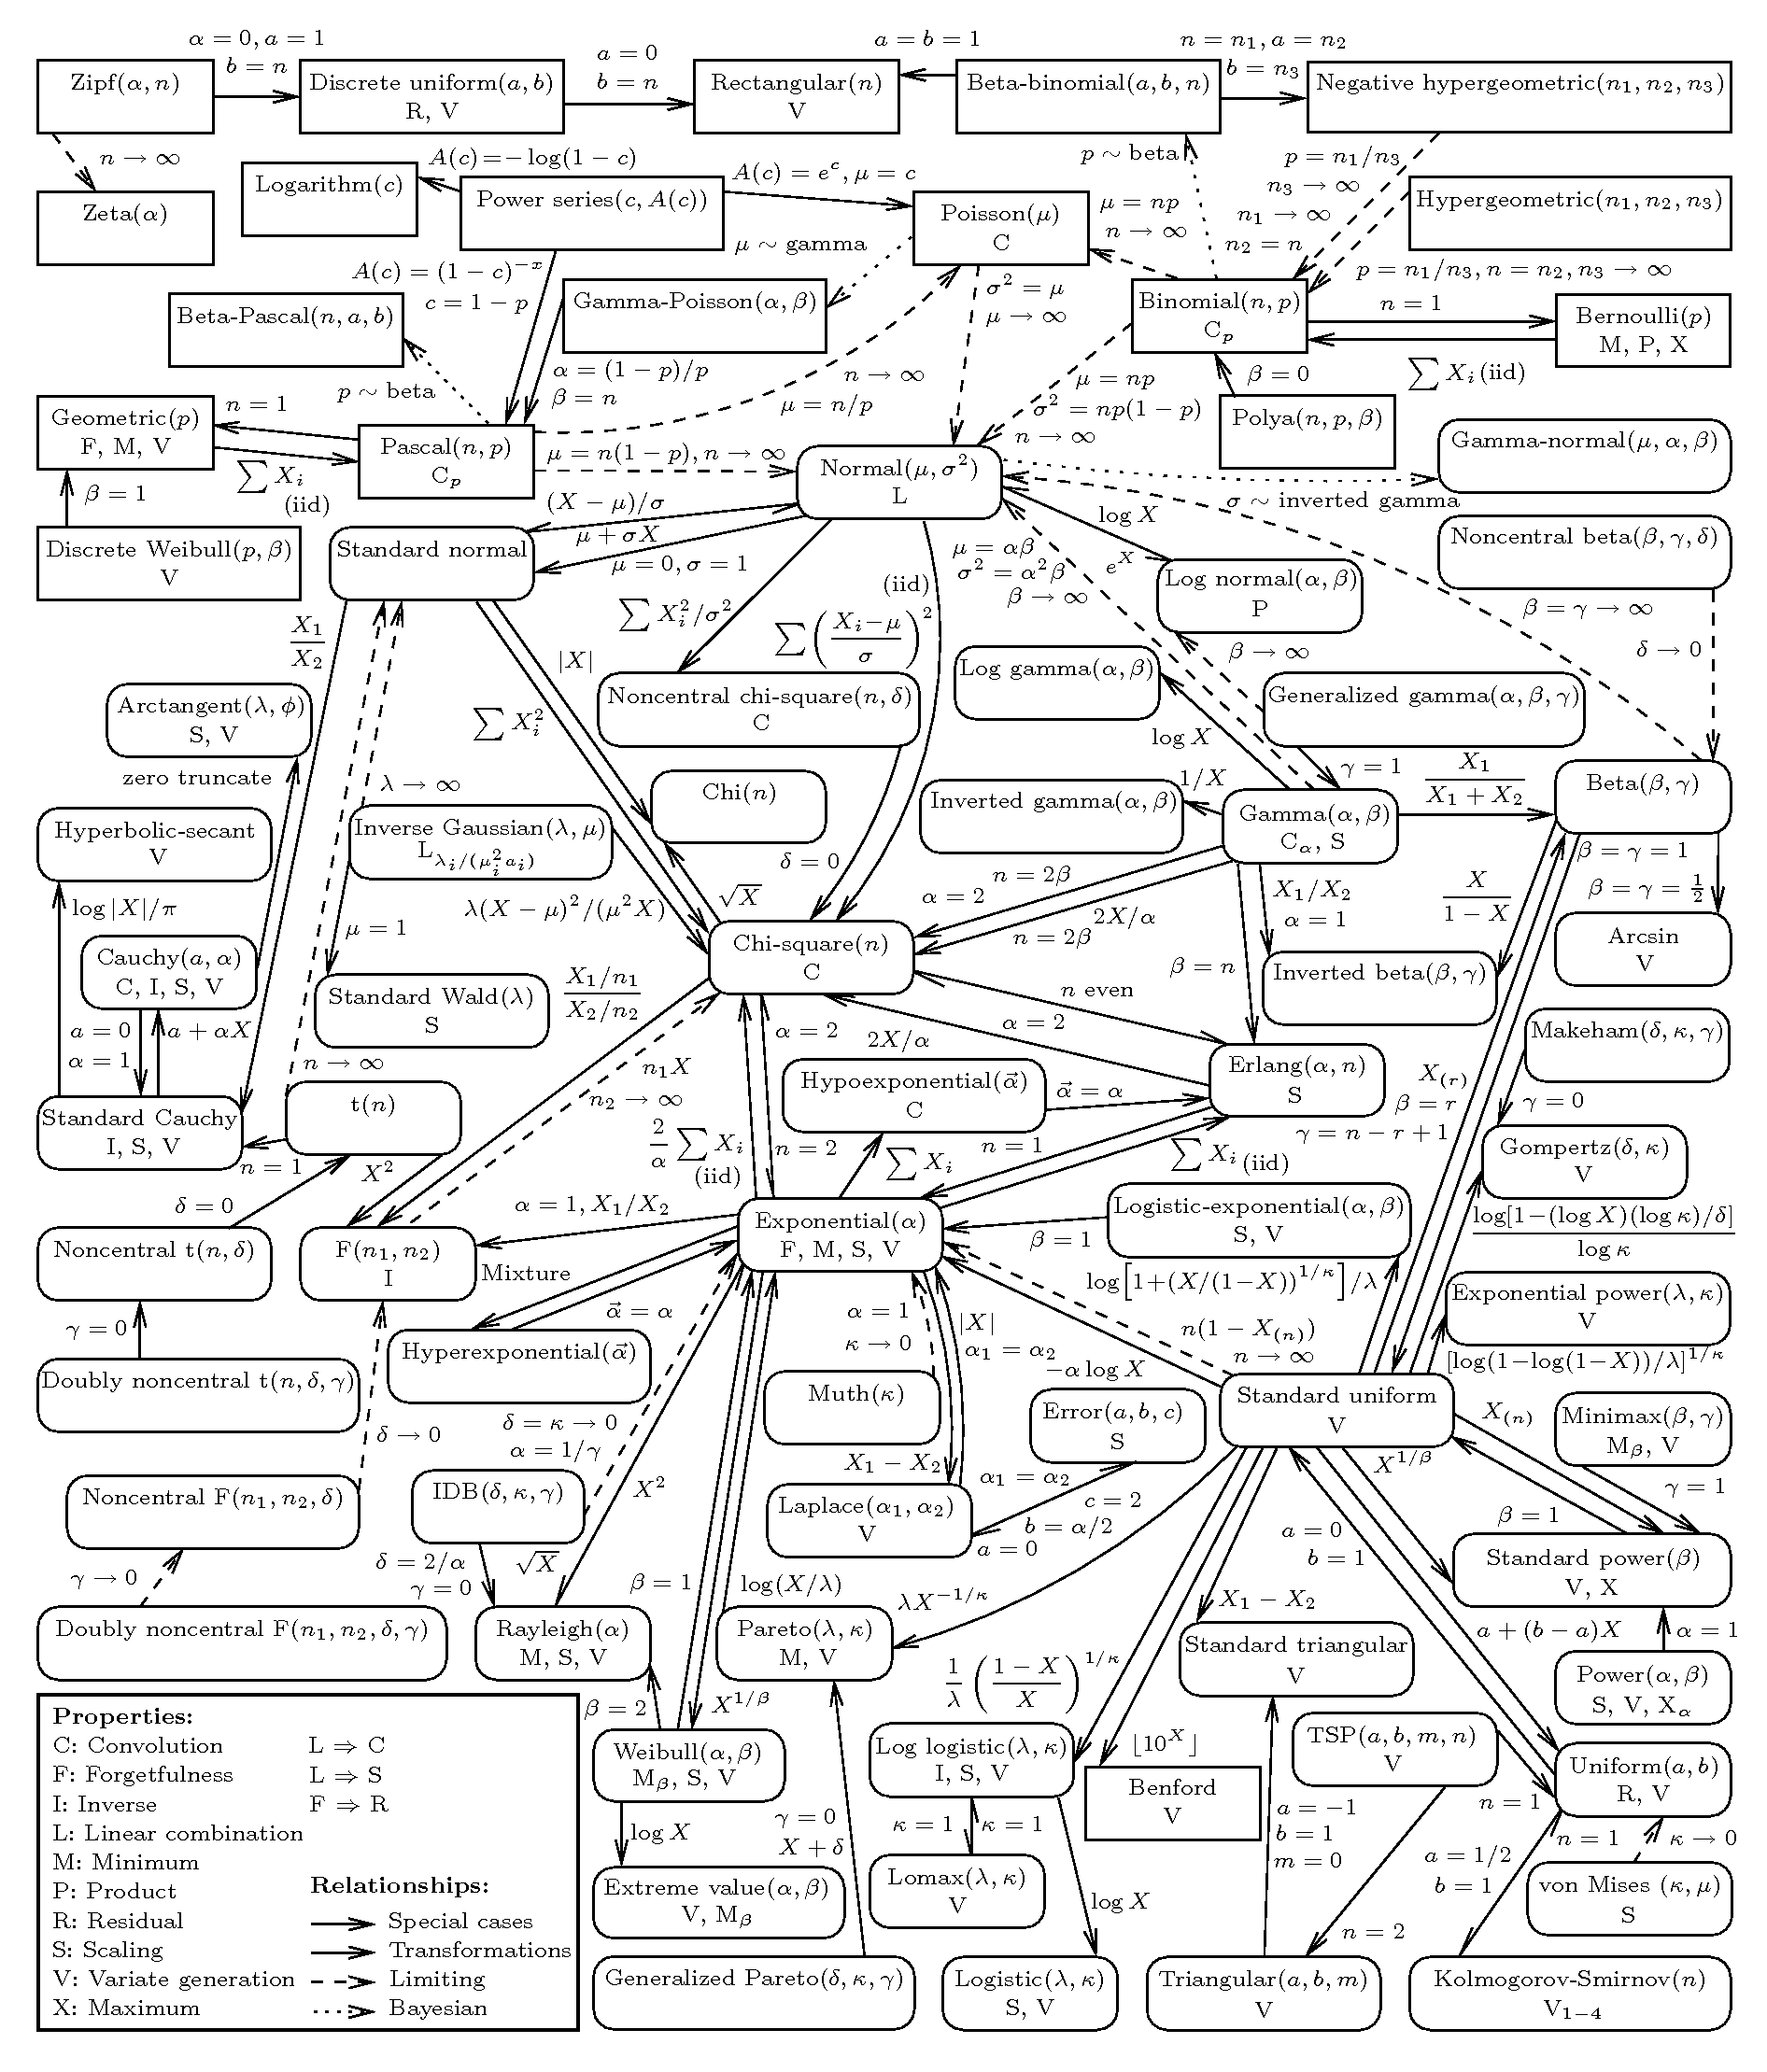
\includegraphics[width=0.5\textwidth,height=\textheight]{UnivariateDistribution.png}

\hypertarget{references}{%
\section{References}\label{references}}

\begin{tabular}{llllllllll}
\textbf{Distribution} & \textbf{CDF} & \textbf{P(X=x),f(x)} & \textbf{$\mu$} & \textbf{$EX^2$} & \textbf{Var} & \textbf{MGF} & \textbf{M'(t)} & \textbf{M''(t)} & \textbf{$M^n(t)$}\\
\hline 

$Bern(p) $ & $ $ & $p^xq^{1-x},x\in\{1,0\}$ & $p$ & $p$ & $pq$ & $pe^t+q$ \\
\hline

$Bino(n,p)$ & $I_{1-p}(n-x,x+1)$ & $ \binom{n}{x}p^x q^{n-x}; x \in \{0,1..n\}$ & $np$ & $\mu(\mu+q)$ & $\mu q$ & $(pe^t+q)^n$ \\
\hline

$Geom(p)$ & $1-q^x    $ & $pq^{x-1},x\in 1,2,..$ & $\frac1p  $ & $\frac{p+2q}{p^2} $ & $\frac{q}{p^2}$ & $\frac{pe^t}{1-qe^t},t<-\ln{q}$ \\
           & $1-q^{x+1}$ & $pq^x,x\in 0,1,..    $ & $\frac{q}p$ & $\frac{q^2+q}{p^2}$ & $\frac{q}{p^2}$ & $\frac{p}{1-qe^t}, qe^t<1     $ & $\frac{pqe^t}{(1-qe^t)^2}$ & $\frac{2pqe^t}{(1-qe^t)^3}-M'(t)$ \\
\hline

$NBino(r,p)$ & $ $ & $\binom{x-1}{r-1}p^rq^{x-r},x\in r,r+1..$ & $\frac{r}p $ & $ $ & $\frac{rq}{p^2}$ & $(\frac{pe^t}{1-qe^t})^r$\\
             & $ $ & $\binom{x+r-1}{r-1}p^rq^x, x \in 0,1..  $ & $\frac{rq}p$ & $ $ & $\frac{rq}{p^2}$ & $(\frac{p}{1-qe^t})^r, qe^t<1$\\
\hline

$HGeom(N,m,k)$ & $ $ & $\frac{\binom{m}{x}\binom{N-m}{k-x}}{\binom{N}{k}}$ & $\frac{km}{N}     $ & $ $ & $\mu\frac{(N-m)(N-k)}{N(N-1)}$ \\
$HGeom(w,b,k)$ & $ $ & $\frac{\binom{w}{x}\binom{b}{k-x}}{\binom{w+b}{k}}$ & $\frac{kw}{w+b}$ & $ $ & $\mu\frac{b(w+b-k)}{(w+b)(w+b-1)}$   \\
\hline

$Pois(\mu)$ & $e^{-\mu}\sum_{i=0}^x\frac{\mu^i}{i!}$ & $\frac{\mu^x}{x!}e^{-\mu},x \in 0,1..$ & $\mu$ & $\mu^2+\mu$ & $\mu$ & $e^{\mu(e^t-1)}$ & $\mu e^tM(t)$ & $\mu e^t(1+\mu e^t)M(t)$ \\
\hline

$Unif(n)  $ & $               $ & $ \frac{1}n,x \in 1,2..n   $ & $\frac{n+1}2  $ & $\frac{(n+1)(2n+1)}{6}$ & $\frac{(n^2-1)}{12}$ &  $\frac{\sum_{i=1}^n{e^{ti}}}n$\\
\hline
\hline

$Unif(a,b)$ & $\frac{x-a}{b-a}$ & $ \frac{1}{b-a},x \in(a,b) $ & $\frac{a+b}{2}$ & $ $& $\frac{(b-a)^2}{12}$ &  $\frac{e^{tb}-e^{ta}}{t(b-a)}$\\
\hline

$Norm(\mu,\sigma^2)$ & $ $ & $\frac{1}{\sigma\sqrt{2\pi}} e^{-\frac{(x-\mu)^2}{2\sigma^2}}$ & $\mu$ & $\mu^2+\sigma^2$ & $\sigma^2$ & $e^{\mu t +\frac{\sigma^2t^2}2}$ & $(\mu+\sigma^2t)M(t)$ & $[(\mu+\sigma^2t)^2+\sigma^2]M(t) $\\
\hline

$SNorm(0, 1)        $ & $ $ & $\frac{1}{\sqrt{2\pi}}e^{-\frac{x^2}2}$ & $0$ & $1$ & $1$ & $e^{\frac{t^2}2}$ \\
\hline

$LNorm(\mu,\sigma^2)$ & $ $ & $\frac{1}{x\sigma \sqrt{2\pi}}e^{\frac{-(\ln x-\mu)^2}{2\sigma^2}}$ & $e^{\mu+\frac{\sigma^2}2}$ & $e^{2\mu+2\sigma^2}$ & $\theta^2(e^{\sigma^2}-1)$ & $\times$\\
\hline

$Cauchy(\theta,\sigma^2)$ & $ $ & $\frac{1}{\pi\sigma}\frac1{1+(\frac{x-\theta}{\sigma})^2}$ & $\times$ & $\times$ & $\times$ & $ $ \\
\hline

$DExpo(\mu,\sigma^2)$ & $ $ & $\frac{1}{2\pi\sigma} e^{-|\frac{x-\mu}{\sigma}|}$ & $\mu$ & $\mu^2+2\sigma^2$ & $2\sigma^2$ & $\frac{e^{\mu t}}{1-\sigma^2t^2}$ \\
\hline

$Expo(\lambda)$ & $1-e^{-\lambda x}$ & $\lambda e^{-\lambda x},x \in (0,\infty)$ & $\frac{1}{\lambda}$ & $ $ & $\frac{1}{\lambda^2}$ & $\frac{\lambda}{\lambda - t}, t < \lambda$\\
$Expo(\beta)  $ & $                $ & $\frac1{\beta} e^{-\frac{x}\beta}$ & $\beta$ & $ $ & $\beta^2$ & $\frac{1}{1-\beta t}$ & $\beta(1-\beta t)^{-2}$ & $2\beta^2(1-\beta t)^{-3}$\\
\hline

$Gammma(a, \lambda)$ & $ $ & $\frac{\lambda^a}{\Gamma(a)}x^{a-1}e^{-\lambda x},x \in (0,\infty)$ & $\frac{a}{\lambda}$  & $\frac{a}{\lambda^2}$ & $\left(\frac{\lambda}{\lambda - t}\right)^a, t < \lambda$\\
$Gammma(\alpha,\beta)$ & $ $ & $\frac{1}{\Gamma(a)\beta^{\alpha}}x^{a-1}e^{-x/\beta}$ & $\alpha\beta$  & $\alpha\beta^2$ & $\left(\frac{1}{1-\beta t}\right)^a, t <\frac1\beta$\\
\hline

$Beta(a, b)$ & $ $ & $\frac{\Gamma(a+b)}{\Gamma(a)\Gamma(b)}x^{a-1}(1-x)^{b-1} $ & $\frac{a}{a+b}$ & $ $  & $\frac{\mu(1-\mu)}{(a+b+1)}$ & $ $ & $ $ & $ $ & $\frac{\Gamma(\alpha+n)\Gamma(\alpha+\beta)}{\Gamma(\alpha+\beta+n)\Gamma(\alpha)}$  \\
$B(\alpha,\beta)=$ & $ $ & $\frac{\Gamma(\alpha)\Gamma(\beta)}{\Gamma(\alpha+\beta)},x\in(0,1)$ & $ $  & $\frac{a(a+1)}{(a+b)(a+b+1)}$ & $\frac{ab}{(a+b)^2(a+b+1)}$ \\
\hline

$\chi_p^2$ & $ $ & $\frac{x^{\frac{p}2-1}}{\Gamma \frac{p}2 2^{\frac{p}2}}e^{-\frac{x}2}$ & $p$ & $2p+p^2$ & $2p$ & $(1-2t)^{-p/2}, t<\frac12$\\
\hline

$t_p$ & $ $ & $\frac{\Gamma(\frac{p+1}2)}{\Gamma(\frac{p}2)\sqrt{p\pi}}\left (1+\frac{x^2}{p}\right)^{-\frac{p+1}2}$ & $0,p>1$ & $ $ & $\frac{p}{p-2},p>2$ & $\times$\\
\hline

$F$ & $x>0$ & $\frac{\Gamma(\frac{p+q}2)}{\Gamma(\frac{p}2)\Gamma (\frac{q}2)}(\frac{p}q)^{\frac{p}2}\frac{x^{\frac{p}2-1}}{(1+\frac{p}qx)^{\frac{p+q}2}}$ & $\frac{q}{q-2}$ & $q>2$ & $2(\frac{q}{q-2})^2\frac{p+q-2}{p(q-4)}$ & $q>4$\\
\hline

Arcsine & $\frac{1}{\pi \arcsin\sqrt x}$ & $\frac{1}{\pi\sqrt{x(1-x)}},x\in[0,1]$ & $\frac{1}2$ & $ $ & $\frac{1}8$ & & & & $Beta(\frac{1}2,\frac{1}2)$\\
\hline

Dirichlet & $B(a)=\frac{\Pi_{i=1}^k\Gamma(a_i)}{\Gamma(\sum_{i=1}^ka_i)}$ & $\frac1{B(a)}\Pi_{i=1}^kx_i^{a_i-1},x\in(0,1)$ & $\frac{a_i}{\sum_ka_k}$ & $\sum_{i=1}^kx_i=1$ & $\frac{a_i(a_0-a_i)}{a_0^2(a_0+1)}$ & $Cov(X_i,X_j)=$ & $\frac{-a_ia_j}{a_0^2(a_0+1)}$ & $a_0=\sum_{i=1}^ka_i$ & \\
\hline

\end{tabular}


\end{document}
